\documentclass[twoside]{book}

% Packages required by doxygen
\usepackage{fixltx2e}
\usepackage{calc}
\usepackage{doxygen}
\usepackage{graphicx}
\usepackage[utf8]{inputenc}
\usepackage{makeidx}
\usepackage{multicol}
\usepackage{multirow}
\PassOptionsToPackage{warn}{textcomp}
\usepackage{textcomp}
\usepackage[nointegrals]{wasysym}
\usepackage[table]{xcolor}

% Font selection
\usepackage[T1]{fontenc}
\usepackage[scaled=.90]{helvet}
\usepackage{courier}
\usepackage{amssymb}
\usepackage{sectsty}
\renewcommand{\familydefault}{\sfdefault}
\allsectionsfont{%
  \fontseries{bc}\selectfont%
  \color{darkgray}%
}
\renewcommand{\DoxyLabelFont}{%
  \fontseries{bc}\selectfont%
  \color{darkgray}%
}
\newcommand{\+}{\discretionary{\mbox{\scriptsize$\hookleftarrow$}}{}{}}

% Page & text layout
\usepackage{geometry}
\geometry{%
  a4paper,%
  top=2.5cm,%
  bottom=2.5cm,%
  left=2.5cm,%
  right=2.5cm%
}
\tolerance=750
\hfuzz=15pt
\hbadness=750
\setlength{\emergencystretch}{15pt}
\setlength{\parindent}{0cm}
\setlength{\parskip}{0.2cm}
\makeatletter
\renewcommand{\paragraph}{%
  \@startsection{paragraph}{4}{0ex}{-1.0ex}{1.0ex}{%
    \normalfont\normalsize\bfseries\SS@parafont%
  }%
}
\renewcommand{\subparagraph}{%
  \@startsection{subparagraph}{5}{0ex}{-1.0ex}{1.0ex}{%
    \normalfont\normalsize\bfseries\SS@subparafont%
  }%
}
\makeatother

% Headers & footers
\usepackage{fancyhdr}
\pagestyle{fancyplain}
\fancyhead[LE]{\fancyplain{}{\bfseries\thepage}}
\fancyhead[CE]{\fancyplain{}{}}
\fancyhead[RE]{\fancyplain{}{\bfseries\leftmark}}
\fancyhead[LO]{\fancyplain{}{\bfseries\rightmark}}
\fancyhead[CO]{\fancyplain{}{}}
\fancyhead[RO]{\fancyplain{}{\bfseries\thepage}}
\fancyfoot[LE]{\fancyplain{}{}}
\fancyfoot[CE]{\fancyplain{}{}}
\fancyfoot[RE]{\fancyplain{}{\bfseries\scriptsize Generated on Mon Nov 10 2014 15\+:08\+:11 for Fuse\+A\+P\+I (i\+O\+S) by Doxygen }}
\fancyfoot[LO]{\fancyplain{}{\bfseries\scriptsize Generated on Mon Nov 10 2014 15\+:08\+:11 for Fuse\+A\+P\+I (i\+O\+S) by Doxygen }}
\fancyfoot[CO]{\fancyplain{}{}}
\fancyfoot[RO]{\fancyplain{}{}}
\renewcommand{\footrulewidth}{0.4pt}
\renewcommand{\chaptermark}[1]{%
  \markboth{#1}{}%
}
\renewcommand{\sectionmark}[1]{%
  \markright{\thesection\ #1}%
}

% Indices & bibliography
\usepackage{natbib}
\usepackage[titles]{tocloft}
\setcounter{tocdepth}{3}
\setcounter{secnumdepth}{5}
\makeindex

% Hyperlinks (required, but should be loaded last)
\usepackage{ifpdf}
\ifpdf
  \usepackage[pdftex,pagebackref=true]{hyperref}
\else
  \usepackage[ps2pdf,pagebackref=true]{hyperref}
\fi
\hypersetup{%
  colorlinks=true,%
  linkcolor=blue,%
  citecolor=blue,%
  unicode%
}

% Custom commands
\newcommand{\clearemptydoublepage}{%
  \newpage{\pagestyle{empty}\cleardoublepage}%
}


%===== C O N T E N T S =====

\begin{document}

% Titlepage & ToC
\hypersetup{pageanchor=false,
             bookmarks=true,
             bookmarksnumbered=true,
             pdfencoding=unicode
            }
\pagenumbering{roman}
\begin{titlepage}
\vspace*{7cm}
\begin{center}%
{\Large Fuse\+A\+P\+I (i\+O\+S) }\\
\vspace*{1cm}
{\large Generated by Doxygen 1.8.8}\\
\vspace*{0.5cm}
{\small Mon Nov 10 2014 15:08:11}\\
\end{center}
\end{titlepage}
\clearemptydoublepage
\tableofcontents
\clearemptydoublepage
\pagenumbering{arabic}
\hypersetup{pageanchor=true}

%--- Begin generated contents ---
\chapter{Deprecated List}
\label{deprecated}
\hypertarget{deprecated}{}

\begin{DoxyRefList}
\item[\label{deprecated__deprecated000002}%
\hypertarget{deprecated__deprecated000002}{}%
Global \hyperlink{interface_fuse_s_d_k_a04c181e3ec49e81ba081a5041df412f6}{\mbox{[}Fuse\+S\+D\+K facebook\+Login\+:\mbox{]}} ]Since \hyperlink{interface_fuse_s_d_k}{Fuse\+S\+D\+K} version 1.\+23. See facebook\+Login\+:\+Name\+:with\+Access\+Token\+: for more information on new method.  
\item[\label{deprecated__deprecated000001}%
\hypertarget{deprecated__deprecated000001}{}%
Global \hyperlink{interface_fuse_s_d_k_aa37c46cc4e49f09fd9b2b40a548b61fc}{\mbox{[}Fuse\+S\+D\+K respond\+To\+Application\+Launch\+Options\+:Application\+:\mbox{]}} ]This method is deprecated and will be removed 
\end{DoxyRefList}
\chapter{Hierarchical Index}
\section{Class Hierarchy}
This inheritance list is sorted roughly, but not completely, alphabetically\+:\begin{DoxyCompactList}
\item $<$N\+S\+Object$>$\begin{DoxyCompactList}
\item \contentsline{section}{$<$Fuse\+Ad\+Delegate$>$}{\pageref{protocol_fuse_ad_delegate-p}}{}
\item \contentsline{section}{Fuse\+A\+P\+I}{\pageref{interface_fuse_a_p_i}}{}
\item \contentsline{section}{$<$Fuse\+Delegate$>$}{\pageref{protocol_fuse_delegate-p}}{}
\item \contentsline{section}{$<$Fuse\+Game\+Data\+Delegate$>$}{\pageref{protocol_fuse_game_data_delegate-p}}{}
\item \contentsline{section}{$<$Fuse\+Overlay\+Delegate$>$}{\pageref{protocol_fuse_overlay_delegate-p}}{}
\end{DoxyCompactList}
\end{DoxyCompactList}

\chapter{Data Structure Index}
\section{Data Structures}
Here are the data structures with brief descriptions\+:\begin{DoxyCompactList}
\item\contentsline{section}{\hyperlink{protocol_fuse_delegate-p}{$<$\+Fuse\+Delegate$>$} \\*This is the Fuse S\+D\+K delegate }{\pageref{protocol_fuse_delegate-p}}{}
\item\contentsline{section}{\hyperlink{interface_fuse_i_a_p_offer_object}{Fuse\+I\+A\+P\+Offer\+Object} \\*Object Returned to the S\+D\+K when a I\+A\+P offer was Accepted, }{\pageref{interface_fuse_i_a_p_offer_object}}{}
\item\contentsline{section}{\hyperlink{interface_fuse_rewarded_object}{Fuse\+Rewarded\+Object} \\*Object Returned to the S\+D\+K when a rewarded Ad was completed, }{\pageref{interface_fuse_rewarded_object}}{}
\item\contentsline{section}{\hyperlink{interface_fuse_s_d_k}{Fuse\+S\+D\+K} \\*This is the main Fuse S\+D\+K static class }{\pageref{interface_fuse_s_d_k}}{}
\item\contentsline{section}{\hyperlink{interface_fuse_virtual_goods_offer_object}{Fuse\+Virtual\+Goods\+Offer\+Object} \\*Object Returned to the S\+D\+K when a Virtual Goods offer was Accepted, }{\pageref{interface_fuse_virtual_goods_offer_object}}{}
\end{DoxyCompactList}

\chapter{Data Structure Documentation}
\hypertarget{protocol_fuse_ad_delegate-p}{}\section{$<$Fuse\+Ad\+Delegate$>$ Protocol Reference}
\label{protocol_fuse_ad_delegate-p}\index{$<$\+Fuse\+Ad\+Delegate$>$@{$<$\+Fuse\+Ad\+Delegate$>$}}


This is Fuse A\+P\+I ad delegate.  




{\ttfamily \#import $<$Fuse\+A\+P\+I.\+h$>$}

Inheritance diagram for $<$Fuse\+Ad\+Delegate$>$\+:\begin{figure}[H]
\begin{center}
\leavevmode
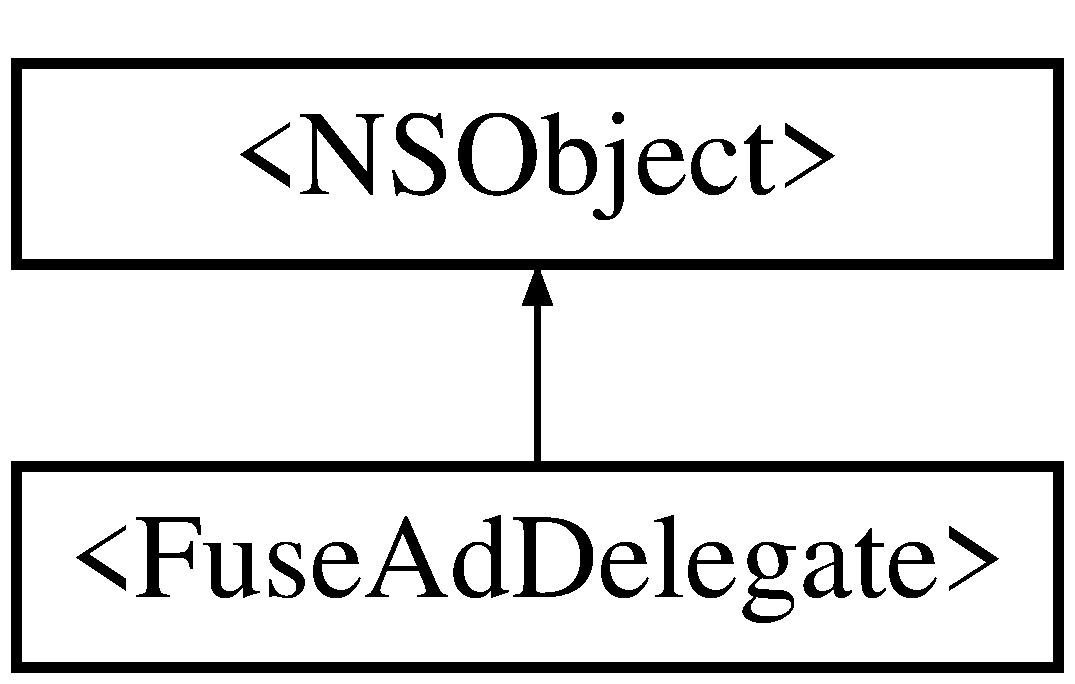
\includegraphics[height=2.000000cm]{protocol_fuse_ad_delegate-p}
\end{center}
\end{figure}
\subsection*{Instance Methods}
\begin{DoxyCompactItemize}
\item 
(void) -\/ \hyperlink{protocol_fuse_ad_delegate-p_aafc293cd46be3bd70eeb60971b961a51}{ad\+Will\+Close}
\begin{DoxyCompactList}\small\item\em This method indicates when a full-\/screen (interstitial) ad is closing. \end{DoxyCompactList}\end{DoxyCompactItemize}


\subsection{Detailed Description}
This is Fuse A\+P\+I ad delegate. 

Handles all notifications involved with showing an ad and responding to an ad closing. 

\subsection{Method Documentation}
\hypertarget{protocol_fuse_ad_delegate-p_aafc293cd46be3bd70eeb60971b961a51}{}\index{Fuse\+Ad\+Delegate-\/p@{Fuse\+Ad\+Delegate-\/p}!ad\+Will\+Close@{ad\+Will\+Close}}
\index{ad\+Will\+Close@{ad\+Will\+Close}!Fuse\+Ad\+Delegate-\/p@{Fuse\+Ad\+Delegate-\/p}}
\subsubsection[{ad\+Will\+Close}]{\setlength{\rightskip}{0pt plus 5cm}-\/ (void) ad\+Will\+Close 
\begin{DoxyParamCaption}
{}
\end{DoxyParamCaption}
\hspace{0.3cm}{\ttfamily [required]}}\label{protocol_fuse_ad_delegate-p_aafc293cd46be3bd70eeb60971b961a51}


This method indicates when a full-\/screen (interstitial) ad is closing. 

When an ad is being dismissed by the user and control is to be returned to the application, this method will be called. Once called, the application can continue execution of the user flow or application. \begin{DoxySeeAlso}{See also}
\hyperlink{interface_fuse_a_p_i_ada82ae54afd63865982e516d4a71a8b5}{+ show\+Ad\+With\+Delegate\+: (\+Fuse\+A\+P\+I)} for more information on displaying an ad with a $<$\hyperlink{protocol_fuse_ad_delegate-p}{Fuse\+Ad\+Delegate}$>$ 
\end{DoxySeeAlso}
\begin{DoxySince}{Since}
\hyperlink{interface_fuse_a_p_i}{Fuse\+A\+P\+I} version 1.\+12 
\end{DoxySince}


The documentation for this protocol was generated from the following file\+:\begin{DoxyCompactItemize}
\item 
/\+Users/buildmachine/buildmonkey/\+Fuse\+S\+D\+Ki\+O\+S-\/master/\+Code/\+Classes/\+Fuse\+A\+P\+I/Fuse\+A\+P\+I.\+h\end{DoxyCompactItemize}

\hypertarget{interface_fuse_a_p_i}{}\section{Fuse\+A\+P\+I Class Reference}
\label{interface_fuse_a_p_i}\index{Fuse\+A\+P\+I@{Fuse\+A\+P\+I}}


This is the main Fuse A\+P\+I static class.  




{\ttfamily \#import $<$Fuse\+A\+P\+I.\+h$>$}

Inheritance diagram for Fuse\+A\+P\+I\+:\begin{figure}[H]
\begin{center}
\leavevmode
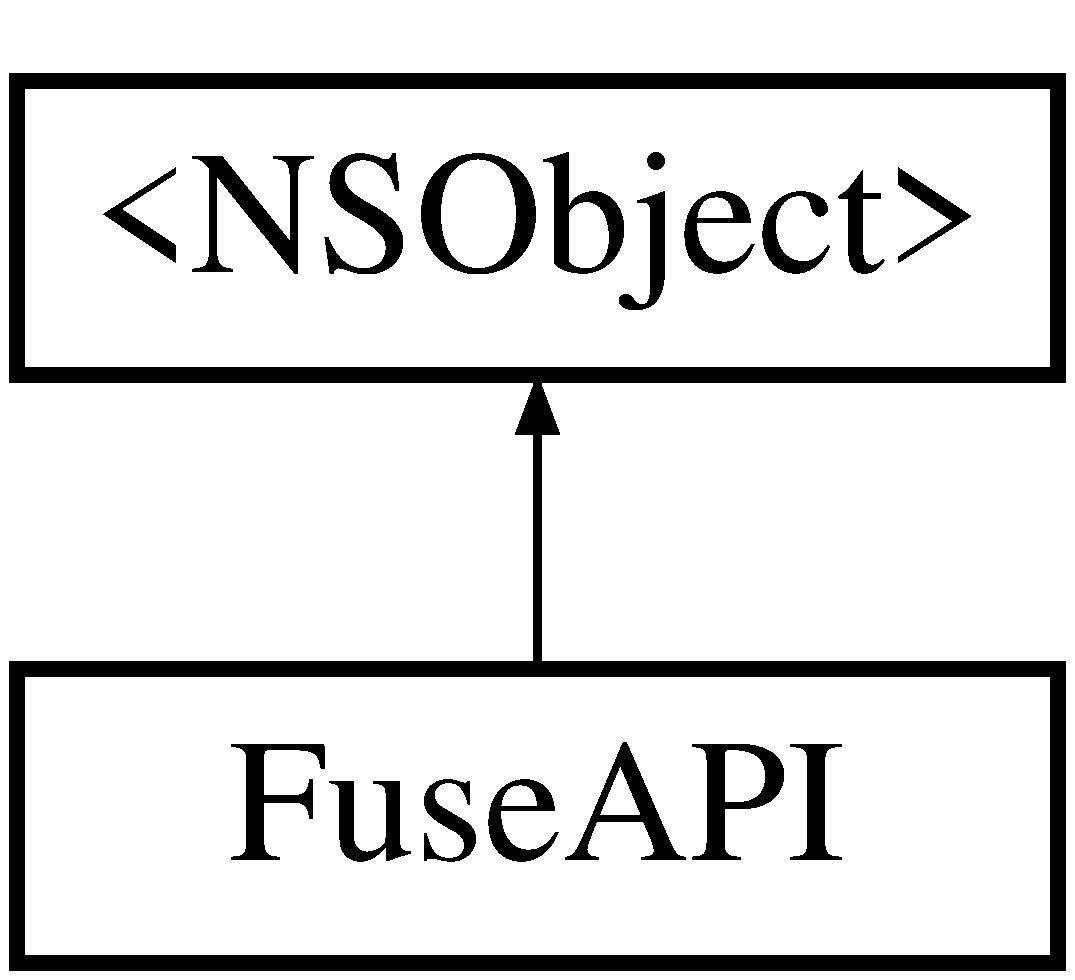
\includegraphics[height=2.000000cm]{interface_fuse_a_p_i}
\end{center}
\end{figure}
\subsection*{Class Methods}
\begin{DoxyCompactItemize}
\item 
(void) + \hyperlink{interface_fuse_a_p_i_ab8c3327287bfed0a8a9c74e6664d7717}{start\+Session\+:}
\begin{DoxyCompactList}\small\item\em This method is used to initiate all communication with the Fuse system. \end{DoxyCompactList}\item 
(void) + \hyperlink{interface_fuse_a_p_i_aab1649c81002a336ca872da6fef36b8d}{start\+Session\+:\+Delegate\+:}
\begin{DoxyCompactList}\small\item\em This method is used to initiate all communication with the Fuse system (and register a $<$\hyperlink{protocol_fuse_delegate-p}{Fuse\+Delegate}$>$) \end{DoxyCompactList}\item 
(void) + \hyperlink{interface_fuse_a_p_i_aa08196a04aa0f91f8967e2f0cd9b5f6e}{start\+Session\+:\+Delegate\+:\+Auto\+Register\+For\+Push\+:}
\begin{DoxyCompactList}\small\item\em This method is used to initiate all communication with the Fuse system (and register a $<$\hyperlink{protocol_fuse_delegate-p}{Fuse\+Delegate}$>$) \end{DoxyCompactList}\item 
(void) + \hyperlink{interface_fuse_a_p_i_a4400b7bb4b8e108c38405c47eba69b5c}{set\+Platform\+:}
\begin{DoxyCompactList}\small\item\em This method is used to describe the platform the A\+P\+I is running on. \end{DoxyCompactList}\item 
(void) + \hyperlink{interface_fuse_a_p_i_aea1b9766935aafaeb49889dc6f7cca93}{register\+For\+Push\+Token}
\begin{DoxyCompactList}\small\item\em This method is used to manually register for a push notification device token. \end{DoxyCompactList}\item 
(void) + \hyperlink{interface_fuse_a_p_i_a774f0872e0eb00528391cdc376876446}{register\+For\+Push\+Token\+:}
\begin{DoxyCompactList}\small\item\em This method is used to manually register for a push notification device token. \end{DoxyCompactList}\item 
(void) + \hyperlink{interface_fuse_a_p_i_a94479850c3b0c60887b96bb9cfa714e6}{applicationdid\+Register\+For\+Remote\+Notifications\+With\+Device\+Token\+:}
\begin{DoxyCompactList}\small\item\em This method is used to pass the registered Apple push token to the Fuse servers for future push notification messaging. \end{DoxyCompactList}\item 
(void) + \hyperlink{interface_fuse_a_p_i_ac3d0b5c1336b7a2883a6693fd4696ea0}{applicationdid\+Fail\+To\+Register\+For\+Remote\+Notifications\+With\+Error\+:}
\begin{DoxyCompactList}\small\item\em This method is used to capture when the registration of a device token has failed. \end{DoxyCompactList}\item 
(void) + \hyperlink{interface_fuse_a_p_i_a527313014384e35bf0537595295e1224}{applicationdid\+Receive\+Remote\+Notification\+:\+Application\+:}
\begin{DoxyCompactList}\small\item\em This method is used to capture when a user either receives an Apple push notification when the application is running or chooses to re-\/enter the application because of a click on an on-\/of-\/application notification . \end{DoxyCompactList}\item 
(void) + \hyperlink{interface_fuse_a_p_i_aa37c46cc4e49f09fd9b2b40a548b61fc}{respond\+To\+Application\+Launch\+Options\+:\+Application\+:}
\begin{DoxyCompactList}\small\item\em This method is optional and can collect launch options. \end{DoxyCompactList}\item 
(void) + \hyperlink{interface_fuse_a_p_i_a36deac5ef469d2f0e0b2f17fa2398a65}{register\+Event\+:}
\begin{DoxyCompactList}\small\item\em This method is used to register an named event in the Fuse system. \end{DoxyCompactList}\item 
(int) + \hyperlink{interface_fuse_a_p_i_ad5bc4fce3b1c795ca55beab32c9b600d}{register\+Event\+:with\+Dict\+:}
\begin{DoxyCompactList}\small\item\em This method is used to register an named event in the Fuse system. \end{DoxyCompactList}\item 
(int) + \hyperlink{interface_fuse_a_p_i_a837bfdf6d8a8dfa5f1693f3309734bf9}{register\+Event\+:\+Parameter\+Name\+:\+Parameter\+Value\+:\+Variables\+:}
\begin{DoxyCompactList}\small\item\em This method will send a named event (with values) to the Fuse system for tracking. \end{DoxyCompactList}\item 
(int) + \hyperlink{interface_fuse_a_p_i_a1ffe87df7aec0f432ef815a84e4750d8}{register\+Event\+:\+Parameter\+Name\+:\+Parameter\+Value\+:\+Variable\+Name\+:\+Variable\+Value\+:}
\begin{DoxyCompactList}\small\item\em This method will send a named event (with values) to the Fuse system for tracking. \end{DoxyCompactList}\item 
(void) + \hyperlink{interface_fuse_a_p_i_a9afd8c386a2b6664641da19fa64072c9}{register\+Crash\+:}
\begin{DoxyCompactList}\small\item\em This method is used to catch crashes within an app. \end{DoxyCompactList}\item 
(void) + \hyperlink{interface_fuse_a_p_i_ab1029e5beb592f22c1ba0deea9e7bd1c}{register\+In\+App\+Purchase\+List\+:}
\begin{DoxyCompactList}\small\item\em This method is used to register the price and currency that a user is using to make an in-\/app purchase. \end{DoxyCompactList}\item 
(void) + \hyperlink{interface_fuse_a_p_i_a2dd50722daab117889c396ff58fe7c27}{register\+In\+App\+Purchase\+:}
\begin{DoxyCompactList}\small\item\em This method records in-\/app purchases in the Fuse system. \end{DoxyCompactList}\item 
(void) + \hyperlink{interface_fuse_a_p_i_a8a1846c84fa16e45488e797dca4c7aaa}{register\+In\+App\+Purchase\+:\+Tx\+State\+:\+Price\+:\+Currency\+:\+Product\+I\+D\+:}
\begin{DoxyCompactList}\small\item\em This method records in-\/app purchases in the Fuse system without using the S\+K\+Payment\+Transaction data type. \end{DoxyCompactList}\item 
(void) + \hyperlink{interface_fuse_a_p_i_a2115a4fac03204fd73699ab9ea3314f5}{register\+In\+App\+Purchase\+:\+Tx\+State\+:\+Price\+:\+Currency\+:\+Product\+I\+D\+:\+Transaction\+I\+D\+:}
\begin{DoxyCompactList}\small\item\em This method records in-\/app purchases in the Fuse system without using the S\+K\+Payment\+Transaction data type. \end{DoxyCompactList}\item 
(void) + \hyperlink{interface_fuse_a_p_i_ada82ae54afd63865982e516d4a71a8b5}{show\+Ad\+With\+Delegate\+:}
\begin{DoxyCompactList}\small\item\em This method is used to display a Fuse interstitial ad within the application. \end{DoxyCompactList}\item 
(void) + \hyperlink{interface_fuse_a_p_i_a77f8d91d1491f0ad94bc1f0ca3fb7993}{show\+Ad\+With\+Delegate\+:ad\+Zone\+:}
\begin{DoxyCompactList}\small\item\em This method displays a Fuse interstitial ad for a given ad zone. Different ad zones can be configured via the Fuse Dashboard. \end{DoxyCompactList}\item 
(void) + \hyperlink{interface_fuse_a_p_i_a5813b52f07d4818a4e97ceb9829a0786}{check\+Ad\+Available}
\begin{DoxyCompactList}\small\item\em This method indicates whether an ad is available to be shown to the user. \end{DoxyCompactList}\item 
(void) + \hyperlink{interface_fuse_a_p_i_a3c9bb1034fabe54bb67b21503cf74311}{check\+Ad\+Available\+With\+Delegate\+:}
\begin{DoxyCompactList}\small\item\em This method indicates whether an ad is available to be shown to the user. \end{DoxyCompactList}\item 
(void) + \hyperlink{interface_fuse_a_p_i_a12f119c6dd8ea610f5f2a376a0c6f7a5}{check\+Ad\+Available\+With\+Delegate\+:with\+Ad\+Zone\+:}
\begin{DoxyCompactList}\small\item\em This method indicates whether an ad is available to be shown to the user for the specified ad zone. \end{DoxyCompactList}\item 
(void) + \hyperlink{interface_fuse_a_p_i_a0f4ef6867a87c0a565849c96dd0f31fa}{pre\+Load\+Ad\+For\+Zone\+:}
\begin{DoxyCompactList}\small\item\em This method preloads an ad for a specified ad zone. \end{DoxyCompactList}\item 
(void) + \hyperlink{interface_fuse_a_p_i_a279e4cb8e95a3e78197761156a7de50d}{display\+Notifications}
\begin{DoxyCompactList}\small\item\em This method is used to display in-\/game Fuse notifications. \end{DoxyCompactList}\item 
\hypertarget{interface_fuse_a_p_i_a23c30bc15f208daf639ece250b8a5935}{}(B\+O\+O\+L) + \hyperlink{interface_fuse_a_p_i_a23c30bc15f208daf639ece250b8a5935}{is\+Notification\+Available}\label{interface_fuse_a_p_i_a23c30bc15f208daf639ece250b8a5935}

\begin{DoxyCompactList}\small\item\em This method returns whether a Fuse notification is available to be viewed. \end{DoxyCompactList}\item 
(void) + \hyperlink{interface_fuse_a_p_i_aced6aa0cc51278b431c664c3f5f9fc30}{display\+More\+Games\+:}
\begin{DoxyCompactList}\small\item\em This method is use to display the \char`\"{}\+More Games\char`\"{} section. \end{DoxyCompactList}\item 
(void) + \hyperlink{interface_fuse_a_p_i_a2b0c7be7abc4ec4ae6912f295d21e64c}{register\+Gender\+:}
\begin{DoxyCompactList}\small\item\em This method registers a gender for the user. \end{DoxyCompactList}\item 
(void) + \hyperlink{interface_fuse_a_p_i_a33903ca8d52be440186c4bbf1cbe510c}{register\+Age\+:}
\begin{DoxyCompactList}\small\item\em This method registers an age for the user. \end{DoxyCompactList}\item 
(void) + \hyperlink{interface_fuse_a_p_i_a5dcbaec8b00d90c4970e1b752e5dc719}{register\+Birthday\+:\+Month\+:\+Day\+:}
\begin{DoxyCompactList}\small\item\em This method registers a user's birthday. \end{DoxyCompactList}\item 
(N\+S\+String $\ast$) + \hyperlink{interface_fuse_a_p_i_ab483c2a3f4439aad8e19200cf24ff731}{get\+Fuse\+I\+D}
\begin{DoxyCompactList}\small\item\em This method returns the public 'Fuse I\+D'. \end{DoxyCompactList}\item 
(void) + \hyperlink{interface_fuse_a_p_i_a02a3bc5562d4f6e50bac5339f4ac4046}{game\+Center\+Login\+:}
\begin{DoxyCompactList}\small\item\em Game Center account registration. \end{DoxyCompactList}\item 
(void) + \hyperlink{interface_fuse_a_p_i_a7003a2102cba9c87fa127e39c95a5d1d}{facebook\+Login\+:\+Name\+:with\+Access\+Token\+:}
\begin{DoxyCompactList}\small\item\em Facebook account registration. \end{DoxyCompactList}\item 
(void) + \hyperlink{interface_fuse_a_p_i_a04c181e3ec49e81ba081a5041df412f6}{facebook\+Login\+:}
\begin{DoxyCompactList}\small\item\em Facebook account registration. \end{DoxyCompactList}\item 
(void) + \hyperlink{interface_fuse_a_p_i_a38487be821059910b1b939d818cd0e9f}{facebook\+Login\+:\+Name\+:\+Gender\+:with\+Access\+Token\+:}
\begin{DoxyCompactList}\small\item\em Facebook account registration. \end{DoxyCompactList}\item 
(void) + \hyperlink{interface_fuse_a_p_i_add5138c113d6e4c1201f70bf8b84eb02}{twitter\+Login\+:}
\begin{DoxyCompactList}\small\item\em Twitter account registration. \end{DoxyCompactList}\item 
(void) + \hyperlink{interface_fuse_a_p_i_a48950b5880ce336cc601a752bcda1a3a}{twitter\+Login\+:\+Alias\+:}
\begin{DoxyCompactList}\small\item\em Twitter account registration with user name. \end{DoxyCompactList}\item 
(void) + \hyperlink{interface_fuse_a_p_i_ae7db839fcdcf674aa1e456a16655e614}{open\+Feint\+Login\+:}
\begin{DoxyCompactList}\small\item\em Open\+Feint account registration. \end{DoxyCompactList}\item 
(void) + \hyperlink{interface_fuse_a_p_i_af7b69ec93b7a26b8512d730db9383511}{fuse\+Login\+:\+Alias\+:}
\begin{DoxyCompactList}\small\item\em Fuse account registration. \end{DoxyCompactList}\item 
(void) + \hyperlink{interface_fuse_a_p_i_a6b16a24e8cb2fdd04b8be9e501259135}{email\+Login\+:\+Alias\+:}
\begin{DoxyCompactList}\small\item\em Account registration using an email address. \end{DoxyCompactList}\item 
(void) + \hyperlink{interface_fuse_a_p_i_ae3a27f858739fee7ad6483a909206943}{device\+Login\+:}
\begin{DoxyCompactList}\small\item\em Account registration using the unique device identifier. \end{DoxyCompactList}\item 
(void) + \hyperlink{interface_fuse_a_p_i_a826545aa45a550cbc10cc98137ee5898}{google\+Play\+Login\+:\+Access\+Token\+:}
\begin{DoxyCompactList}\small\item\em Account registration using the google play login identifier. \end{DoxyCompactList}\item 
(N\+S\+String $\ast$) + \hyperlink{interface_fuse_a_p_i_a49b43f13a0efee7d2af60197d0ae341c}{get\+Original\+Account\+I\+D}
\begin{DoxyCompactList}\small\item\em Get the original account I\+D used to log in to the Fuse system that corresponds to the Fuse I\+D. \end{DoxyCompactList}\item 
(int) + \hyperlink{interface_fuse_a_p_i_a0571f2d960109dc9bff59c6575bf2534}{get\+Original\+Account\+Type}
\begin{DoxyCompactList}\small\item\em Get the original account type used to log in to the Fuse system that corresponds to the Fuse I\+D. \end{DoxyCompactList}\item 
(N\+S\+String $\ast$) + \hyperlink{interface_fuse_a_p_i_ab49bb189bd1ebaf871f24a7c4e4b5290}{get\+Original\+Account\+Alias}
\begin{DoxyCompactList}\small\item\em Get the original account alias of the user used to log in to the Fuse system. \end{DoxyCompactList}\item 
(int) + \hyperlink{interface_fuse_a_p_i_afb8604dccdbf7c0b507074a649b75da9}{games\+Played}
\begin{DoxyCompactList}\small\item\em This method returns the amount of times the user has opened the application. \end{DoxyCompactList}\item 
(N\+S\+String $\ast$) + \hyperlink{interface_fuse_a_p_i_a56f5fc3ba2e03d3dbe9d681b3500108a}{library\+Version}
\begin{DoxyCompactList}\small\item\em This method returns the Fuse A\+P\+I version. \end{DoxyCompactList}\item 
(B\+O\+O\+L) + \hyperlink{interface_fuse_a_p_i_a6db77bb2cb4ba38f58666edfa470f7bd}{connected}
\begin{DoxyCompactList}\small\item\em This method indicates whether the application is connected to the internet. \end{DoxyCompactList}\item 
(void) + \hyperlink{interface_fuse_a_p_i_a60de732b9ecb7bce2439517cc2ca1f71}{utc\+Time\+From\+Server}
\begin{DoxyCompactList}\small\item\em This method gets the U\+T\+C time from the server. \end{DoxyCompactList}\item 
(B\+O\+O\+L) + \hyperlink{interface_fuse_a_p_i_adb24897bb2dd5a7521d1f7c3cb6e0d4d}{not\+Ready\+To\+Terminate}
\begin{DoxyCompactList}\small\item\em This method indicates whether the Fuse A\+P\+I has concluded all necessary work before being able to be closed. \end{DoxyCompactList}\item 
(void) + \hyperlink{interface_fuse_a_p_i_a70b5812f76a70821e3d6de1ac9e44c04}{disable\+Data}
\begin{DoxyCompactList}\small\item\em This method opts a user out of data being collected by the A\+P\+I. \end{DoxyCompactList}\item 
(void) + \hyperlink{interface_fuse_a_p_i_a8c0d55b6f8fad28e9cb150271a82df2f}{enable\+Data}
\begin{DoxyCompactList}\small\item\em This method opts a user in so that data is collected by the A\+P\+I. \end{DoxyCompactList}\item 
(B\+O\+O\+L) + \hyperlink{interface_fuse_a_p_i_a0462d911d4b1aec0c9e4ff77f3acd6fa}{data\+Enabled}
\begin{DoxyCompactList}\small\item\em This method indicates whether the user is opted-\/in to collecting data. \end{DoxyCompactList}\item 
(int) + \hyperlink{interface_fuse_a_p_i_a3da637831ec4d7dcd4d45cd7c547cd6a}{set\+Game\+Data\+:\+Delegate\+:}
\begin{DoxyCompactList}\small\item\em This method is used to store per-\/user persistent game data on the Fuse servers while specifying a mater key value for the key-\/$>$value pairs in the dictionary. \end{DoxyCompactList}\item 
(int) + \hyperlink{interface_fuse_a_p_i_ac8a836c71715abcb95c0888862c61331}{set\+Game\+Data\+:\+Key\+:\+Delegate\+:}
\begin{DoxyCompactList}\small\item\em This method is used to store per-\/user persistent game data on the Fuse servers while specifying a master key value for the key-\/$>$value pairs in the dictionary. \end{DoxyCompactList}\item 
(int) + \hyperlink{interface_fuse_a_p_i_adc2da6abb47d6f1abefb266f35e4237c}{set\+Game\+Data\+:\+Key\+:\+Delegate\+:\+Is\+Collection\+:}
\begin{DoxyCompactList}\small\item\em This method is used to store per-\/user persistent game data on the Fuse servers while indicating whether the dictionary is a dictionary of dictionaries. \end{DoxyCompactList}\item 
(int) + \hyperlink{interface_fuse_a_p_i_a39a43d9ba98ab52c258dca947552cfce}{set\+Game\+Data\+:\+Fuse\+I\+D\+:\+Key\+:\+Delegate\+:\+Is\+Collection\+:}
\begin{DoxyCompactList}\small\item\em This method is used to store per-\/user persistent game data on the Fuse servers for another user. \end{DoxyCompactList}\item 
(int) + \hyperlink{interface_fuse_a_p_i_a45365af9ff3e5defee7e63de10374ad1}{get\+Game\+Data\+:\+Delegate\+:}
\begin{DoxyCompactList}\small\item\em This method is used to retrieve per-\/user persistent game data on the Fuse servers. \end{DoxyCompactList}\item 
(int) + \hyperlink{interface_fuse_a_p_i_a22bb00fc5a37e4ced3509409a46a7c6e}{get\+Game\+Data\+:\+Key\+:\+Delegate\+:}
\begin{DoxyCompactList}\small\item\em This method is used to retrieve per-\/user persistent game data on the Fuse servers while specifying a master key value for the key-\/$>$value pairs in the dictionary. \end{DoxyCompactList}\item 
(N\+S\+Dictionary $\ast$) + \hyperlink{interface_fuse_a_p_i_ae19c5be71f4cf1c1d444500f697d5d54}{get\+Game\+Data\+Collection\+:\+Delegate\+:}
\begin{DoxyCompactList}\small\item\em This method is used to retrieve multiple read request at once. \end{DoxyCompactList}\item 
(int) + \hyperlink{interface_fuse_a_p_i_a74a0868cdaa574c3f4ad1dec90550935}{get\+Friend\+Game\+Data\+:\+Fuse\+I\+D\+:\+Delegate\+:}
\begin{DoxyCompactList}\small\item\em This method retrieves persistent data for a friend of the current user from the Fuse server. \end{DoxyCompactList}\item 
(int) + \hyperlink{interface_fuse_a_p_i_a4bf35443872c59c1b514d3e0ebbff7a8}{get\+Friend\+Game\+Data\+:\+Key\+:\+Fuse\+I\+D\+:\+Delegate\+:}
\begin{DoxyCompactList}\small\item\em This method retrieves persistent data for a friend of the current user from the Fuse server while specifying a master key value for the key-\/$>$value pairs in the dictionary. \end{DoxyCompactList}\item 
(void) + \hyperlink{interface_fuse_a_p_i_a11a92658dca5be9d79ca19a66bafb91e}{update\+Friends\+List\+From\+Server}
\begin{DoxyCompactList}\small\item\em Get a the user's friends list. \end{DoxyCompactList}\item 
(N\+S\+Mutable\+Dictionary $\ast$) + \hyperlink{interface_fuse_a_p_i_a31d609ce39be3e6eda04fd32d8036e95}{get\+Friends\+List}
\begin{DoxyCompactList}\small\item\em This method returns the local friends list of the logged in user. \end{DoxyCompactList}\item 
(void) + \hyperlink{interface_fuse_a_p_i_a92b5888d1e5dafe2ab2a76fda44be4d8}{add\+Friend\+:}
\begin{DoxyCompactList}\small\item\em This method is used to invite (add) a friend to the logged in user's friends list. \end{DoxyCompactList}\item 
(void) + \hyperlink{interface_fuse_a_p_i_a1556fd18ab2ae7f062c9d2ebbe2498fc}{remove\+Friend\+:}
\begin{DoxyCompactList}\small\item\em This method is used to delete a friend from the logged in user's friends list. \end{DoxyCompactList}\item 
(void) + \hyperlink{interface_fuse_a_p_i_ae93cfa17f5b00ab1d28c53a8577c1af0}{accept\+Friend\+:}
\begin{DoxyCompactList}\small\item\em This method is used to accept a friend request. \end{DoxyCompactList}\item 
(void) + \hyperlink{interface_fuse_a_p_i_a8af1416799fd2922db49ed1de406f537}{reject\+Friend\+:}
\begin{DoxyCompactList}\small\item\em This method is used to reject a friend request. \end{DoxyCompactList}\item 
(void) + \hyperlink{interface_fuse_a_p_i_a199e36abe741ecdf8062d1afddc6e146}{migrate\+Friends\+:}
\begin{DoxyCompactList}\small\item\em This method is used to migrate (one-\/way) friends from an existing account to the logged in user's friends list. \end{DoxyCompactList}\item 
(void) + \hyperlink{interface_fuse_a_p_i_a604c0c2eeaf0176e358ff5b35f7c3db3}{post\+User\+Chat\+Message\+:\+Target\+User\+:}
\begin{DoxyCompactList}\small\item\em Post a chat message to another user. \end{DoxyCompactList}\item 
(void) + \hyperlink{interface_fuse_a_p_i_a3c384e70f2e16d9b12ba723b17dad9c8}{post\+User\+Chat\+Message\+:\+Target\+User\+:\+Level\+:}
\begin{DoxyCompactList}\small\item\em Post a chat message to another user indicating the user's level. \end{DoxyCompactList}\item 
(void) + \hyperlink{interface_fuse_a_p_i_ac27a75ba0171e2bd397cc2e5ce1de159}{get\+User\+Chat\+List\+From\+Server\+:}
\begin{DoxyCompactList}\small\item\em Get the authoritative chat list from the server. \end{DoxyCompactList}\item 
(N\+S\+Mutable\+Dictionary $\ast$) + \hyperlink{interface_fuse_a_p_i_adac2a3d729e698c0325912d8126b8268}{get\+User\+Chat\+List\+:}
\begin{DoxyCompactList}\small\item\em Get the local chat list stored in the client. \end{DoxyCompactList}\item 
(void) + \hyperlink{interface_fuse_a_p_i_a6a0080df180eb01e0f20de0fcce87584}{delete\+User\+Chat\+Message\+:\+Target\+User\+:}
\begin{DoxyCompactList}\small\item\em Delete a chat message. \end{DoxyCompactList}\item 
(void) + \hyperlink{interface_fuse_a_p_i_a84916a862fe925004f0c2d3c2b16aa28}{user\+Push\+Notification\+:\+Message\+:}
\begin{DoxyCompactList}\small\item\em Send an Apple push notification to another user. \end{DoxyCompactList}\item 
(void) + \hyperlink{interface_fuse_a_p_i_a9afa8ec3f16cd18706902dd1f38c3501}{friends\+Push\+Notification\+:}
\begin{DoxyCompactList}\small\item\em Send an Apple push notification to a user's entire friends list. \end{DoxyCompactList}\item 
(void) + \hyperlink{interface_fuse_a_p_i_aad5ae655f49cd199f4b42a8405640692}{get\+Mail\+List\+From\+Server}
\begin{DoxyCompactList}\small\item\em Get the the list of messages (and gifts) sent to the currently signed in user. \end{DoxyCompactList}\item 
(void) + \hyperlink{interface_fuse_a_p_i_ad351b6973d78b9e50b73c3d77c884b90}{get\+Mail\+List\+Friend\+From\+Server\+:}
\begin{DoxyCompactList}\small\item\em Get the list of messages (and gifts) sent to another user. \end{DoxyCompactList}\item 
(N\+S\+Mutable\+Dictionary $\ast$) + \hyperlink{interface_fuse_a_p_i_a53d5fbe19f5f2fe7e3962c75e28a7f4e}{get\+Mail\+List\+:}
\begin{DoxyCompactList}\small\item\em Get the mail list of a user that has already been retrieved from the server. \end{DoxyCompactList}\item 
(void) + \hyperlink{interface_fuse_a_p_i_acf627a33b9debb35ec0896dbae6c0ca0}{set\+Mail\+As\+Received\+:}
\begin{DoxyCompactList}\small\item\em Mark a particular message (or gift) as receieved by the user. \end{DoxyCompactList}\item 
(int) + \hyperlink{interface_fuse_a_p_i_ad92f085731243481b9ecefa0d8555408}{send\+Mail\+With\+Gift\+:\+Message\+:\+Gift\+I\+D\+:\+Gift\+Amount\+:}
\begin{DoxyCompactList}\small\item\em Send a message to a user with a gift attached. \end{DoxyCompactList}\item 
(int) + \hyperlink{interface_fuse_a_p_i_a54502c5b37ad033b90c50bfcec461214}{send\+Mail\+:\+Message\+:}
\begin{DoxyCompactList}\small\item\em Send a message to a user. \end{DoxyCompactList}\item 
(void) + \hyperlink{interface_fuse_a_p_i_a37448397d10db8278e2e45d0448c4fa0}{register\+Level\+:}
\begin{DoxyCompactList}\small\item\em Register the user's current level after they level-\/up. \end{DoxyCompactList}\item 
(void) + \hyperlink{interface_fuse_a_p_i_ac07a77edd3b1eeddfe96dba096f15273}{register\+Currency\+:\+Balance\+:}
\begin{DoxyCompactList}\small\item\em Register a change in the current balances of the user's in-\/app currencies. \end{DoxyCompactList}\item 
(void) + \hyperlink{interface_fuse_a_p_i_a48edada43656291d0b5dee4c0acba5f8}{register\+Flurry\+View}
\begin{DoxyCompactList}\small\item\em Register a view of a Flurry video. \end{DoxyCompactList}\item 
(void) + \hyperlink{interface_fuse_a_p_i_a2b50e32ac4e19973bf237def2aae8fb8}{register\+Flurry\+Click}
\begin{DoxyCompactList}\small\item\em Register a click on a Flurry video. \end{DoxyCompactList}\item 
(void) + \hyperlink{interface_fuse_a_p_i_aeef2b5a374224937236bdf820ab18586}{register\+Tapjoy\+Reward\+:}
\begin{DoxyCompactList}\small\item\em Register the receipt of a tapjoy reward to the user. \end{DoxyCompactList}\item 
(N\+S\+String $\ast$) + \hyperlink{interface_fuse_a_p_i_a042146a8ed09eed1c05754016e922ced}{get\+Value\+:}
\begin{DoxyCompactList}\small\item\em This method retrieves server configuration values (deprecated\+: see get\+Game\+Configuration\+Value\+:) \end{DoxyCompactList}\item 
(N\+S\+String $\ast$) + \hyperlink{interface_fuse_a_p_i_ab29213306801eba35d922754a5efa1b0}{get\+Game\+Configuration\+Value\+:}
\begin{DoxyCompactList}\small\item\em This method retrieves server configuration values. \end{DoxyCompactList}\item 
(N\+S\+Mutable\+Dictionary $\ast$) + \hyperlink{interface_fuse_a_p_i_a0267e0bb12395c93cea9442f62dcc53e}{get\+Game\+Configuration}
\begin{DoxyCompactList}\small\item\em This method retrieves the entire server configuration value list. \end{DoxyCompactList}\item 
(\hyperlink{interface_fuse_a_p_i}{Fuse\+A\+P\+I} $\ast$) + \hyperlink{interface_fuse_a_p_i_a270469d4ecd6b25ae2ac052549fa58c9}{get}
\begin{DoxyCompactList}\small\item\em Singleton accessor for the \hyperlink{interface_fuse_a_p_i}{Fuse\+A\+P\+I} class. \end{DoxyCompactList}\end{DoxyCompactItemize}


\subsection{Detailed Description}
This is the main Fuse A\+P\+I static class. 

\subsection{Method Documentation}
\hypertarget{interface_fuse_a_p_i_ae93cfa17f5b00ab1d28c53a8577c1af0}{}\index{Fuse\+A\+P\+I@{Fuse\+A\+P\+I}!accept\+Friend\+:@{accept\+Friend\+:}}
\index{accept\+Friend\+:@{accept\+Friend\+:}!Fuse\+A\+P\+I@{Fuse\+A\+P\+I}}
\subsubsection[{accept\+Friend\+:}]{\setlength{\rightskip}{0pt plus 5cm}+ (void) accept\+Friend\+: 
\begin{DoxyParamCaption}
\item[{(N\+S\+String $\ast$)}]{\+\_\+fuse\+\_\+id}
\end{DoxyParamCaption}
}\label{interface_fuse_a_p_i_ae93cfa17f5b00ab1d28c53a8577c1af0}


This method is used to accept a friend request. 

The inviting of a friend is a two-\/step process. The first step is to actually invite the user (source user) using add\+Friend\+:, and the second step is the acceptance by the target user using this method. If a $<$\hyperlink{protocol_fuse_delegate-p}{Fuse\+Delegate}$>$ has been registered using start\+Session\+:\+Delegate\+:, a callback can be made once the friend is accepted (in case a notification is required by the application).

To accept a user\+:


\begin{DoxyCode}
[\hyperlink{interface_fuse_a_p_i}{FuseAPI} acceptFriend:\textcolor{stringliteral}{@"012345678"}];
\end{DoxyCode}


The (optional) callback to the $<$\hyperlink{protocol_fuse_delegate-p}{Fuse\+Delegate}$>$ is as follows\+:


\begin{DoxyCode}
-(void) friendAccepted:(NSString*)\_fuse\_id Error:(NSNumber*)\_error
\{
   \textcolor{comment}{// A friend has been marked as accepted on the server}
   \textcolor{comment}{// If [error intValue] != 0, an error has occurred}
   \textcolor{comment}{// Please see kFuseAcceptFriendErrors for more information on all of the possible error codes}
\}
\end{DoxyCode}



\begin{DoxyParams}{Parameters}
{\em \+\_\+fuse\+\_\+id} & \mbox{[}N\+S\+String$\ast$\mbox{]} This is the \char`\"{}\+Fuse I\+D\char`\"{} of the player being accepted \\
\hline
\end{DoxyParams}
\begin{DoxySeeAlso}{See also}
\hyperlink{interface_fuse_a_p_i_aab1649c81002a336ca872da6fef36b8d}{+ start\+Session\+:\+Delegate\+:} for information on setting up the $<$\hyperlink{protocol_fuse_delegate-p}{Fuse\+Delegate}$>$ 

\hyperlink{interface_fuse_a_p_i_a92b5888d1e5dafe2ab2a76fda44be4d8}{+ add\+Friend\+:} for more information on adding a friend and the handshaking process 

\hyperlink{protocol_fuse_delegate-p_acf52e0c4576a87e4eb37913206cd9ae3}{-\/ friend\+Accepted\+:\+Error\+: (\+Fuse\+Delegate-\/p)} for more information on the delegate method 
\end{DoxySeeAlso}
\begin{DoxySince}{Since}
Fuse A\+P\+I version 1.\+22 
\end{DoxySince}
\hypertarget{interface_fuse_a_p_i_a92b5888d1e5dafe2ab2a76fda44be4d8}{}\index{Fuse\+A\+P\+I@{Fuse\+A\+P\+I}!add\+Friend\+:@{add\+Friend\+:}}
\index{add\+Friend\+:@{add\+Friend\+:}!Fuse\+A\+P\+I@{Fuse\+A\+P\+I}}
\subsubsection[{add\+Friend\+:}]{\setlength{\rightskip}{0pt plus 5cm}+ (void) add\+Friend\+: 
\begin{DoxyParamCaption}
\item[{(N\+S\+String $\ast$)}]{\+\_\+fuse\+\_\+id}
\end{DoxyParamCaption}
}\label{interface_fuse_a_p_i_a92b5888d1e5dafe2ab2a76fda44be4d8}


This method is used to invite (add) a friend to the logged in user's friends list. 

A friend is not added right away to the inviting user's list. Instead, there is a handshaking mechanism whereby the invited user needs to agree to the invite (see accept\+Friend\+:) before both users are shown in each others list. If a $<$\hyperlink{protocol_fuse_delegate-p}{Fuse\+Delegate}$>$ has been registered using start\+Session\+:\+Delegate\+:, a callback can be made once the friend is added (in case a notification is required by the application).

To add a friend\+:


\begin{DoxyCode}
[\hyperlink{interface_fuse_a_p_i}{FuseAPI} addFriend:\textcolor{stringliteral}{@"012345678"}];
\end{DoxyCode}


The (optional) callback to the $<$\hyperlink{protocol_fuse_delegate-p}{Fuse\+Delegate}$>$ is as follows\+:


\begin{DoxyCode}
-(void) friendAdded:(NSString*)\_fuse\_id Error:(NSNumber*)\_error
\{
   \textcolor{comment}{// A friend has been added}
   \textcolor{comment}{// If [error intValue] != 0, an error has occurred}
   \textcolor{comment}{// Please see kFuseAddFriendErrors for more information on all of the possible error codes}
\}
\end{DoxyCode}



\begin{DoxyParams}{Parameters}
{\em \+\_\+fuse\+\_\+id} & \mbox{[}N\+S\+String$\ast$\mbox{]} This is the \char`\"{}\+Fuse I\+D\char`\"{} of the player being invited \\
\hline
\end{DoxyParams}
\begin{DoxySeeAlso}{See also}
\hyperlink{interface_fuse_a_p_i_aab1649c81002a336ca872da6fef36b8d}{+ start\+Session\+:\+Delegate\+:} for information on setting up the $<$\hyperlink{protocol_fuse_delegate-p}{Fuse\+Delegate}$>$ 

\hyperlink{protocol_fuse_delegate-p_a3ec3a11edef788caa05c863ad6255d19}{-\/ friend\+Added\+:\+Error\+: (\+Fuse\+Delegate-\/p)} for more information on the delegate method 
\end{DoxySeeAlso}
\begin{DoxySince}{Since}
Fuse A\+P\+I version 1.\+22 
\end{DoxySince}
\hypertarget{interface_fuse_a_p_i_ac3d0b5c1336b7a2883a6693fd4696ea0}{}\index{Fuse\+A\+P\+I@{Fuse\+A\+P\+I}!applicationdid\+Fail\+To\+Register\+For\+Remote\+Notifications\+With\+Error\+:@{applicationdid\+Fail\+To\+Register\+For\+Remote\+Notifications\+With\+Error\+:}}
\index{applicationdid\+Fail\+To\+Register\+For\+Remote\+Notifications\+With\+Error\+:@{applicationdid\+Fail\+To\+Register\+For\+Remote\+Notifications\+With\+Error\+:}!Fuse\+A\+P\+I@{Fuse\+A\+P\+I}}
\subsubsection[{applicationdid\+Fail\+To\+Register\+For\+Remote\+Notifications\+With\+Error\+:}]{\setlength{\rightskip}{0pt plus 5cm}+ (void) applicationdid\+Fail\+To\+Register\+For\+Remote\+Notifications\+With\+Error\+: 
\begin{DoxyParamCaption}
\item[{(N\+S\+Error $\ast$)}]{error}
\end{DoxyParamCaption}
}\label{interface_fuse_a_p_i_ac3d0b5c1336b7a2883a6693fd4696ea0}


This method is used to capture when the registration of a device token has failed. 


\begin{DoxyParams}{Parameters}
{\em error} & \mbox{[}N\+S\+Error$\ast$\mbox{]} This method should be called from your application delegate file application\+:did\+Fail\+To\+Register\+For\+Remote\+Notifications\+With\+Error method\+:\\
\hline
\end{DoxyParams}

\begin{DoxyCode}
- (void)application:(UIApplication *)application didFailToRegisterForRemoteNotificationsWithError:(NSError 
      *)error 
\{
   [\hyperlink{interface_fuse_a_p_i}{FuseAPI} applicationdidFailToRegisterForRemoteNotificationsWithError:error];
\}
\end{DoxyCode}



\begin{DoxyParams}{Parameters}
{\em error} & \mbox{[}N\+S\+Error$\ast$\mbox{]} The error passed to application\+:did\+Fail\+To\+Register\+For\+Remote\+Notifications\+With\+Error \\
\hline
\end{DoxyParams}
\hypertarget{interface_fuse_a_p_i_a527313014384e35bf0537595295e1224}{}\index{Fuse\+A\+P\+I@{Fuse\+A\+P\+I}!applicationdid\+Receive\+Remote\+Notification\+:\+Application\+:@{applicationdid\+Receive\+Remote\+Notification\+:\+Application\+:}}
\index{applicationdid\+Receive\+Remote\+Notification\+:\+Application\+:@{applicationdid\+Receive\+Remote\+Notification\+:\+Application\+:}!Fuse\+A\+P\+I@{Fuse\+A\+P\+I}}
\subsubsection[{applicationdid\+Receive\+Remote\+Notification\+:\+Application\+:}]{\setlength{\rightskip}{0pt plus 5cm}+ (void) applicationdid\+Receive\+Remote\+Notification\+: 
\begin{DoxyParamCaption}
\item[{(N\+S\+Dictionary $\ast$)}]{user\+Info}
\item[{Application:(U\+I\+Application $\ast$)}]{application}
\end{DoxyParamCaption}
}\label{interface_fuse_a_p_i_a527313014384e35bf0537595295e1224}


This method is used to capture when a user either receives an Apple push notification when the application is running or chooses to re-\/enter the application because of a click on an on-\/of-\/application notification . 

This method is very important in determining the effectiveness of a push notification in terms of winning back users to the application. This method should be called from your application delegate file application\+:did\+Fail\+To\+Register\+For\+Remote\+Notifications\+With\+Error method\+:


\begin{DoxyCode}
- (void)application:(UIApplication *)application didReceiveRemoteNotification:(NSDictionary *)userInfo
\{
   [\hyperlink{interface_fuse_a_p_i}{FuseAPI} applicationdidReceiveRemoteNotification:userInfo Application:application];  
\}
\end{DoxyCode}



\begin{DoxyParams}{Parameters}
{\em user\+Info} & \mbox{[}N\+S\+Dictionary$\ast$\mbox{]} The information dictionary passed to application\+:did\+Receive\+Remote\+Notification \\
\hline
{\em application} & \mbox{[}U\+I\+Application$\ast$\mbox{]} The initiating U\+I\+Application instance \\
\hline
\end{DoxyParams}
\begin{DoxySeeAlso}{See also}
\hyperlink{interface_fuse_a_p_i_a94479850c3b0c60887b96bb9cfa714e6}{+ applicationdid\+Register\+For\+Remote\+Notifications\+With\+Device\+Token\+:} for more information on collecting tokens. 
\end{DoxySeeAlso}
\hypertarget{interface_fuse_a_p_i_a94479850c3b0c60887b96bb9cfa714e6}{}\index{Fuse\+A\+P\+I@{Fuse\+A\+P\+I}!applicationdid\+Register\+For\+Remote\+Notifications\+With\+Device\+Token\+:@{applicationdid\+Register\+For\+Remote\+Notifications\+With\+Device\+Token\+:}}
\index{applicationdid\+Register\+For\+Remote\+Notifications\+With\+Device\+Token\+:@{applicationdid\+Register\+For\+Remote\+Notifications\+With\+Device\+Token\+:}!Fuse\+A\+P\+I@{Fuse\+A\+P\+I}}
\subsubsection[{applicationdid\+Register\+For\+Remote\+Notifications\+With\+Device\+Token\+:}]{\setlength{\rightskip}{0pt plus 5cm}+ (void) applicationdid\+Register\+For\+Remote\+Notifications\+With\+Device\+Token\+: 
\begin{DoxyParamCaption}
\item[{(N\+S\+Data $\ast$)}]{device\+Token}
\end{DoxyParamCaption}
}\label{interface_fuse_a_p_i_a94479850c3b0c60887b96bb9cfa714e6}


This method is used to pass the registered Apple push token to the Fuse servers for future push notification messaging. 

This method should be called from your application delegate file application\+:did\+Register\+For\+Remote\+Notifications\+With\+Device\+Token method\+:


\begin{DoxyCode}
- (void)application:(UIApplication *)application didRegisterForRemoteNotificationsWithDeviceToken:(NSData 
      *)deviceToken 
\{
   [\hyperlink{interface_fuse_a_p_i}{FuseAPI} applicationdidRegisterForRemoteNotificationsWithDeviceToken:deviceToken];
\}
\end{DoxyCode}



\begin{DoxyParams}{Parameters}
{\em device\+Token} & \mbox{[}N\+S\+Data$\ast$\mbox{]} The device token passed to application\+:did\+Register\+For\+Remote\+Notifications\+With\+Device\+Token \\
\hline
\end{DoxyParams}
\hypertarget{interface_fuse_a_p_i_a5813b52f07d4818a4e97ceb9829a0786}{}\index{Fuse\+A\+P\+I@{Fuse\+A\+P\+I}!check\+Ad\+Available@{check\+Ad\+Available}}
\index{check\+Ad\+Available@{check\+Ad\+Available}!Fuse\+A\+P\+I@{Fuse\+A\+P\+I}}
\subsubsection[{check\+Ad\+Available}]{\setlength{\rightskip}{0pt plus 5cm}+ (void) check\+Ad\+Available 
\begin{DoxyParamCaption}
{}
\end{DoxyParamCaption}
}\label{interface_fuse_a_p_i_a5813b52f07d4818a4e97ceb9829a0786}


This method indicates whether an ad is available to be shown to the user. 

This method is optional and can be used to test if an ad is available for the last specified ad zone (or the default ad zone if one was not specified before) in the Fuse system before attempting to show an ad to the user. If an ad is shown (using show\+Ad\+With\+Delegate\+:) without an ad unit available, the window will be dismissed. To call this method\+:


\begin{DoxyCode}
[\hyperlink{interface_fuse_a_p_i}{FuseAPI} \hyperlink{interface_fuse_a_p_i_a5813b52f07d4818a4e97ceb9829a0786}{checkAdAvailable}];
\end{DoxyCode}


The response to this method is sent using the $<$\hyperlink{protocol_fuse_delegate-p}{Fuse\+Delegate}$>$ protocol method ad\+Availability\+Response\+:Error. Note that a $<$\hyperlink{protocol_fuse_delegate-p}{Fuse\+Delegate}$>$ object must be registered using start\+Session\+: to receive this callback.

\begin{DoxySeeAlso}{See also}
\hyperlink{protocol_fuse_delegate-p_ae23c42e3423036d8964225ed735f0a64}{-\/ ad\+Availability\+Response\+:\+Error\+: (\+Fuse\+Delegate-\/p)} for more information on handling the callback response 

\hyperlink{interface_fuse_a_p_i_aab1649c81002a336ca872da6fef36b8d}{+ start\+Session\+:\+Delegate\+:} to see how to register a $<$\hyperlink{protocol_fuse_delegate-p}{Fuse\+Delegate}$>$ object to receive the optional callback 
\end{DoxySeeAlso}
\begin{DoxySince}{Since}
Fuse A\+P\+I version 1.\+26 
\end{DoxySince}
\hypertarget{interface_fuse_a_p_i_a3c9bb1034fabe54bb67b21503cf74311}{}\index{Fuse\+A\+P\+I@{Fuse\+A\+P\+I}!check\+Ad\+Available\+With\+Delegate\+:@{check\+Ad\+Available\+With\+Delegate\+:}}
\index{check\+Ad\+Available\+With\+Delegate\+:@{check\+Ad\+Available\+With\+Delegate\+:}!Fuse\+A\+P\+I@{Fuse\+A\+P\+I}}
\subsubsection[{check\+Ad\+Available\+With\+Delegate\+:}]{\setlength{\rightskip}{0pt plus 5cm}+ (void) check\+Ad\+Available\+With\+Delegate\+: 
\begin{DoxyParamCaption}
\item[{(id$<$ {\bf Fuse\+Ad\+Delegate} $>$)}]{\+\_\+delegate}
\end{DoxyParamCaption}
}\label{interface_fuse_a_p_i_a3c9bb1034fabe54bb67b21503cf74311}


This method indicates whether an ad is available to be shown to the user. 

This method is optional and can be used to test if an ad is available in the Fuse system before attempting to show an ad to the user. If an ad is shown (using show\+Ad\+With\+Delegate\+:) without an ad unit available, the window will be dismissed. This method differs from check\+Ad\+Available in that a delegate object can optionally be specified to allow for the callback to go to any object, not the specified \hyperlink{protocol_fuse_delegate-p}{Fuse\+Delegate} as done in check\+Ad\+Available. To call this method\+:


\begin{DoxyCode}
[\hyperlink{interface_fuse_a_p_i}{FuseAPI} \hyperlink{interface_fuse_a_p_i_a5813b52f07d4818a4e97ceb9829a0786}{checkAdAvailable}:YourAdObject\_instance];
\end{DoxyCode}


In the implementation of the object receiving the callback, add this method\+:


\begin{DoxyCode}
\textcolor{keyword}{@implementation }YourAdObject

-(void) adAvailabilityResponse:(NSNumber*)\_available Error:(NSNumber*)\_error
\{
   BOOL isAvailable = [\_available boolValue];
   \textcolor{keywordtype}{int} error = [\_error intValue];

   \textcolor{keywordflow}{if} (error != FUSE\_AD\_NO\_ERROR)
   \{
       \textcolor{comment}{// An error has occurred}
   \}
   \textcolor{keywordflow}{else}
   \{
   \textcolor{keywordflow}{if} (isAvailable)
   \{
       \textcolor{comment}{// ad is available, and now cached}
   \}
\}

\textcolor{keyword}{@end}
\end{DoxyCode}


The response to this method is sent to the object and does not need to conform to any delegate protocol.

\begin{DoxySince}{Since}
Fuse A\+P\+I version 1.\+27 
\end{DoxySince}
\hypertarget{interface_fuse_a_p_i_a12f119c6dd8ea610f5f2a376a0c6f7a5}{}\index{Fuse\+A\+P\+I@{Fuse\+A\+P\+I}!check\+Ad\+Available\+With\+Delegate\+:with\+Ad\+Zone\+:@{check\+Ad\+Available\+With\+Delegate\+:with\+Ad\+Zone\+:}}
\index{check\+Ad\+Available\+With\+Delegate\+:with\+Ad\+Zone\+:@{check\+Ad\+Available\+With\+Delegate\+:with\+Ad\+Zone\+:}!Fuse\+A\+P\+I@{Fuse\+A\+P\+I}}
\subsubsection[{check\+Ad\+Available\+With\+Delegate\+:with\+Ad\+Zone\+:}]{\setlength{\rightskip}{0pt plus 5cm}+ (void) {\bf check\+Ad\+Available\+With\+Delegate\+:} 
\begin{DoxyParamCaption}
\item[{(id$<$ {\bf Fuse\+Ad\+Delegate} $>$)}]{\+\_\+delegate}
\item[{withAdZone:(N\+S\+String $\ast$)}]{\+\_\+ad\+Zone}
\end{DoxyParamCaption}
}\label{interface_fuse_a_p_i_a12f119c6dd8ea610f5f2a376a0c6f7a5}


This method indicates whether an ad is available to be shown to the user for the specified ad zone. 

This method is optional and can be used to test if an ad is available in the Fuse system before attempting to show an ad to the user. If an ad is shown (using show\+Ad\+With\+Delegate\+:) without an ad unit available, the window will be dismissed. To call this method\+:


\begin{DoxyCode}
[\hyperlink{interface_fuse_a_p_i}{FuseAPI} checkAdAvailableWithDelegate:delegate withAdZone:\textcolor{stringliteral}{@"Level Completed"}];
\end{DoxyCode}


The response to this method is sent using the $<$\hyperlink{protocol_fuse_delegate-p}{Fuse\+Delegate}$>$ protocol method ad\+Availability\+Response\+:Error. Note that a $<$\hyperlink{protocol_fuse_delegate-p}{Fuse\+Delegate}$>$ object must be registered using start\+Session\+: to receive this callback.


\begin{DoxyParams}{Parameters}
{\em (id$<$\+Fuse\+Ad\+Delegate$>$)\+\_\+delegate} & the \hyperlink{protocol_fuse_delegate-p}{Fuse\+Delegate} that receives the ad availability callbacks \\
\hline
{\em \+\_\+ad\+Zone} & (N\+S\+String$\ast$) the ad zone to check ad availability for. Pass in nil to get the default ad zone. \\
\hline
\end{DoxyParams}
\begin{DoxySeeAlso}{See also}
\hyperlink{protocol_fuse_delegate-p_ae23c42e3423036d8964225ed735f0a64}{-\/ ad\+Availability\+Response\+:\+Error\+: (\+Fuse\+Delegate-\/p)} for more information on handling the callback response 

\hyperlink{interface_fuse_a_p_i_aab1649c81002a336ca872da6fef36b8d}{+ start\+Session\+:\+Delegate\+:} to see how to register a $<$\hyperlink{protocol_fuse_delegate-p}{Fuse\+Delegate}$>$ object to receive the optional callback 
\end{DoxySeeAlso}
\begin{DoxySince}{Since}
Fuse A\+P\+I version 1.\+36 
\end{DoxySince}
\hypertarget{interface_fuse_a_p_i_a6db77bb2cb4ba38f58666edfa470f7bd}{}\index{Fuse\+A\+P\+I@{Fuse\+A\+P\+I}!connected@{connected}}
\index{connected@{connected}!Fuse\+A\+P\+I@{Fuse\+A\+P\+I}}
\subsubsection[{connected}]{\setlength{\rightskip}{0pt plus 5cm}+ (B\+O\+O\+L) connected 
\begin{DoxyParamCaption}
{}
\end{DoxyParamCaption}
}\label{interface_fuse_a_p_i_a6db77bb2cb4ba38f58666edfa470f7bd}


This method indicates whether the application is connected to the internet. 

This method indicates if the application is connected via wifi or cellular network and connected to the internet. To use this method\+:


\begin{DoxyCode}
BOOL is\_connected = [\hyperlink{interface_fuse_a_p_i}{FuseAPI} \hyperlink{interface_fuse_a_p_i_a6db77bb2cb4ba38f58666edfa470f7bd}{connected}];
\end{DoxyCode}



\begin{DoxyRetVals}{Return values}
{\em \mbox{[}\+B\+O\+O\+L\mbox{]}} & The connected status of the application \\
\hline
\end{DoxyRetVals}
\hypertarget{interface_fuse_a_p_i_a0462d911d4b1aec0c9e4ff77f3acd6fa}{}\index{Fuse\+A\+P\+I@{Fuse\+A\+P\+I}!data\+Enabled@{data\+Enabled}}
\index{data\+Enabled@{data\+Enabled}!Fuse\+A\+P\+I@{Fuse\+A\+P\+I}}
\subsubsection[{data\+Enabled}]{\setlength{\rightskip}{0pt plus 5cm}+ (B\+O\+O\+L) data\+Enabled 
\begin{DoxyParamCaption}
{}
\end{DoxyParamCaption}
}\label{interface_fuse_a_p_i_a0462d911d4b1aec0c9e4ff77f3acd6fa}


This method indicates whether the user is opted-\/in to collecting data. 

To see if a user has indicated whether they want data collected\+:


\begin{DoxyCode}
BOOL is\_opted\_in = [\hyperlink{interface_fuse_a_p_i}{FuseAPI} \hyperlink{interface_fuse_a_p_i_a0462d911d4b1aec0c9e4ff77f3acd6fa}{dataEnabled}];
\end{DoxyCode}



\begin{DoxyRetVals}{Return values}
{\em \mbox{[}\+B\+O\+O\+L\mbox{]}} & Indicates if the user has enabled data to be collected \\
\hline
\end{DoxyRetVals}
\hypertarget{interface_fuse_a_p_i_a6a0080df180eb01e0f20de0fcce87584}{}\index{Fuse\+A\+P\+I@{Fuse\+A\+P\+I}!delete\+User\+Chat\+Message\+:\+Target\+User\+:@{delete\+User\+Chat\+Message\+:\+Target\+User\+:}}
\index{delete\+User\+Chat\+Message\+:\+Target\+User\+:@{delete\+User\+Chat\+Message\+:\+Target\+User\+:}!Fuse\+A\+P\+I@{Fuse\+A\+P\+I}}
\subsubsection[{delete\+User\+Chat\+Message\+:\+Target\+User\+:}]{\setlength{\rightskip}{0pt plus 5cm}+ (void) delete\+User\+Chat\+Message\+: 
\begin{DoxyParamCaption}
\item[{(int)}]{\+\_\+message\+\_\+id}
\item[{TargetUser:(N\+S\+String $\ast$)}]{\+\_\+fuse\+\_\+id}
\end{DoxyParamCaption}
}\label{interface_fuse_a_p_i_a6a0080df180eb01e0f20de0fcce87584}


Delete a chat message. 

This method will delete a chat message for a specified user. The \char`\"{}message I\+D\char`\"{} must be specified (obtained when fetching a message list -\/ see get\+User\+Chat\+List\+From\+Server\+:).

To delete a message\+:


\begin{DoxyCode}
[\hyperlink{interface_fuse_a_p_i}{FuseAPI} deleteUserChatMessage:2 TargetUser:\textcolor{stringliteral}{@"012345678"}];
\end{DoxyCode}



\begin{DoxyParams}{Parameters}
{\em \+\_\+message\+\_\+id} & \mbox{[}int\mbox{]} The I\+D of the message to be deleted \\
\hline
{\em \+\_\+fuse\+\_\+id} & \mbox{[}N\+S\+String$\ast$\mbox{]} This is the \char`\"{}\+Fuse I\+D\char`\"{} of the player for which the message will be deleted \\
\hline
\end{DoxyParams}
\begin{DoxySeeAlso}{See also}
\hyperlink{interface_fuse_a_p_i_ac27a75ba0171e2bd397cc2e5ce1de159}{+ get\+User\+Chat\+List\+From\+Server\+:} for information of fetching a request list from the server 
\end{DoxySeeAlso}
\begin{DoxySince}{Since}
Fuse A\+P\+I version 1.\+22 
\end{DoxySince}
\hypertarget{interface_fuse_a_p_i_ae3a27f858739fee7ad6483a909206943}{}\index{Fuse\+A\+P\+I@{Fuse\+A\+P\+I}!device\+Login\+:@{device\+Login\+:}}
\index{device\+Login\+:@{device\+Login\+:}!Fuse\+A\+P\+I@{Fuse\+A\+P\+I}}
\subsubsection[{device\+Login\+:}]{\setlength{\rightskip}{0pt plus 5cm}+ (void) device\+Login\+: 
\begin{DoxyParamCaption}
\item[{(N\+S\+String $\ast$)}]{\+\_\+alias}
\end{DoxyParamCaption}
}\label{interface_fuse_a_p_i_ae3a27f858739fee7ad6483a909206943}


Account registration using the unique device identifier. 

Uniquely track a user based upon their device identifier. This system can be used in conjunction with the 'set' and 'get' game data to persist per-\/user. However, this system cannot track users across devices since it is tied to a device. The main benefit to using this call to \char`\"{}log\char`\"{} a user in to the system is to avoid any other sign-\/in (like Facebook or Game Center).

To call this method\+:


\begin{DoxyCode}
[\hyperlink{interface_fuse_a_p_i}{FuseAPI} deviceLogin:\textcolor{stringliteral}{@"Geronimo"}];
\end{DoxyCode}


If required, a callback is sent to the $<$\hyperlink{protocol_fuse_delegate-p}{Fuse\+Delegate}$>$ (if registered) indicating that the Fuse system has received the login information.


\begin{DoxyCode}
-(void) accountLoginComplete:(NSNumber*)\_type Account:(NSString*)\_account\_id;
\end{DoxyCode}



\begin{DoxyParams}{Parameters}
{\em \+\_\+alias} & \mbox{[}N\+S\+String$\ast$\mbox{]} The alias or 'handle' of the user \\
\hline
\end{DoxyParams}
\begin{DoxySince}{Since}
Fuse A\+P\+I version 1.\+25 
\end{DoxySince}
\begin{DoxySeeAlso}{See also}
\hyperlink{interface_fuse_a_p_i_aab1649c81002a336ca872da6fef36b8d}{+ start\+Session\+:\+Delegate\+:} to see how to register a $<$\hyperlink{protocol_fuse_delegate-p}{Fuse\+Delegate}$>$ object to receive the optional callback 

\hyperlink{protocol_fuse_delegate-p_a54a18530604a7ceeb0e9419fc7fa3345}{-\/ account\+Login\+Complete\+:\+Account\+: (\+Fuse\+Delegate-\/p)} to see more information on the account complete callback 

\hyperlink{interface_fuse_a_p_i_ab483c2a3f4439aad8e19200cf24ff731}{+ get\+Fuse\+I\+D} for more information on retrieving the user's Fuse I\+D once signed in 
\end{DoxySeeAlso}
\hypertarget{interface_fuse_a_p_i_a70b5812f76a70821e3d6de1ac9e44c04}{}\index{Fuse\+A\+P\+I@{Fuse\+A\+P\+I}!disable\+Data@{disable\+Data}}
\index{disable\+Data@{disable\+Data}!Fuse\+A\+P\+I@{Fuse\+A\+P\+I}}
\subsubsection[{disable\+Data}]{\setlength{\rightskip}{0pt plus 5cm}+ (void) disable\+Data 
\begin{DoxyParamCaption}
{}
\end{DoxyParamCaption}
}\label{interface_fuse_a_p_i_a70b5812f76a70821e3d6de1ac9e44c04}


This method opts a user out of data being collected by the A\+P\+I. 

In accordance with Apple's terms of service, a user should always have the option to not have data collected on their play usage. To allow a user to opt out, call the following method\+:


\begin{DoxyCode}
[\hyperlink{interface_fuse_a_p_i}{FuseAPI} \hyperlink{interface_fuse_a_p_i_a70b5812f76a70821e3d6de1ac9e44c04}{disableData}];
\end{DoxyCode}


While it is necessary to allow a user to opt in and out of data collection, the implementation of this method is optional as there is another way to allow a user to stop data collection. By using a settings bundle, which appears in the \char`\"{}\+Settings\char`\"{} menu for the application, data collection can be toggled without adding any code in the binary. Many developers find this an easier and less intrusive way to integrate this feature. This file can be found on the dashboard in the \char`\"{}\+Integrate A\+P\+I\char`\"{} section, or at this link\+:

\href{https://www.fuseboxx.com/api/Settings.bundle.zip}{\tt https\+://www.\+fuseboxx.\+com/api/\+Settings.\+bundle.\+zip}

\begin{DoxySeeAlso}{See also}
\hyperlink{interface_fuse_a_p_i_a8c0d55b6f8fad28e9cb150271a82df2f}{+ enable\+Data} to understand how to enable collecting data 

Download \href{https://www.fuseboxx.com/api/Settings.bundle.zip}{\tt https\+://www.\+fuseboxx.\+com/api/\+Settings.\+bundle.\+zip} to integrate the settings bundle and avoid having to implement this method 
\end{DoxySeeAlso}
\hypertarget{interface_fuse_a_p_i_aced6aa0cc51278b431c664c3f5f9fc30}{}\index{Fuse\+A\+P\+I@{Fuse\+A\+P\+I}!display\+More\+Games\+:@{display\+More\+Games\+:}}
\index{display\+More\+Games\+:@{display\+More\+Games\+:}!Fuse\+A\+P\+I@{Fuse\+A\+P\+I}}
\subsubsection[{display\+More\+Games\+:}]{\setlength{\rightskip}{0pt plus 5cm}+ (void) display\+More\+Games\+: 
\begin{DoxyParamCaption}
\item[{(id$<$ {\bf Fuse\+Overlay\+Delegate} $>$)}]{\+\_\+delegate}
\end{DoxyParamCaption}
}\label{interface_fuse_a_p_i_aced6aa0cc51278b431c664c3f5f9fc30}


This method is use to display the \char`\"{}\+More Games\char`\"{} section. 

The \char`\"{}\+More Games\char`\"{} section can be used to showcase your own games or all games within the Fuse network (including yours!). To call the \char`\"{}\+More Games\char`\"{} overlay, simply call\+:


\begin{DoxyCode}
[\hyperlink{interface_fuse_a_p_i}{FuseAPI} displayMoreGames:FuseOverlayDelegate\_Reference];
\end{DoxyCode}


The delegate reference is optional -\/ it is only required to be registered if you want to take action on a callback (specifically, when the section is closing). Often, this overlay is displayed on top of a main menu screen, and once closed the main menu will already be present so no action on close is required. To create a $<$\hyperlink{protocol_fuse_overlay_delegate-p}{Fuse\+Overlay\+Delegate}$>$ object, change the interface declaration to add the $<$\hyperlink{protocol_fuse_overlay_delegate-p}{Fuse\+Overlay\+Delegate}$>$ protocol\+:


\begin{DoxyCode}
\textcolor{keyword}{@interface }YourMoreGamesObject : NSObject <\hyperlink{protocol_fuse_overlay_delegate-p}{FuseOverlayDelegate}> 
\{
\}
\textcolor{keyword}{@end}
\end{DoxyCode}


In the implementation of the delegate object, add this delegate method\+:


\begin{DoxyCode}
\textcolor{keyword}{@implementation }YourMoreGamesObject

-(void) overlayWillClose
\{
   \textcolor{comment}{// more games overlay has closed}
\}

\textcolor{keyword}{@end}
\end{DoxyCode}



\begin{DoxyParams}{Parameters}
{\em \+\_\+delegate} & \mbox{[}id\mbox{]} The $<$\hyperlink{protocol_fuse_ad_delegate-p}{Fuse\+Ad\+Delegate}$>$ object that will handle receiving callbacks in response to the more games section signalling the application \mbox{[}optional -\/ pass 'nil' if not required\mbox{]} \\
\hline
\end{DoxyParams}
\begin{DoxySeeAlso}{See also}
\hyperlink{protocol_fuse_overlay_delegate-p_a45f598193363390e2d50f9cec694be35}{-\/ overlay\+Will\+Close (\+Fuse\+Overlay\+Delegate-\/p)} for more information on the delegate method call 
\end{DoxySeeAlso}
\hypertarget{interface_fuse_a_p_i_a279e4cb8e95a3e78197761156a7de50d}{}\index{Fuse\+A\+P\+I@{Fuse\+A\+P\+I}!display\+Notifications@{display\+Notifications}}
\index{display\+Notifications@{display\+Notifications}!Fuse\+A\+P\+I@{Fuse\+A\+P\+I}}
\subsubsection[{display\+Notifications}]{\setlength{\rightskip}{0pt plus 5cm}+ (void) display\+Notifications 
\begin{DoxyParamCaption}
{}
\end{DoxyParamCaption}
}\label{interface_fuse_a_p_i_a279e4cb8e95a3e78197761156a7de50d}


This method is used to display in-\/game Fuse notifications. 

The Fuse notification system can be used to deliver textual system notifications to your users, promoting features of your application for example or promoting another application. In addition, the Fuse system automatically configures notifications to rate your application in the App Store as well as upgrade your application when a new version is released. It is best to call this method early in the application flow of your game, preferably on your main menu. Optionally, an action can be assigned to the closing of the dialog to notify the application that an internal action should be taken. In this case, the \hyperlink{protocol_fuse_delegate-p_afc6afbdf6a149756eb2dca5e0fd64b77}{notification\+Action\+: (\+Fuse\+Delegate-\/p)} method would be called when the dialog is closing (only if the affirmative button is pressed).

To display notifications\+:


\begin{DoxyCode}
[\hyperlink{interface_fuse_a_p_i}{FuseAPI} \hyperlink{interface_fuse_a_p_i_a279e4cb8e95a3e78197761156a7de50d}{displayNotifications}];
\end{DoxyCode}


\begin{DoxySeeAlso}{See also}
\hyperlink{protocol_fuse_delegate-p_afc6afbdf6a149756eb2dca5e0fd64b77}{-\/ notification\+Action\+: (\+Fuse\+Delegate-\/p)} for more information on handling internal actions 
\end{DoxySeeAlso}
\hypertarget{interface_fuse_a_p_i_a6b16a24e8cb2fdd04b8be9e501259135}{}\index{Fuse\+A\+P\+I@{Fuse\+A\+P\+I}!email\+Login\+:\+Alias\+:@{email\+Login\+:\+Alias\+:}}
\index{email\+Login\+:\+Alias\+:@{email\+Login\+:\+Alias\+:}!Fuse\+A\+P\+I@{Fuse\+A\+P\+I}}
\subsubsection[{email\+Login\+:\+Alias\+:}]{\setlength{\rightskip}{0pt plus 5cm}+ (void) email\+Login\+: 
\begin{DoxyParamCaption}
\item[{(N\+S\+String $\ast$)}]{\+\_\+email}
\item[{Alias:(N\+S\+String $\ast$)}]{\+\_\+alias}
\end{DoxyParamCaption}
}\label{interface_fuse_a_p_i_a6b16a24e8cb2fdd04b8be9e501259135}


Account registration using an email address. 

Uniquely track a user across devices by passing an email address for a user. This system can be used in conjunction with the 'set' and 'get' game data to persist per-\/user information across devices.

To call this method\+:


\begin{DoxyCode}
[\hyperlink{interface_fuse_a_p_i}{FuseAPI} emailLogin:\textcolor{stringliteral}{@"honky@gmail.com"} Alais:\textcolor{stringliteral}{@"Geronimo"}];
\end{DoxyCode}


If required, a callback is sent to the $<$\hyperlink{protocol_fuse_delegate-p}{Fuse\+Delegate}$>$ (if registered) indicating that the Fuse system has received the login information.


\begin{DoxyCode}
-(void) accountLoginComplete:(NSNumber*)\_type Account:(NSString*)\_account\_id;
\end{DoxyCode}



\begin{DoxyParams}{Parameters}
{\em \+\_\+email} & \mbox{[}N\+S\+String$\ast$\mbox{]} This is the email address of the user signed in to the Fuse system \\
\hline
{\em \+\_\+alias} & \mbox{[}N\+S\+String$\ast$\mbox{]} The alias or 'handle' of the user \\
\hline
\end{DoxyParams}
\begin{DoxySince}{Since}
Fuse A\+P\+I version 1.\+25 
\end{DoxySince}
\begin{DoxySeeAlso}{See also}
\hyperlink{interface_fuse_a_p_i_aab1649c81002a336ca872da6fef36b8d}{+ start\+Session\+:\+Delegate\+:} to see how to register a $<$\hyperlink{protocol_fuse_delegate-p}{Fuse\+Delegate}$>$ object to receive the optional callback 

\hyperlink{protocol_fuse_delegate-p_a54a18530604a7ceeb0e9419fc7fa3345}{-\/ account\+Login\+Complete\+:\+Account\+: (\+Fuse\+Delegate-\/p)} to see more information on the account complete callback 

\hyperlink{interface_fuse_a_p_i_ab483c2a3f4439aad8e19200cf24ff731}{+ get\+Fuse\+I\+D} for more information on retrieving the user's Fuse I\+D once signed in 
\end{DoxySeeAlso}
\hypertarget{interface_fuse_a_p_i_a8c0d55b6f8fad28e9cb150271a82df2f}{}\index{Fuse\+A\+P\+I@{Fuse\+A\+P\+I}!enable\+Data@{enable\+Data}}
\index{enable\+Data@{enable\+Data}!Fuse\+A\+P\+I@{Fuse\+A\+P\+I}}
\subsubsection[{enable\+Data}]{\setlength{\rightskip}{0pt plus 5cm}+ (void) enable\+Data 
\begin{DoxyParamCaption}
{}
\end{DoxyParamCaption}
}\label{interface_fuse_a_p_i_a8c0d55b6f8fad28e9cb150271a82df2f}


This method opts a user in so that data is collected by the A\+P\+I. 

To allow a user to opt in, call the following method\+:


\begin{DoxyCode}
[\hyperlink{interface_fuse_a_p_i}{FuseAPI} \hyperlink{interface_fuse_a_p_i_a8c0d55b6f8fad28e9cb150271a82df2f}{enableData}];
\end{DoxyCode}


\begin{DoxySeeAlso}{See also}
\hyperlink{interface_fuse_a_p_i_a70b5812f76a70821e3d6de1ac9e44c04}{+ disable\+Data} to understand how to disable collecting data and more information on using the settings bundle 

Download \href{https://www.fuseboxx.com/api/Settings.bundle.zip}{\tt https\+://www.\+fuseboxx.\+com/api/\+Settings.\+bundle.\+zip} to integrate the settings bundle and avoid having to implement this method 
\end{DoxySeeAlso}
\hypertarget{interface_fuse_a_p_i_a04c181e3ec49e81ba081a5041df412f6}{}\index{Fuse\+A\+P\+I@{Fuse\+A\+P\+I}!facebook\+Login\+:@{facebook\+Login\+:}}
\index{facebook\+Login\+:@{facebook\+Login\+:}!Fuse\+A\+P\+I@{Fuse\+A\+P\+I}}
\subsubsection[{facebook\+Login\+:}]{\setlength{\rightskip}{0pt plus 5cm}+ (void) facebook\+Login\+: 
\begin{DoxyParamCaption}
\item[{((deprecated))}]{\+\_\+\+\_\+attribute\+\_\+\+\_\+}
\end{DoxyParamCaption}
}\label{interface_fuse_a_p_i_a04c181e3ec49e81ba081a5041df412f6}


Facebook account registration. 

Uniquely track a user across devices by passing Facebook login information of a user. This system can be used in conjunction with the 'set' and 'get' game data to persist per-\/user information across devices.

To call this method\+:


\begin{DoxyCode}
[\hyperlink{interface_fuse_a_p_i}{FuseAPI} facebookLogin:\textcolor{stringliteral}{@"facebook\_id"}];
\end{DoxyCode}


If required, a callback is sent to the $<$\hyperlink{protocol_fuse_delegate-p}{Fuse\+Delegate}$>$ (if registered) indicating that the Fuse system has received the login information.


\begin{DoxyCode}
-(void) accountLoginComplete:(NSNumber*)\_type Account:(NSString*)\_account\_id;
\end{DoxyCode}



\begin{DoxyParams}{Parameters}
{\em \+\_\+facebook\+\_\+id} & \mbox{[}N\+S\+String$\ast$\mbox{]} This is the account id of the user signed in to Facebook (e.\+g. 122611572) \\
\hline
\end{DoxyParams}
\begin{DoxySince}{Since}
Fuse A\+P\+I version 1.\+14 
\end{DoxySince}
\begin{DoxySeeAlso}{See also}
\hyperlink{interface_fuse_a_p_i_aab1649c81002a336ca872da6fef36b8d}{+ start\+Session\+:\+Delegate\+:} to see how to register a $<$\hyperlink{protocol_fuse_delegate-p}{Fuse\+Delegate}$>$ object to receive the optional callback 

\hyperlink{protocol_fuse_delegate-p_a54a18530604a7ceeb0e9419fc7fa3345}{-\/ account\+Login\+Complete\+:\+Account\+: (\+Fuse\+Delegate-\/p)} to see more information on the account complete callback 
\end{DoxySeeAlso}
\begin{DoxyRefDesc}{Deprecated}
\item[\hyperlink{deprecated__deprecated000004}{Deprecated}]Since \hyperlink{interface_fuse_a_p_i}{Fuse\+A\+P\+I} version 1.\+23. See facebook\+Login\+:\+Name\+:with\+Access\+Token\+: for more information on new method. \end{DoxyRefDesc}
\hypertarget{interface_fuse_a_p_i_a38487be821059910b1b939d818cd0e9f}{}\index{Fuse\+A\+P\+I@{Fuse\+A\+P\+I}!facebook\+Login\+:\+Name\+:\+Gender\+:with\+Access\+Token\+:@{facebook\+Login\+:\+Name\+:\+Gender\+:with\+Access\+Token\+:}}
\index{facebook\+Login\+:\+Name\+:\+Gender\+:with\+Access\+Token\+:@{facebook\+Login\+:\+Name\+:\+Gender\+:with\+Access\+Token\+:}!Fuse\+A\+P\+I@{Fuse\+A\+P\+I}}
\subsubsection[{facebook\+Login\+:\+Name\+:\+Gender\+:with\+Access\+Token\+:}]{\setlength{\rightskip}{0pt plus 5cm}+ (void) {\bf facebook\+Login\+:} 
\begin{DoxyParamCaption}
\item[{(N\+S\+String $\ast$)}]{\+\_\+facebook\+\_\+id}
\item[{Name:(N\+S\+String $\ast$)}]{\+\_\+name}
\item[{Gender:(int)}]{\+\_\+gender}
\item[{withAccessToken:(N\+S\+String $\ast$)}]{\+\_\+accesstoken}
\end{DoxyParamCaption}
}\label{interface_fuse_a_p_i_a38487be821059910b1b939d818cd0e9f}


Facebook account registration. 

Uniquely track a user across devices by passing Facebook login information of a user. This system can be used in conjunction with the 'set' and 'get' game data to persist per-\/user information across devices. Use this version if the gender of the player is known.

To call this method\+:


\begin{DoxyCode}
[\hyperlink{interface_fuse_a_p_i}{FuseAPI} facebookLogin:\textcolor{stringliteral}{@"facebook\_id"}, Name:\textcolor{stringliteral}{"Jon Bon"} Gender:2 withAccessToken:\textcolor{stringliteral}{@"8971634a47d0b"}];
\end{DoxyCode}


If required, a callback is sent to the $<$\hyperlink{protocol_fuse_delegate-p}{Fuse\+Delegate}$>$ (if registered) indicating that the Fuse system has received the login information.


\begin{DoxyCode}
-(void) accountLoginComplete:(NSNumber*)\_type Account:(NSString*)\_account\_id;
\end{DoxyCode}



\begin{DoxyParams}{Parameters}
{\em \+\_\+facebook\+\_\+id} & \mbox{[}N\+S\+String$\ast$\mbox{]} This is the account id of the user signed in to Facebook (e.\+g. 122611572) \\
\hline
{\em \+\_\+name} & \mbox{[}N\+S\+String$\ast$\mbox{]} The first and last name of the user (i.\+e. \char`\"{}\+Jon Jovi\char`\"{}). Can be "" or nil if unknown. \\
\hline
{\em \+\_\+gender} & \mbox{[}int\mbox{]} The suspected gender of the user. Please see k\+Fuse\+Gender for more information on the gender enumerated type. \\
\hline
{\em \+\_\+accesstoken} & \mbox{[}N\+S\+String$\ast$\mbox{]} This is the access token generated if a user signs in to a facebook app on the device (can be "" or nil if not available) \\
\hline
\end{DoxyParams}
\begin{DoxySeeAlso}{See also}
\hyperlink{interface_fuse_a_p_i_aab1649c81002a336ca872da6fef36b8d}{+ start\+Session\+:\+Delegate\+:} to see how to register a $<$\hyperlink{protocol_fuse_delegate-p}{Fuse\+Delegate}$>$ object to receive the optional callback 

\hyperlink{protocol_fuse_delegate-p_a54a18530604a7ceeb0e9419fc7fa3345}{-\/ account\+Login\+Complete\+:\+Account\+: (\+Fuse\+Delegate-\/p)} to see more information on the account complete callback 
\end{DoxySeeAlso}
\begin{DoxySince}{Since}
Fuse A\+P\+I version 1.\+23 
\end{DoxySince}
\hypertarget{interface_fuse_a_p_i_a7003a2102cba9c87fa127e39c95a5d1d}{}\index{Fuse\+A\+P\+I@{Fuse\+A\+P\+I}!facebook\+Login\+:\+Name\+:with\+Access\+Token\+:@{facebook\+Login\+:\+Name\+:with\+Access\+Token\+:}}
\index{facebook\+Login\+:\+Name\+:with\+Access\+Token\+:@{facebook\+Login\+:\+Name\+:with\+Access\+Token\+:}!Fuse\+A\+P\+I@{Fuse\+A\+P\+I}}
\subsubsection[{facebook\+Login\+:\+Name\+:with\+Access\+Token\+:}]{\setlength{\rightskip}{0pt plus 5cm}+ (void) {\bf facebook\+Login\+:} 
\begin{DoxyParamCaption}
\item[{(N\+S\+String $\ast$)}]{\+\_\+facebook\+\_\+id}
\item[{Name:(N\+S\+String $\ast$)}]{\+\_\+name}
\item[{withAccessToken:(N\+S\+String $\ast$)}]{\+\_\+accesstoken}
\end{DoxyParamCaption}
}\label{interface_fuse_a_p_i_a7003a2102cba9c87fa127e39c95a5d1d}


Facebook account registration. 

Uniquely track a user across devices by passing Facebook login information of a user. This system can be used in conjunction with the 'set' and 'get' game data to persist per-\/user information across devices.

To call this method\+:


\begin{DoxyCode}
[\hyperlink{interface_fuse_a_p_i}{FuseAPI} facebookLogin:\textcolor{stringliteral}{@"facebook\_id"}];
\end{DoxyCode}


If required, a callback is sent to the $<$\hyperlink{protocol_fuse_delegate-p}{Fuse\+Delegate}$>$ (if registered) indicating that the Fuse system has received the login information.


\begin{DoxyCode}
-(void) accountLoginComplete:(NSNumber*)\_type Account:(NSString*)\_account\_id;
\end{DoxyCode}



\begin{DoxyParams}{Parameters}
{\em \+\_\+facebook\+\_\+id} & \mbox{[}N\+S\+String$\ast$\mbox{]} This is the account id of the user signed in to Facebook (e.\+g. 122611572) \\
\hline
{\em \+\_\+name} & \mbox{[}N\+S\+String$\ast$\mbox{]} The first and last name of the user (i.\+e. \char`\"{}\+Jon Jovi\char`\"{}). Can be \char`\"{}\char`\"{} or nil if unknown. \\
\hline
{\em \+\_\+accesstoken} & \mbox{[}N\+S\+String$\ast$\mbox{]} This is the access token generated if a user signs in to a facebook app on the device (can be \char`\"{}\char`\"{} or nil if not available) \\
\hline
\end{DoxyParams}
\begin{DoxySeeAlso}{See also}
\hyperlink{interface_fuse_a_p_i_aab1649c81002a336ca872da6fef36b8d}{+ start\+Session\+:\+Delegate\+:} to see how to register a $<$\hyperlink{protocol_fuse_delegate-p}{Fuse\+Delegate}$>$ object to receive the optional callback 

\hyperlink{protocol_fuse_delegate-p_a54a18530604a7ceeb0e9419fc7fa3345}{-\/ account\+Login\+Complete\+:\+Account\+: (\+Fuse\+Delegate-\/p)} to see more information on the account complete callback 
\end{DoxySeeAlso}
\begin{DoxySince}{Since}
Fuse A\+P\+I version 1.\+23 
\end{DoxySince}
\hypertarget{interface_fuse_a_p_i_a9afa8ec3f16cd18706902dd1f38c3501}{}\index{Fuse\+A\+P\+I@{Fuse\+A\+P\+I}!friends\+Push\+Notification\+:@{friends\+Push\+Notification\+:}}
\index{friends\+Push\+Notification\+:@{friends\+Push\+Notification\+:}!Fuse\+A\+P\+I@{Fuse\+A\+P\+I}}
\subsubsection[{friends\+Push\+Notification\+:}]{\setlength{\rightskip}{0pt plus 5cm}+ (void) friends\+Push\+Notification\+: 
\begin{DoxyParamCaption}
\item[{(N\+S\+String $\ast$)}]{\+\_\+message}
\end{DoxyParamCaption}
}\label{interface_fuse_a_p_i_a9afa8ec3f16cd18706902dd1f38c3501}


Send an Apple push notification to a user's entire friends list. 

Similar to user\+Push\+Notification\+:\+Message\+:, this method sends the same message to each user in the source user's friends list.

To send this type of push notification\+:


\begin{DoxyCode}
[\hyperlink{interface_fuse_a_p_i}{FuseAPI} friendsPushNotification:\textcolor{stringliteral}{@"Test Push Message Friends List"}];
\end{DoxyCode}



\begin{DoxyParams}{Parameters}
{\em \+\_\+message} & \mbox{[}N\+S\+String$\ast$\mbox{]} The message to be sent to the user (max 256 characters) \\
\hline
\end{DoxyParams}
\begin{DoxySeeAlso}{See also}
\hyperlink{interface_fuse_a_p_i_a84916a862fe925004f0c2d3c2b16aa28}{+ user\+Push\+Notification\+:\+Message\+:} for more information on sending a push notification 
\end{DoxySeeAlso}
\begin{DoxySince}{Since}
Fuse A\+P\+I version 1.\+22 
\end{DoxySince}
\hypertarget{interface_fuse_a_p_i_af7b69ec93b7a26b8512d730db9383511}{}\index{Fuse\+A\+P\+I@{Fuse\+A\+P\+I}!fuse\+Login\+:\+Alias\+:@{fuse\+Login\+:\+Alias\+:}}
\index{fuse\+Login\+:\+Alias\+:@{fuse\+Login\+:\+Alias\+:}!Fuse\+A\+P\+I@{Fuse\+A\+P\+I}}
\subsubsection[{fuse\+Login\+:\+Alias\+:}]{\setlength{\rightskip}{0pt plus 5cm}+ (void) fuse\+Login\+: 
\begin{DoxyParamCaption}
\item[{(N\+S\+String $\ast$)}]{\+\_\+fuse\+\_\+id}
\item[{Alias:(N\+S\+String $\ast$)}]{\+\_\+alias}
\end{DoxyParamCaption}
}\label{interface_fuse_a_p_i_af7b69ec93b7a26b8512d730db9383511}


Fuse account registration. 

Uniquely track a user across devices by passing Fuse login information of a user. This system can be used in conjunction with the 'set' and 'get' game data to persist per-\/user information across devices.

The Fuse I\+D is a nine-\/digit numeric value that is unique to every signed-\/in player (but not unique to device). Note that this method required U\+I elements to allow a user to provide credentials to log in, and is currently not implemented.

To call this method\+:


\begin{DoxyCode}
[\hyperlink{interface_fuse_a_p_i}{FuseAPI} fuseLogin:\textcolor{stringliteral}{@"012345678"}];
\end{DoxyCode}


If required, a callback is sent to the $<$\hyperlink{protocol_fuse_delegate-p}{Fuse\+Delegate}$>$ (if registered) indicating that the Fuse system has received the login information.


\begin{DoxyCode}
-(void) accountLoginComplete:(NSNumber*)\_type Account:(NSString*)\_account\_id;
\end{DoxyCode}



\begin{DoxyParams}{Parameters}
{\em \+\_\+fuse\+\_\+id} & \mbox{[}N\+S\+String$\ast$\mbox{]} This is the account id of the user signed in to the Fuse system \\
\hline
{\em \+\_\+alias} & \mbox{[}N\+S\+String$\ast$\mbox{]} The alias or 'handle' of the user \\
\hline
\end{DoxyParams}
\begin{DoxySince}{Since}
Fuse A\+P\+I version 1.\+14 
\end{DoxySince}
\begin{DoxySeeAlso}{See also}
\hyperlink{interface_fuse_a_p_i_aab1649c81002a336ca872da6fef36b8d}{+ start\+Session\+:\+Delegate\+:} to see how to register a $<$\hyperlink{protocol_fuse_delegate-p}{Fuse\+Delegate}$>$ object to receive the optional callback 

\hyperlink{protocol_fuse_delegate-p_a54a18530604a7ceeb0e9419fc7fa3345}{-\/ account\+Login\+Complete\+:\+Account\+: (\+Fuse\+Delegate-\/p)} to see more information on the account complete callback 

\hyperlink{interface_fuse_a_p_i_ab483c2a3f4439aad8e19200cf24ff731}{+ get\+Fuse\+I\+D} for more information on retrieving the user's Fuse I\+D once signed in 
\end{DoxySeeAlso}
\hypertarget{interface_fuse_a_p_i_a02a3bc5562d4f6e50bac5339f4ac4046}{}\index{Fuse\+A\+P\+I@{Fuse\+A\+P\+I}!game\+Center\+Login\+:@{game\+Center\+Login\+:}}
\index{game\+Center\+Login\+:@{game\+Center\+Login\+:}!Fuse\+A\+P\+I@{Fuse\+A\+P\+I}}
\subsubsection[{game\+Center\+Login\+:}]{\setlength{\rightskip}{0pt plus 5cm}+ (void) game\+Center\+Login\+: 
\begin{DoxyParamCaption}
\item[{(G\+K\+Local\+Player $\ast$)}]{\+\_\+lp}
\end{DoxyParamCaption}
}\label{interface_fuse_a_p_i_a02a3bc5562d4f6e50bac5339f4ac4046}


Game Center account registration. 

Uniquely track a user across devices by passing Game Center login information of a user. This system can be used in conjunction with the 'set' and 'get' game data to persist per-\/user information across devices.

To register the account information, pass the Game Center object as follows as soon as the user has been confirmed to have logged in. This example shows the Fuse A\+P\+I method being called in sample Game Center login code\+:


\begin{DoxyCode}
GKLocalPlayer *localPlayer = [GKLocalPlayer localPlayer];

[localPlayer authenticateWithCompletionHandler:^(NSError *error) 
\{
   \textcolor{keywordflow}{if} (localPlayer.isAuthenticated)
   \{
       [\hyperlink{interface_fuse_a_p_i}{FuseAPI} gameCenterLogin:localPlayer];
   \}
\}];
\end{DoxyCode}


If required, a callback is sent to the $<$\hyperlink{protocol_fuse_delegate-p}{Fuse\+Delegate}$>$ (if registered) indicating that the Fuse system has received the login information.


\begin{DoxyCode}
-(void) accountLoginComplete:(NSNumber*)\_type Account:(NSString*)\_account\_id;
\end{DoxyCode}



\begin{DoxyParams}{Parameters}
{\em \+\_\+lp} & \mbox{[}G\+K\+Local\+Player$\ast$\mbox{]} This is the returned Game Center object from the Game Center completion handler \\
\hline
\end{DoxyParams}
\begin{DoxySince}{Since}
Fuse A\+P\+I version 1.\+14 
\end{DoxySince}
\begin{DoxySeeAlso}{See also}
\hyperlink{interface_fuse_a_p_i_aab1649c81002a336ca872da6fef36b8d}{+ start\+Session\+:\+Delegate\+:} to see how to register a $<$\hyperlink{protocol_fuse_delegate-p}{Fuse\+Delegate}$>$ object to receive the optional callback 

\hyperlink{protocol_fuse_delegate-p_a54a18530604a7ceeb0e9419fc7fa3345}{-\/ account\+Login\+Complete\+:\+Account\+: (\+Fuse\+Delegate-\/p)} to see more information on the account complete callback 
\end{DoxySeeAlso}
\hypertarget{interface_fuse_a_p_i_afb8604dccdbf7c0b507074a649b75da9}{}\index{Fuse\+A\+P\+I@{Fuse\+A\+P\+I}!games\+Played@{games\+Played}}
\index{games\+Played@{games\+Played}!Fuse\+A\+P\+I@{Fuse\+A\+P\+I}}
\subsubsection[{games\+Played}]{\setlength{\rightskip}{0pt plus 5cm}+ (int) games\+Played 
\begin{DoxyParamCaption}
{}
\end{DoxyParamCaption}
}\label{interface_fuse_a_p_i_afb8604dccdbf7c0b507074a649b75da9}


This method returns the amount of times the user has opened the application. 

Call this method to get the number of times the application has been opened either from the Springboard of system tray (minimized)


\begin{DoxyCode}
\textcolor{keywordtype}{int} played = [\hyperlink{interface_fuse_a_p_i}{FuseAPI} \hyperlink{interface_fuse_a_p_i_afb8604dccdbf7c0b507074a649b75da9}{gamesPlayed}];
\end{DoxyCode}



\begin{DoxyRetVals}{Return values}
{\em \mbox{[}int\mbox{]}} & The number of times the application has been opened \\
\hline
\end{DoxyRetVals}
\hypertarget{interface_fuse_a_p_i_a270469d4ecd6b25ae2ac052549fa58c9}{}\index{Fuse\+A\+P\+I@{Fuse\+A\+P\+I}!get@{get}}
\index{get@{get}!Fuse\+A\+P\+I@{Fuse\+A\+P\+I}}
\subsubsection[{get}]{\setlength{\rightskip}{0pt plus 5cm}+ ({\bf Fuse\+A\+P\+I} $\ast$) get 
\begin{DoxyParamCaption}
{}
\end{DoxyParamCaption}
}\label{interface_fuse_a_p_i_a270469d4ecd6b25ae2ac052549fa58c9}


Singleton accessor for the \hyperlink{interface_fuse_a_p_i}{Fuse\+A\+P\+I} class. 


\begin{DoxyRetVals}{Return values}
{\em \mbox{[}\+Fuse\+A\+P\+I$\ast$\mbox{]}} & The Fuse A\+P\+I singleton instance \\
\hline
\end{DoxyRetVals}
\hypertarget{interface_fuse_a_p_i_a74a0868cdaa574c3f4ad1dec90550935}{}\index{Fuse\+A\+P\+I@{Fuse\+A\+P\+I}!get\+Friend\+Game\+Data\+:\+Fuse\+I\+D\+:\+Delegate\+:@{get\+Friend\+Game\+Data\+:\+Fuse\+I\+D\+:\+Delegate\+:}}
\index{get\+Friend\+Game\+Data\+:\+Fuse\+I\+D\+:\+Delegate\+:@{get\+Friend\+Game\+Data\+:\+Fuse\+I\+D\+:\+Delegate\+:}!Fuse\+A\+P\+I@{Fuse\+A\+P\+I}}
\subsubsection[{get\+Friend\+Game\+Data\+:\+Fuse\+I\+D\+:\+Delegate\+:}]{\setlength{\rightskip}{0pt plus 5cm}+ (int) get\+Friend\+Game\+Data\+: 
\begin{DoxyParamCaption}
\item[{(N\+S\+Array $\ast$)}]{\+\_\+keys}
\item[{FuseID:(N\+S\+String $\ast$)}]{\+\_\+fuse\+\_\+id}
\item[{Delegate:(id$<$ {\bf Fuse\+Game\+Data\+Delegate} $>$)}]{\+\_\+delegate}
\end{DoxyParamCaption}
}\label{interface_fuse_a_p_i_a74a0868cdaa574c3f4ad1dec90550935}


This method retrieves persistent data for a friend of the current user from the Fuse server. 

Similar to get\+Game\+Data\+:\+Delegate\+: except with a parameter to specify \char`\"{}\+Fuse I\+D\char`\"{}, this method retrieves information on another user (not the user signed in on the device). Typically, this is used for social features such as visiting another user's \char`\"{}world\char`\"{}.


\begin{DoxyCode}
[\hyperlink{interface_fuse_a_p_i}{FuseAPI} getGameData:[NSMutableArray arrayWithObjects:\textcolor{stringliteral}{@"max\_speed"}, \textcolor{stringliteral}{@"total\_power"}, nil] FuseID:\textcolor{stringliteral}{@"
      012345678"} Delegate:\textcolor{keyword}{self}]; 
\end{DoxyCode}



\begin{DoxyParams}{Parameters}
{\em \+\_\+keys} & \mbox{[}N\+S\+Array$\ast$\mbox{]} The subset of keys to request from the server. If 'nil' all key-\/$>$value pairs will be returned. \\
\hline
{\em \+\_\+fuse\+\_\+id} & \mbox{[}N\+S\+String$\ast$\mbox{]} This is the \char`\"{}\+Fuse I\+D\char`\"{} of the player for which the data is being fetched. \\
\hline
{\em \+\_\+delegate} & \mbox{[}id\mbox{]} The $<$\hyperlink{protocol_fuse_game_data_delegate-p}{Fuse\+Game\+Data\+Delegate}$>$ to which the callback will be made when data has returned to the device. \\
\hline
\end{DoxyParams}

\begin{DoxyRetVals}{Return values}
{\em \mbox{[}int\mbox{]}} & This is the request I\+D. \\
\hline
\end{DoxyRetVals}
\begin{DoxySeeAlso}{See also}
\hyperlink{interface_fuse_a_p_i_a45365af9ff3e5defee7e63de10374ad1}{+ get\+Game\+Data\+:\+Delegate\+:} to understand how to use the game data aspects of the method, and how to register the $<$\hyperlink{protocol_fuse_game_data_delegate-p}{Fuse\+Game\+Data\+Delegate}$>$ delegate. 
\end{DoxySeeAlso}
\begin{DoxySince}{Since}
Fuse A\+P\+I version 1.\+15 
\end{DoxySince}
\hypertarget{interface_fuse_a_p_i_a4bf35443872c59c1b514d3e0ebbff7a8}{}\index{Fuse\+A\+P\+I@{Fuse\+A\+P\+I}!get\+Friend\+Game\+Data\+:\+Key\+:\+Fuse\+I\+D\+:\+Delegate\+:@{get\+Friend\+Game\+Data\+:\+Key\+:\+Fuse\+I\+D\+:\+Delegate\+:}}
\index{get\+Friend\+Game\+Data\+:\+Key\+:\+Fuse\+I\+D\+:\+Delegate\+:@{get\+Friend\+Game\+Data\+:\+Key\+:\+Fuse\+I\+D\+:\+Delegate\+:}!Fuse\+A\+P\+I@{Fuse\+A\+P\+I}}
\subsubsection[{get\+Friend\+Game\+Data\+:\+Key\+:\+Fuse\+I\+D\+:\+Delegate\+:}]{\setlength{\rightskip}{0pt plus 5cm}+ (int) get\+Friend\+Game\+Data\+: 
\begin{DoxyParamCaption}
\item[{(N\+S\+Array $\ast$)}]{\+\_\+keys}
\item[{Key:(N\+S\+String $\ast$)}]{\+\_\+key}
\item[{FuseID:(N\+S\+String $\ast$)}]{\+\_\+fuse\+\_\+id}
\item[{Delegate:(id$<$ {\bf Fuse\+Game\+Data\+Delegate} $>$)}]{\+\_\+delegate}
\end{DoxyParamCaption}
}\label{interface_fuse_a_p_i_a4bf35443872c59c1b514d3e0ebbff7a8}


This method retrieves persistent data for a friend of the current user from the Fuse server while specifying a master key value for the key-\/$>$value pairs in the dictionary. 

Similar to get\+Friend\+Game\+Data\+:\+Fuse\+I\+D\+:\+Delegate\+:, this method allows for the specification of a master key.


\begin{DoxyCode}
\textcolor{comment}{// Example with Key == nil to get all information for the "car\_info" master key}
[\hyperlink{interface_fuse_a_p_i}{FuseAPI} getGameData:nil Key:\textcolor{stringliteral}{@"car\_info"} FuseID:\textcolor{stringliteral}{@"012345678"} Delegate:\textcolor{keyword}{self}]; 
\end{DoxyCode}



\begin{DoxyParams}{Parameters}
{\em \+\_\+keys} & \mbox{[}N\+S\+Array$\ast$\mbox{]} The subset of keys to request from the server. If 'nil' all key-\/$>$value pairs will be returned. \\
\hline
{\em \+\_\+key} & \mbox{[}N\+S\+String$\ast$\mbox{]} This is the master key name. \\
\hline
{\em \+\_\+fuse\+\_\+id} & \mbox{[}N\+S\+String$\ast$\mbox{]} This is the \char`\"{}\+Fuse I\+D\char`\"{} of the player for which the data is being fetched. \\
\hline
{\em \+\_\+delegate} & \mbox{[}id\mbox{]} The $<$\hyperlink{protocol_fuse_game_data_delegate-p}{Fuse\+Game\+Data\+Delegate}$>$ to which the callback will be made when data has returned to the device. \\
\hline
\end{DoxyParams}

\begin{DoxyRetVals}{Return values}
{\em \mbox{[}int\mbox{]}} & This is the request I\+D. \\
\hline
\end{DoxyRetVals}
\begin{DoxySeeAlso}{See also}
\hyperlink{interface_fuse_a_p_i_a45365af9ff3e5defee7e63de10374ad1}{+ get\+Game\+Data\+:\+Delegate\+:} to understand how to use the game data aspects of the method, and how to register the $<$\hyperlink{protocol_fuse_game_data_delegate-p}{Fuse\+Game\+Data\+Delegate}$>$ delegate. 


\end{DoxySeeAlso}
\begin{DoxySince}{Since}
Fuse A\+P\+I version 1.\+15 
\end{DoxySince}
\hypertarget{interface_fuse_a_p_i_a31d609ce39be3e6eda04fd32d8036e95}{}\index{Fuse\+A\+P\+I@{Fuse\+A\+P\+I}!get\+Friends\+List@{get\+Friends\+List}}
\index{get\+Friends\+List@{get\+Friends\+List}!Fuse\+A\+P\+I@{Fuse\+A\+P\+I}}
\subsubsection[{get\+Friends\+List}]{\setlength{\rightskip}{0pt plus 5cm}+ (N\+S\+Mutable\+Dictionary$\ast$) get\+Friends\+List 
\begin{DoxyParamCaption}
{}
\end{DoxyParamCaption}
}\label{interface_fuse_a_p_i_a31d609ce39be3e6eda04fd32d8036e95}


This method returns the local friends list of the logged in user. 

Similar to update\+Friends\+List\+From\+Server, this method merely returns the local copy of the friends list. The local version of the list can differ from the server version in two ways. Firstly, friends could accept an invite in another device, clearing both users to show up in each other's list. This server updated is not signaled to the client devices. Secondly, given that there are propagation delays and H\+T\+T\+P request ordering issues, any \char`\"{}action\char`\"{} (adding a friend, accepting or deleting) will take a few seconds to reach the server. A request to get the server version very close to one of these actions could result in the list not being representative of the final list.

To get the local friends list\+:


\begin{DoxyCode}
NSMutableDictionary *local\_friends\_list = [\hyperlink{interface_fuse_a_p_i}{FuseAPI} \hyperlink{interface_fuse_a_p_i_a31d609ce39be3e6eda04fd32d8036e95}{getFriendsList}];
\end{DoxyCode}



\begin{DoxyRetVals}{Return values}
{\em \mbox{[}\+N\+S\+Mutable\+Dictionary$\ast$\mbox{]}} & The local version of the user's friends list \\
\hline
\end{DoxyRetVals}
\begin{DoxySeeAlso}{See also}
\hyperlink{interface_fuse_a_p_i_a11a92658dca5be9d79ca19a66bafb91e}{+ update\+Friends\+List\+From\+Server} for more information on retrieving the list from the Fuse servers and the format of the friends list dictionary 
\end{DoxySeeAlso}
\begin{DoxySince}{Since}
Fuse A\+P\+I version 1.\+22 
\end{DoxySince}
\hypertarget{interface_fuse_a_p_i_ab483c2a3f4439aad8e19200cf24ff731}{}\index{Fuse\+A\+P\+I@{Fuse\+A\+P\+I}!get\+Fuse\+I\+D@{get\+Fuse\+I\+D}}
\index{get\+Fuse\+I\+D@{get\+Fuse\+I\+D}!Fuse\+A\+P\+I@{Fuse\+A\+P\+I}}
\subsubsection[{get\+Fuse\+I\+D}]{\setlength{\rightskip}{0pt plus 5cm}+ (N\+S\+String$\ast$) get\+Fuse\+I\+D 
\begin{DoxyParamCaption}
{}
\end{DoxyParamCaption}
}\label{interface_fuse_a_p_i_ab483c2a3f4439aad8e19200cf24ff731}


This method returns the public 'Fuse I\+D'. 

After a user has registered a login for one of the supported services (i.\+e. Game Center, etc), a 9-\/digit 'Fuse I\+D' is generated that uniquely identifies the user. This I\+D can be passed between users as a public I\+D for the Fuse system so that user's can interact (i.\+e. invite as friends, etc.) without exposing confidential account information.


\begin{DoxyCode}
NSString *my\_fuse\_id = [\hyperlink{interface_fuse_a_p_i}{FuseAPI} \hyperlink{interface_fuse_a_p_i_ab483c2a3f4439aad8e19200cf24ff731}{getFuseID}];
\end{DoxyCode}


\begin{DoxySeeAlso}{See also}
\hyperlink{interface_fuse_a_p_i_a02a3bc5562d4f6e50bac5339f4ac4046}{+ game\+Center\+Login\+:} for more information on how to register a login with a Game Center I\+D 

\hyperlink{interface_fuse_a_p_i_a04c181e3ec49e81ba081a5041df412f6}{+ facebook\+Login\+:} for more information on how to register a login with a Facebook account I\+D 

\hyperlink{interface_fuse_a_p_i_add5138c113d6e4c1201f70bf8b84eb02}{+ twitter\+Login\+:} for more information on how to register a login with a Twitter account I\+D 

\hyperlink{interface_fuse_a_p_i_ae7db839fcdcf674aa1e456a16655e614}{+ open\+Feint\+Login\+:} for more information on how to register a login with an Open\+Feint account I\+D 

\hyperlink{interface_fuse_a_p_i_af7b69ec93b7a26b8512d730db9383511}{+ fuse\+Login\+:\+Alias\+:} for more information on how to register a login with a Fuse I\+D 
\end{DoxySeeAlso}

\begin{DoxyRetVals}{Return values}
{\em \mbox{[}\+N\+S\+String$\ast$\mbox{]}} & The 9-\/digit Fuse I\+D. This I\+D is strictly comprised of integers, but {\itshape do not} cast this value to an integer because a valid I\+D could have leading zeroes. \\
\hline
\end{DoxyRetVals}
\begin{DoxySince}{Since}
Fuse A\+P\+I version 1.\+21 
\end{DoxySince}
\hypertarget{interface_fuse_a_p_i_a0267e0bb12395c93cea9442f62dcc53e}{}\index{Fuse\+A\+P\+I@{Fuse\+A\+P\+I}!get\+Game\+Configuration@{get\+Game\+Configuration}}
\index{get\+Game\+Configuration@{get\+Game\+Configuration}!Fuse\+A\+P\+I@{Fuse\+A\+P\+I}}
\subsubsection[{get\+Game\+Configuration}]{\setlength{\rightskip}{0pt plus 5cm}+ (N\+S\+Mutable\+Dictionary$\ast$) get\+Game\+Configuration 
\begin{DoxyParamCaption}
{}
\end{DoxyParamCaption}
}\label{interface_fuse_a_p_i_a0267e0bb12395c93cea9442f62dcc53e}


This method retrieves the entire server configuration value list. 

The Fuse A\+P\+I provides a method to store game configuration variables that are provided to the application on start. These are different than \char`\"{}\+Game Data\char`\"{} values since they are stored on a per-\/game basis, and not a per-\/user basis.

In the Fuse dashboard, navigate to the 'configuration' tab in your game view. You can edit the \char`\"{}\+Game Data\char`\"{} section by adding keys and associated data values. Values can be 256 characters in length and support U\+T\+F-\/8 characters.


\begin{DoxyCode}
NSMutableDictionary *my\_vals = [\hyperlink{interface_fuse_a_p_i}{FuseAPI} \hyperlink{interface_fuse_a_p_i_a0267e0bb12395c93cea9442f62dcc53e}{getGameConfiguration}];

\textcolor{keywordflow}{if} (my\_vals != nil)
\{
   \textcolor{comment}{// always check against 'nil' before using the value}
\}
\end{DoxyCode}


Values are update in the client each time a session is started from the Springboard or system tray. To find out when values are valid in the device, you can use the following $<$\hyperlink{protocol_fuse_delegate-p}{Fuse\+Delegate}$>$ callback method that indicates when the values are ready to be inspected.


\begin{DoxyCode}
BOOL has\_game\_config\_returned = NO;

-(void) gameConfigurationReceived
\{
   has\_game\_config\_returned = YES;

   \textcolor{comment}{// You can now access your updated server-side data, either here or somewhere else in your code}
   NSMutableDictionary *my\_vals = [\hyperlink{interface_fuse_a_p_i}{FuseAPI} \hyperlink{interface_fuse_a_p_i_a0267e0bb12395c93cea9442f62dcc53e}{getGameConfiguration}];

   \textcolor{keywordflow}{if} (my\_vals != nil && [my\_vals count] > 0)
   \{
       NSArray *keys = [my\_vals allKeys];

       \textcolor{keywordflow}{for} (\textcolor{keywordtype}{int} i = 0; i < [keys count]; i++)
       \{
           NSString *key = [keys objectAtIndex:i];
           NSString *value = [my\_vals objectForKey:key];

           NSLog(\textcolor{stringliteral}{@"Key: %@, Value: %@"}, key, value);
       \}
   \} 
\}
\end{DoxyCode}


It is recommended that a default value be present on the device in case the user has not or never connects to the Internet.


\begin{DoxyRetVals}{Return values}
{\em \mbox{[}\+N\+S\+Mutable\+Dictionary} & $\ast$\mbox{]} The game configuration exists in the returned N\+S\+Mutable\+Dictionary \\
\hline
\end{DoxyRetVals}
\begin{DoxySeeAlso}{See also}
\hyperlink{interface_fuse_a_p_i_aab1649c81002a336ca872da6fef36b8d}{+ start\+Session\+:\+Delegate\+:} for information on setting up the $<$\hyperlink{protocol_fuse_delegate-p}{Fuse\+Delegate}$>$ 
\end{DoxySeeAlso}
\hypertarget{interface_fuse_a_p_i_ab29213306801eba35d922754a5efa1b0}{}\index{Fuse\+A\+P\+I@{Fuse\+A\+P\+I}!get\+Game\+Configuration\+Value\+:@{get\+Game\+Configuration\+Value\+:}}
\index{get\+Game\+Configuration\+Value\+:@{get\+Game\+Configuration\+Value\+:}!Fuse\+A\+P\+I@{Fuse\+A\+P\+I}}
\subsubsection[{get\+Game\+Configuration\+Value\+:}]{\setlength{\rightskip}{0pt plus 5cm}+ (N\+S\+String$\ast$) get\+Game\+Configuration\+Value\+: 
\begin{DoxyParamCaption}
\item[{(N\+S\+String $\ast$)}]{\+\_\+key}
\end{DoxyParamCaption}
}\label{interface_fuse_a_p_i_ab29213306801eba35d922754a5efa1b0}


This method retrieves server configuration values. 

The Fuse A\+P\+I provides a method to store game configuration variables that are provided to the application on start. These are different than \char`\"{}\+Game Data\char`\"{} values since they are stored on a per-\/game basis, and not a per-\/user basis.

In the Fuse dashboard, navigate to the 'configuration' tab in your game view. You can edit the \char`\"{}\+Game Data\char`\"{} section by adding keys and associated data values. Values can be 256 characters in length and support U\+T\+F-\/8 characters.


\begin{DoxyCode}
NSString *my\_val = [\hyperlink{interface_fuse_a_p_i}{FuseAPI} getGameConfigurationValue:\textcolor{stringliteral}{@"my\_key"}];

\textcolor{keywordflow}{if} (my\_val != nil)
\{
   \textcolor{comment}{// always check against 'nil' before using the value}
\}
\end{DoxyCode}


Values are update in the client each time a session is started from the Springboard or system tray. To find out when values are valid in the device, you can use the following $<$\hyperlink{protocol_fuse_delegate-p}{Fuse\+Delegate}$>$ callback method that indicates when the values are ready to be inspected.


\begin{DoxyCode}
BOOL has\_game\_config\_returned = NO;

-(void) gameConfigurationReceived
\{
   has\_game\_config\_returned = YES;

   \textcolor{comment}{// You can now access your updated server-side data, either here or somewhere else in your code}
   NSString *funny\_val = [\hyperlink{interface_fuse_a_p_i}{FuseAPI} getGameConfigurationValue:\textcolor{stringliteral}{@"not\_funny"}];
\}
\end{DoxyCode}


It is recommended that a default value be present on the device in case the user has not or never connects to the Internet.


\begin{DoxyParams}{Parameters}
{\em \+\_\+key} & \mbox{[}N\+S\+String$\ast$\mbox{]} This is the key for which the value is requested. \\
\hline
\end{DoxyParams}

\begin{DoxyRetVals}{Return values}
{\em \mbox{[}\+N\+S\+String$\ast$\mbox{]}} & This is the value for the corresponding key. \\
\hline
\end{DoxyRetVals}
\begin{DoxySeeAlso}{See also}
\hyperlink{interface_fuse_a_p_i_aab1649c81002a336ca872da6fef36b8d}{+ start\+Session\+:\+Delegate\+:} for information on setting up the $<$\hyperlink{protocol_fuse_delegate-p}{Fuse\+Delegate}$>$ 
\end{DoxySeeAlso}
\hypertarget{interface_fuse_a_p_i_a45365af9ff3e5defee7e63de10374ad1}{}\index{Fuse\+A\+P\+I@{Fuse\+A\+P\+I}!get\+Game\+Data\+:\+Delegate\+:@{get\+Game\+Data\+:\+Delegate\+:}}
\index{get\+Game\+Data\+:\+Delegate\+:@{get\+Game\+Data\+:\+Delegate\+:}!Fuse\+A\+P\+I@{Fuse\+A\+P\+I}}
\subsubsection[{get\+Game\+Data\+:\+Delegate\+:}]{\setlength{\rightskip}{0pt plus 5cm}+ (int) get\+Game\+Data\+: 
\begin{DoxyParamCaption}
\item[{(N\+S\+Array $\ast$)}]{\+\_\+keys}
\item[{Delegate:(id$<$ {\bf Fuse\+Game\+Data\+Delegate} $>$)}]{\+\_\+delegate}
\end{DoxyParamCaption}
}\label{interface_fuse_a_p_i_a45365af9ff3e5defee7e63de10374ad1}


This method is used to retrieve per-\/user persistent game data on the Fuse servers. 

This method will retrieve data that is not grouped by master key (see get\+Game\+Data\+:\+Key\+:Delegate for how to get data grouped by master key). Data can be retrieved in two different methods\+: by specifying an array of keys (i.\+e. a subset of the entire data set), or by passing 'nil' for the \+\_\+keys value which will return the entire data set. To request data, call the following method\+:


\begin{DoxyCode}
\textcolor{comment}{// With specifying a subset of information}
[\hyperlink{interface_fuse_a_p_i}{FuseAPI} getGameData:[NSMutableArray arrayWithObjects:\textcolor{stringliteral}{@"score"}, \textcolor{stringliteral}{@"level"}, nil] Delegate:\textcolor{keyword}{self}]; 

\textcolor{comment}{// Getting all data}
[\hyperlink{interface_fuse_a_p_i}{FuseAPI} getGameData:nil Delegate:\textcolor{keyword}{self}]; 
\end{DoxyCode}


The data is returned via a callback to the $<$\hyperlink{protocol_fuse_game_data_delegate-p}{Fuse\+Game\+Data\+Delegate}$>$ object. The delegate object {\itshape must} passed in to this method in order to get the data returned. For information on how to create a delegate, please see the definition of set\+Game\+Data\+:\+Delegate\+:.

The delegate method called in the case of a callback is as follows\+:


\begin{DoxyCode}
\textcolor{keyword}{@implementation }YourDataObject

-(void) gameDataError:(NSNumber*)\_error
\{
   \textcolor{comment}{// An error has occurred in getting game data}
   \textcolor{comment}{// see kFuseGameDataErrors for all error values}
   \textcolor{keywordtype}{int} error = [\_error intValue];
\}

-(void) gameDataReceived:(NSString*)\_fuse\_id ForKey:(NSString*)\_key Data:(NSMutableDictionary*)\_data
\{
   \textcolor{comment}{// Data has returned for the user specified by '\_fuse\_id'.}
   \textcolor{comment}{// Key can optionally by 'nil' or an empty string}
\}

\textcolor{keyword}{@end}
\end{DoxyCode}



\begin{DoxyParams}{Parameters}
{\em \+\_\+keys} & \mbox{[}N\+S\+Array$\ast$\mbox{]} The subset of keys to request from the server. If 'nil' all key-\/$>$value pairs will be returned. \\
\hline
{\em \+\_\+delegate} & \mbox{[}id\mbox{]} The $<$\hyperlink{protocol_fuse_game_data_delegate-p}{Fuse\+Game\+Data\+Delegate}$>$ to which the callback will be made when data has returned to the device. \\
\hline
\end{DoxyParams}

\begin{DoxyRetVals}{Return values}
{\em \mbox{[}int\mbox{]}} & This is the request I\+D. \\
\hline
\end{DoxyRetVals}
\begin{DoxySeeAlso}{See also}
\hyperlink{interface_fuse_a_p_i_a22bb00fc5a37e4ced3509409a46a7c6e}{+ get\+Game\+Data\+:\+Key\+:\+Delegate\+:} for how to receive data grouped by master key 

\hyperlink{interface_fuse_a_p_i_a3da637831ec4d7dcd4d45cd7c547cd6a}{+ set\+Game\+Data\+:\+Delegate\+:} for more information on configuring a $<$\hyperlink{protocol_fuse_game_data_delegate-p}{Fuse\+Game\+Data\+Delegate}$>$ delegate 

game\+Data\+Received\+:\+For\+Key\+:\+Data\+: for more information on the delegate callback 
\end{DoxySeeAlso}
\begin{DoxySince}{Since}
Fuse A\+P\+I version 1.\+15 
\end{DoxySince}
\hypertarget{interface_fuse_a_p_i_a22bb00fc5a37e4ced3509409a46a7c6e}{}\index{Fuse\+A\+P\+I@{Fuse\+A\+P\+I}!get\+Game\+Data\+:\+Key\+:\+Delegate\+:@{get\+Game\+Data\+:\+Key\+:\+Delegate\+:}}
\index{get\+Game\+Data\+:\+Key\+:\+Delegate\+:@{get\+Game\+Data\+:\+Key\+:\+Delegate\+:}!Fuse\+A\+P\+I@{Fuse\+A\+P\+I}}
\subsubsection[{get\+Game\+Data\+:\+Key\+:\+Delegate\+:}]{\setlength{\rightskip}{0pt plus 5cm}+ (int) get\+Game\+Data\+: 
\begin{DoxyParamCaption}
\item[{(N\+S\+Array $\ast$)}]{\+\_\+keys}
\item[{Key:(N\+S\+String $\ast$)}]{\+\_\+key}
\item[{Delegate:(id$<$ {\bf Fuse\+Game\+Data\+Delegate} $>$)}]{\+\_\+delegate}
\end{DoxyParamCaption}
}\label{interface_fuse_a_p_i_a22bb00fc5a37e4ced3509409a46a7c6e}


This method is used to retrieve per-\/user persistent game data on the Fuse servers while specifying a master key value for the key-\/$>$value pairs in the dictionary. 

Similar to get\+Game\+Data\+:Delegate, this method allows the specification of a master key to get grouped data.


\begin{DoxyCode}
\textcolor{comment}{// With specifying a subset of information with a key specified}
[\hyperlink{interface_fuse_a_p_i}{FuseAPI} getGameData:[NSMutableArray arrayWithObjects:\textcolor{stringliteral}{@"max\_speed"}, \textcolor{stringliteral}{@"total\_power"}, nil] Key:\textcolor{stringliteral}{@"
      car\_info"} Delegate:\textcolor{keyword}{self}]; 

\textcolor{comment}{// Getting all data without a key specified}
[\hyperlink{interface_fuse_a_p_i}{FuseAPI} getGameData:nil Key:\textcolor{stringliteral}{@"car\_info"} Delegate:\textcolor{keyword}{self}];  
\end{DoxyCode}



\begin{DoxyParams}{Parameters}
{\em \+\_\+keys} & \mbox{[}N\+S\+Array$\ast$\mbox{]} The subset of keys to request from the server. If 'nil' all key-\/$>$value pairs will be returned. \\
\hline
{\em \+\_\+key} & \mbox{[}N\+S\+String$\ast$\mbox{]} This is the master key name. \\
\hline
{\em \+\_\+delegate} & \mbox{[}id\mbox{]} The $<$\hyperlink{protocol_fuse_game_data_delegate-p}{Fuse\+Game\+Data\+Delegate}$>$ to which the callback will be made when data has returned to the device. \\
\hline
\end{DoxyParams}

\begin{DoxyRetVals}{Return values}
{\em \mbox{[}int\mbox{]}} & This is the request I\+D. \\
\hline
\end{DoxyRetVals}
\begin{DoxySeeAlso}{See also}
\hyperlink{interface_fuse_a_p_i_a45365af9ff3e5defee7e63de10374ad1}{+ get\+Game\+Data\+:\+Delegate\+:} for more information on make a request, setting up the delegate and receiving a request 
\end{DoxySeeAlso}
\begin{DoxySince}{Since}
Fuse A\+P\+I version 1.\+15 
\end{DoxySince}
\hypertarget{interface_fuse_a_p_i_ae19c5be71f4cf1c1d444500f697d5d54}{}\index{Fuse\+A\+P\+I@{Fuse\+A\+P\+I}!get\+Game\+Data\+Collection\+:\+Delegate\+:@{get\+Game\+Data\+Collection\+:\+Delegate\+:}}
\index{get\+Game\+Data\+Collection\+:\+Delegate\+:@{get\+Game\+Data\+Collection\+:\+Delegate\+:}!Fuse\+A\+P\+I@{Fuse\+A\+P\+I}}
\subsubsection[{get\+Game\+Data\+Collection\+:\+Delegate\+:}]{\setlength{\rightskip}{0pt plus 5cm}+ (N\+S\+Dictionary$\ast$) get\+Game\+Data\+Collection\+: 
\begin{DoxyParamCaption}
\item[{(N\+S\+Dictionary $\ast$)}]{\+\_\+parent\+Keys}
\item[{Delegate:(id$<$ {\bf Fuse\+Game\+Data\+Delegate} $>$)}]{\+\_\+delegate}
\end{DoxyParamCaption}
}\label{interface_fuse_a_p_i_ae19c5be71f4cf1c1d444500f697d5d54}


This method is used to retrieve multiple read request at once. 

To avoid having to call get\+Game\+Data\+:\+Delegate\+: multiple times to read different data sets, this call can combine those read requests. Simply add the parent keys to be read and the requests will be batched and sent to the server together.


\begin{DoxyCode}
NSArray *transferId = [NSArray arrayWithObjects:\textcolor{stringliteral}{@"transferId"}, \textcolor{stringliteral}{@"test2"}, nil];
NSArray *transferId2 = [NSArray arrayWithObjects:\textcolor{stringliteral}{@"foo"}, [NSNumber numberWithInt:5], nil];
NSArray *transferId3 = [NSArray arrayWithObjects:\textcolor{stringliteral}{@"bar"}, nil];

NSDictionary *parentKeys = [NSDictionary dictionaryWithObjects:[NSArray arrayWithObjects:transferId, 
      transferId2, transferId3, nil]
forKeys:[NSArray arrayWithObjects:\textcolor{stringliteral}{@"transferTest1"}, \textcolor{stringliteral}{@"transferTest2"}, \textcolor{stringliteral}{@"transferTest3"}, nil]];

[\hyperlink{interface_fuse_a_p_i}{FuseAPI} getGameDataCollection:parentKeys Delegate:\textcolor{keyword}{self}];
\end{DoxyCode}


The data is returned via a callback to the $<$\hyperlink{protocol_fuse_game_data_delegate-p}{Fuse\+Game\+Data\+Delegate}$>$ object. The delegate object {\itshape must} passed in to this method in order to get the data returned. For information on how to create a delegate, please see the definition of set\+Game\+Data\+:\+Delegate\+:.

The delegate method called in the case of a callback, for each entry in the \+\_\+parent\+Keys object is as follows\+:


\begin{DoxyCode}
\textcolor{keyword}{@implementation }YourDataObject

-(void) gameDataError:(NSNumber*)\_error
\{
   \textcolor{comment}{// An error has occurred in getting game data}
   \textcolor{comment}{// see kFuseGameDataErrors for all error values}
   \textcolor{keywordtype}{int} error = [\_error intValue];
\}

-(void) gameDataReceived:(NSString*)\_fuse\_id ForKey:(NSString*)\_key Data:(NSMutableDictionary*)\_data
\{
   \textcolor{comment}{// Data has returned for the user specified by '\_fuse\_id'.}
   \textcolor{comment}{// Key can optionally by 'nil' or an empty string}
\}

\textcolor{keyword}{@end}
\end{DoxyCode}



\begin{DoxyParams}{Parameters}
{\em \+\_\+parent\+Keys} & \mbox{[}N\+S\+Dictionary$\ast$\mbox{]} The list of parent keys to be read from the server. \\
\hline
{\em \+\_\+delegate} & \mbox{[}id\mbox{]} The $<$\hyperlink{protocol_fuse_game_data_delegate-p}{Fuse\+Game\+Data\+Delegate}$>$ to which the callback will be made when data has returned to the device. \\
\hline
\end{DoxyParams}

\begin{DoxyRetVals}{Return values}
{\em \mbox{[}\+N\+S\+Dictionary$\ast$\mbox{]}} & The dictionary of request I\+Ds for the requests that are to be returned via the game\+Data\+Received callback. Note this is not the returned data -\/ just a key-\/$>$value list of parent keys (that were passed in) and the request I\+D that will be returned with the data when returned. Note that the callback will be called multiple times for this once request (once per entry in the dictionary). \\
\hline
\end{DoxyRetVals}
\begin{DoxySeeAlso}{See also}
game\+Data\+Received\+:\+For\+Key\+:\+Data\+: for more information on the delegate callback 
\end{DoxySeeAlso}
\begin{DoxySince}{Since}
Fuse A\+P\+I version 1.\+25 
\end{DoxySince}
\hypertarget{interface_fuse_a_p_i_a53d5fbe19f5f2fe7e3962c75e28a7f4e}{}\index{Fuse\+A\+P\+I@{Fuse\+A\+P\+I}!get\+Mail\+List\+:@{get\+Mail\+List\+:}}
\index{get\+Mail\+List\+:@{get\+Mail\+List\+:}!Fuse\+A\+P\+I@{Fuse\+A\+P\+I}}
\subsubsection[{get\+Mail\+List\+:}]{\setlength{\rightskip}{0pt plus 5cm}+ (N\+S\+Mutable\+Dictionary$\ast$) get\+Mail\+List\+: 
\begin{DoxyParamCaption}
\item[{(N\+S\+String $\ast$)}]{\+\_\+fuse\+\_\+id}
\end{DoxyParamCaption}
}\label{interface_fuse_a_p_i_a53d5fbe19f5f2fe7e3962c75e28a7f4e}


Get the mail list of a user that has already been retrieved from the server. 

This list is the local copy, of any user that has already been fetched \begin{DoxySeeAlso}{See also}
\hyperlink{interface_fuse_a_p_i_aad5ae655f49cd199f4b42a8405640692}{+ get\+Mail\+List\+From\+Server} and \hyperlink{interface_fuse_a_p_i_ad351b6973d78b9e50b73c3d77c884b90}{+ get\+Mail\+List\+Friend\+From\+Server\+:} for more information on retrieving the mail/gift list from the server 
\end{DoxySeeAlso}
\begin{DoxySince}{Since}
Fuse A\+P\+I version 1.\+25 
\end{DoxySince}
\hypertarget{interface_fuse_a_p_i_ad351b6973d78b9e50b73c3d77c884b90}{}\index{Fuse\+A\+P\+I@{Fuse\+A\+P\+I}!get\+Mail\+List\+Friend\+From\+Server\+:@{get\+Mail\+List\+Friend\+From\+Server\+:}}
\index{get\+Mail\+List\+Friend\+From\+Server\+:@{get\+Mail\+List\+Friend\+From\+Server\+:}!Fuse\+A\+P\+I@{Fuse\+A\+P\+I}}
\subsubsection[{get\+Mail\+List\+Friend\+From\+Server\+:}]{\setlength{\rightskip}{0pt plus 5cm}+ (void) get\+Mail\+List\+Friend\+From\+Server\+: 
\begin{DoxyParamCaption}
\item[{(N\+S\+String $\ast$)}]{\+\_\+fuse\+\_\+id}
\end{DoxyParamCaption}
}\label{interface_fuse_a_p_i_ad351b6973d78b9e50b73c3d77c884b90}


Get the list of messages (and gifts) sent to another user. 

Similar to get\+Mail\+List\+From\+Server, this method will return the message list for another user (not the user currently signed in).


\begin{DoxyParams}{Parameters}
{\em \+\_\+fuse\+\_\+id} & \mbox{[}N\+S\+String$\ast$\mbox{]} This is the \char`\"{}\+Fuse I\+D\char`\"{} of the player for which the list is requested \\
\hline
\end{DoxyParams}
\begin{DoxySeeAlso}{See also}
\hyperlink{interface_fuse_a_p_i_aad5ae655f49cd199f4b42a8405640692}{+ get\+Mail\+List\+From\+Server} for more information on how to handle the callback for this method 
\end{DoxySeeAlso}
\begin{DoxySince}{Since}
Fuse A\+P\+I version 1.\+25 
\end{DoxySince}
\hypertarget{interface_fuse_a_p_i_aad5ae655f49cd199f4b42a8405640692}{}\index{Fuse\+A\+P\+I@{Fuse\+A\+P\+I}!get\+Mail\+List\+From\+Server@{get\+Mail\+List\+From\+Server}}
\index{get\+Mail\+List\+From\+Server@{get\+Mail\+List\+From\+Server}!Fuse\+A\+P\+I@{Fuse\+A\+P\+I}}
\subsubsection[{get\+Mail\+List\+From\+Server}]{\setlength{\rightskip}{0pt plus 5cm}+ (void) get\+Mail\+List\+From\+Server 
\begin{DoxyParamCaption}
{}
\end{DoxyParamCaption}
}\label{interface_fuse_a_p_i_aad5ae655f49cd199f4b42a8405640692}


Get the the list of messages (and gifts) sent to the currently signed in user. 

This method receives the server list of gifts granted to the user. This method is asynchronous in that a list will not be returned to the user until it is received by the client from the server, and at that point in the form of the callback Fuse\+Delegate\+::gift\+List\+Recieved\+: to the $<$\hyperlink{protocol_fuse_delegate-p}{Fuse\+Delegate}$>$. This method assumes the list being fetched is for a user already signed in using one of the available account services (Game Center, Facebook) in the Fuse A\+P\+I

A sample of the callback would be as follows\+:


\begin{DoxyCode}
-(void) mailListRecieved:(NSDictionary*)\_messages User:(NSString*)\_fuse\_id
\{
   \textcolor{comment}{// Sample code for parsing the dictionary returned}
   \textcolor{keywordflow}{if} (\_messages != nil && [\_messages count] > 0)
   \{
       NSArray *keys = [\_messages allKeys];

       \textcolor{keywordflow}{for} (\textcolor{keywordtype}{int} i = 0; i < [keys count]; i++)
       \{
           NSString *message\_id = [keys objectAtIndex:i];
           NSMutableDictionary *entry = (NSMutableDictionary*)[\_messages objectForKey:message\_id];

           \textcolor{comment}{// Note: message\_id is not the identifier specifying the type of gift - it is a unique index
       given to the gift transaction in the DB}

           NSLog(\textcolor{stringliteral}{@"%d [%@]: %@ -> %@ %@ %d %@"}, [message\_id intValue], [entry objectForKey:\textcolor{stringliteral}{@"timestamp"}], [
      entry objectForKey:\textcolor{stringliteral}{@"alias"}], [entry objectForKey:\textcolor{stringliteral}{@"from\_user"}], [entry objectForKey:\textcolor{stringliteral}{@"gift\_name"}], [[entry 
      objectForKey:\textcolor{stringliteral}{@"gift\_amount"}] intValue], [entry objectForKey:\textcolor{stringliteral}{@"gift\_url"}]);
       \}
   \}
\}

-(void) mailListError:(NSNumber*)\_error
\{
   \textcolor{comment}{// An error has occurred}
   \textcolor{comment}{// Refer to kFuseMailListErrors for information of the error cases possible}
\}
\end{DoxyCode}


\begin{DoxySeeAlso}{See also}
\hyperlink{interface_fuse_a_p_i_aab1649c81002a336ca872da6fef36b8d}{+ start\+Session\+:\+Delegate\+:} for information on setting up the $<$\hyperlink{protocol_fuse_delegate-p}{Fuse\+Delegate}$>$ 

\hyperlink{interface_fuse_a_p_i_a02a3bc5562d4f6e50bac5339f4ac4046}{+ game\+Center\+Login\+:} for more information on how to register a login with a Game Center I\+D 

\hyperlink{interface_fuse_a_p_i_a04c181e3ec49e81ba081a5041df412f6}{+ facebook\+Login\+:} for more information on how to register a login with a Facebook account I\+D 

\hyperlink{interface_fuse_a_p_i_add5138c113d6e4c1201f70bf8b84eb02}{+ twitter\+Login\+:} for more information on how to register a login with a Twitter account I\+D 

\hyperlink{interface_fuse_a_p_i_ae7db839fcdcf674aa1e456a16655e614}{+ open\+Feint\+Login\+:} for more information on how to register a login with an Open\+Feint account I\+D 

\hyperlink{interface_fuse_a_p_i_af7b69ec93b7a26b8512d730db9383511}{+ fuse\+Login\+:\+Alias\+:} for more information on how to register a login with a Fuse I\+D 
\end{DoxySeeAlso}
\begin{DoxySince}{Since}
Fuse A\+P\+I version 1.\+25 
\end{DoxySince}
\hypertarget{interface_fuse_a_p_i_ab49bb189bd1ebaf871f24a7c4e4b5290}{}\index{Fuse\+A\+P\+I@{Fuse\+A\+P\+I}!get\+Original\+Account\+Alias@{get\+Original\+Account\+Alias}}
\index{get\+Original\+Account\+Alias@{get\+Original\+Account\+Alias}!Fuse\+A\+P\+I@{Fuse\+A\+P\+I}}
\subsubsection[{get\+Original\+Account\+Alias}]{\setlength{\rightskip}{0pt plus 5cm}+ (N\+S\+String$\ast$) get\+Original\+Account\+Alias 
\begin{DoxyParamCaption}
{}
\end{DoxyParamCaption}
}\label{interface_fuse_a_p_i_ab49bb189bd1ebaf871f24a7c4e4b5290}


Get the original account alias of the user used to log in to the Fuse system. 

This method returns the original user alias.

To call this method


\begin{DoxyCode}
NSString *alias = [\hyperlink{interface_fuse_a_p_i}{FuseAPI} \hyperlink{interface_fuse_a_p_i_ab49bb189bd1ebaf871f24a7c4e4b5290}{getOriginalAccountAlias}];
\end{DoxyCode}



\begin{DoxyRetVals}{Return values}
{\em \mbox{[}\+N\+S\+String$\ast$\mbox{]}} & The user's account alias (i.\+e. T-\/\+Bone300) \\
\hline
\end{DoxyRetVals}
\begin{DoxySeeAlso}{See also}
\hyperlink{interface_fuse_a_p_i_a49b43f13a0efee7d2af60197d0ae341c}{+ get\+Original\+Account\+I\+D} to \hyperlink{interface_fuse_a_p_i_a270469d4ecd6b25ae2ac052549fa58c9}{+ get} the I\+D associated with the account type 

\hyperlink{interface_fuse_a_p_i_a0571f2d960109dc9bff59c6575bf2534}{+ get\+Original\+Account\+Type} to \hyperlink{interface_fuse_a_p_i_a270469d4ecd6b25ae2ac052549fa58c9}{+ get} the type associated with the account I\+D 
\end{DoxySeeAlso}
\begin{DoxySince}{Since}
Fuse A\+P\+I version 1.\+29 
\end{DoxySince}
\hypertarget{interface_fuse_a_p_i_a49b43f13a0efee7d2af60197d0ae341c}{}\index{Fuse\+A\+P\+I@{Fuse\+A\+P\+I}!get\+Original\+Account\+I\+D@{get\+Original\+Account\+I\+D}}
\index{get\+Original\+Account\+I\+D@{get\+Original\+Account\+I\+D}!Fuse\+A\+P\+I@{Fuse\+A\+P\+I}}
\subsubsection[{get\+Original\+Account\+I\+D}]{\setlength{\rightskip}{0pt plus 5cm}+ (N\+S\+String$\ast$) get\+Original\+Account\+I\+D 
\begin{DoxyParamCaption}
{}
\end{DoxyParamCaption}
}\label{interface_fuse_a_p_i_a49b43f13a0efee7d2af60197d0ae341c}


Get the original account I\+D used to log in to the Fuse system that corresponds to the Fuse I\+D. 

This method returns the original parameter used to create the user account session.

To call this method


\begin{DoxyCode}
NSString *originalID = [\hyperlink{interface_fuse_a_p_i}{FuseAPI} \hyperlink{interface_fuse_a_p_i_a49b43f13a0efee7d2af60197d0ae341c}{getOriginalAccountID}];
\end{DoxyCode}



\begin{DoxyRetVals}{Return values}
{\em \mbox{[}\+N\+S\+String$\ast$\mbox{]}} & The original account I\+D used to sign in to the fuse system (for instance 122611572 if the user is signed in using Facebook) \\
\hline
\end{DoxyRetVals}
\begin{DoxySeeAlso}{See also}
\hyperlink{interface_fuse_a_p_i_a0571f2d960109dc9bff59c6575bf2534}{+ get\+Original\+Account\+Type} to \hyperlink{interface_fuse_a_p_i_a270469d4ecd6b25ae2ac052549fa58c9}{+ get} the type associated with the account I\+D 

\hyperlink{interface_fuse_a_p_i_ab49bb189bd1ebaf871f24a7c4e4b5290}{+ get\+Original\+Account\+Alias} to \hyperlink{interface_fuse_a_p_i_a270469d4ecd6b25ae2ac052549fa58c9}{+ get} the alias associated with the account I\+D 
\end{DoxySeeAlso}
\begin{DoxySince}{Since}
Fuse A\+P\+I version 1.\+23 
\end{DoxySince}
\hypertarget{interface_fuse_a_p_i_a0571f2d960109dc9bff59c6575bf2534}{}\index{Fuse\+A\+P\+I@{Fuse\+A\+P\+I}!get\+Original\+Account\+Type@{get\+Original\+Account\+Type}}
\index{get\+Original\+Account\+Type@{get\+Original\+Account\+Type}!Fuse\+A\+P\+I@{Fuse\+A\+P\+I}}
\subsubsection[{get\+Original\+Account\+Type}]{\setlength{\rightskip}{0pt plus 5cm}+ (int) get\+Original\+Account\+Type 
\begin{DoxyParamCaption}
{}
\end{DoxyParamCaption}
}\label{interface_fuse_a_p_i_a0571f2d960109dc9bff59c6575bf2534}


Get the original account type used to log in to the Fuse system that corresponds to the Fuse I\+D. 

This method returns the type of account used to create the user account session.

To call this method


\begin{DoxyCode}
\textcolor{keywordtype}{int} type = [\hyperlink{interface_fuse_a_p_i}{FuseAPI} \hyperlink{interface_fuse_a_p_i_a0571f2d960109dc9bff59c6575bf2534}{getOriginalAccountType}];

\textcolor{comment}{// where type corresponds to the following enum:}

\textcolor{keyword}{enum} kFuseAccountType
\{
   FUSE\_ACCOUNT\_NONE = 0,
   FUSE\_GAMECENTER = 1,
   FUSE\_FACEBOOK = 2,
   FUSE\_TWITTER = 3,
   FUSE\_OPENFEINT = 4,
   FUSE\_USER = 5,
   FUSE\_EMAIL = 6,
   FUSE\_DEVICE\_ID = 7,
   FUSE\_GOOGLE\_PLAY = 8
\};
\end{DoxyCode}



\begin{DoxyRetVals}{Return values}
{\em \mbox{[}int\mbox{]}} & The original account type used to sign in to the fuse system (for instance 4 if the user is signed in using Facebook) \\
\hline
\end{DoxyRetVals}
\begin{DoxySeeAlso}{See also}
\hyperlink{interface_fuse_a_p_i_a49b43f13a0efee7d2af60197d0ae341c}{+ get\+Original\+Account\+I\+D} to \hyperlink{interface_fuse_a_p_i_a270469d4ecd6b25ae2ac052549fa58c9}{+ get} the I\+D associated with the account type 

\hyperlink{interface_fuse_a_p_i_ab49bb189bd1ebaf871f24a7c4e4b5290}{+ get\+Original\+Account\+Alias} to \hyperlink{interface_fuse_a_p_i_a270469d4ecd6b25ae2ac052549fa58c9}{+ get} the alias associated with the account I\+D 
\end{DoxySeeAlso}
\begin{DoxySince}{Since}
Fuse A\+P\+I version 1.\+23 
\end{DoxySince}
\hypertarget{interface_fuse_a_p_i_adac2a3d729e698c0325912d8126b8268}{}\index{Fuse\+A\+P\+I@{Fuse\+A\+P\+I}!get\+User\+Chat\+List\+:@{get\+User\+Chat\+List\+:}}
\index{get\+User\+Chat\+List\+:@{get\+User\+Chat\+List\+:}!Fuse\+A\+P\+I@{Fuse\+A\+P\+I}}
\subsubsection[{get\+User\+Chat\+List\+:}]{\setlength{\rightskip}{0pt plus 5cm}+ (N\+S\+Mutable\+Dictionary$\ast$) get\+User\+Chat\+List\+: 
\begin{DoxyParamCaption}
\item[{(N\+S\+String $\ast$)}]{\+\_\+fuse\+\_\+id}
\end{DoxyParamCaption}
}\label{interface_fuse_a_p_i_adac2a3d729e698c0325912d8126b8268}


Get the local chat list stored in the client. 

Similar to get\+User\+Chat\+List\+From\+Server\+:, this method directly returns the local version of the chat list. The difference from the local and client version is twofold. The first difference is that the client does not receive asynchronous update events to update it's list (i.\+e. if another user has messaged and that message has been recorded on the server, the server does not message the client about the update). The second difference is that if a user posts to their chat list, the change takes a few seconds to be reflected on the server. In this case, if a read is initiated directly after posting a message, due to the non-\/guaranteed order of H\+T\+T\+P requests, the returned list might exclude the recently posted message. If get\+User\+Chat\+List\+From\+Server\+: has not been called, there will be no local copy of the list.

To request the local list\+:


\begin{DoxyCode}
\textcolor{comment}{// To request the chat list for the signed in user (local)}
NSMutableDictionary* chat\_list = [\hyperlink{interface_fuse_a_p_i}{FuseAPI} getUserChatList:[\hyperlink{interface_fuse_a_p_i}{FuseAPI} 
      \hyperlink{interface_fuse_a_p_i_ab483c2a3f4439aad8e19200cf24ff731}{getFuseID}]];

\textcolor{comment}{// To request another user's chat list}
NSMutableDictionary* chat\_list = [\hyperlink{interface_fuse_a_p_i}{FuseAPI} getUserChatList:\textcolor{stringliteral}{@"0123456768"}];
\end{DoxyCode}



\begin{DoxyParams}{Parameters}
{\em \+\_\+fuse\+\_\+id} & \mbox{[}N\+S\+String$\ast$\mbox{]} This is the \char`\"{}\+Fuse I\+D\char`\"{} of the player for which the chat list is desired \\
\hline
\end{DoxyParams}

\begin{DoxyRetVals}{Return values}
{\em \mbox{[}\+N\+S\+Mutable\+Dictionary$\ast$\mbox{]}} & The local copy of the chat list for the desired player \\
\hline
\end{DoxyRetVals}
\begin{DoxySeeAlso}{See also}
\hyperlink{interface_fuse_a_p_i_ac27a75ba0171e2bd397cc2e5ce1de159}{+ get\+User\+Chat\+List\+From\+Server\+:} for information on requesting the local message list 

\hyperlink{interface_fuse_a_p_i_ab483c2a3f4439aad8e19200cf24ff731}{+ get\+Fuse\+I\+D} for more information on getting the local users Fuse I\+D 
\end{DoxySeeAlso}
\begin{DoxySince}{Since}
Fuse A\+P\+I version 1.\+22 
\end{DoxySince}
\hypertarget{interface_fuse_a_p_i_ac27a75ba0171e2bd397cc2e5ce1de159}{}\index{Fuse\+A\+P\+I@{Fuse\+A\+P\+I}!get\+User\+Chat\+List\+From\+Server\+:@{get\+User\+Chat\+List\+From\+Server\+:}}
\index{get\+User\+Chat\+List\+From\+Server\+:@{get\+User\+Chat\+List\+From\+Server\+:}!Fuse\+A\+P\+I@{Fuse\+A\+P\+I}}
\subsubsection[{get\+User\+Chat\+List\+From\+Server\+:}]{\setlength{\rightskip}{0pt plus 5cm}+ (void) get\+User\+Chat\+List\+From\+Server\+: 
\begin{DoxyParamCaption}
\item[{(N\+S\+String $\ast$)}]{\+\_\+fuse\+\_\+id}
\end{DoxyParamCaption}
}\label{interface_fuse_a_p_i_ac27a75ba0171e2bd397cc2e5ce1de159}


Get the authoritative chat list from the server. 

This method ignores the current local chat list and returns the server-\/side version of the chat list. When the list arrives to the client, the old local chat list will be overwritten. This method is asynchronous in that a list will not be returned to the user until it is received by the client from the server, and at that point in the form of a callback to the $<$\hyperlink{protocol_fuse_delegate-p}{Fuse\+Delegate}$>$.

To perform the request\+:


\begin{DoxyCode}
\textcolor{comment}{// To get the chat list for the signed in user (local)}
[\hyperlink{interface_fuse_a_p_i}{FuseAPI} getUserChatListFromServer:[\hyperlink{interface_fuse_a_p_i}{FuseAPI} \hyperlink{interface_fuse_a_p_i_ab483c2a3f4439aad8e19200cf24ff731}{getFuseID}]];

\textcolor{comment}{// To get the chat list for another user}
[\hyperlink{interface_fuse_a_p_i}{FuseAPI} getUserChatListFromServer:\textcolor{stringliteral}{@"0123456789"}];
\end{DoxyCode}


This method will return the data in the form of a N\+S\+Dictionary$\ast$ to the chat\+List\+Received\+:\+User\+: method on the registered $<$\hyperlink{protocol_fuse_delegate-p}{Fuse\+Delegate}$>$\+:


\begin{DoxyCode}
-(void) chatListReceived:(NSDictionary*)\_messages User:(NSString*)\_fuse\_id
\{
   \textcolor{comment}{// Sample code for parsing the dictionary returned}
   \textcolor{keywordflow}{if} (\_messages != nil && [\_messages count] > 0)
   \{
       NSArray *keys = [\_messages allKeys];
       NSArray *sortedKeys = [keys sortedArrayUsingSelector:\textcolor{keyword}{@selector}(compare:)];

       \textcolor{keywordflow}{for} (\textcolor{keywordtype}{int} i = 0; i < [sortedKeys count]; i++)
       \{
           NSString *message\_id = [sortedKeys objectAtIndex:i];
           NSMutableDictionary *entry = (NSMutableDictionary*)[\_messages objectForKey:message\_id];

           NSLog(\textcolor{stringliteral}{@"%d [%@]: %@ -> %@"}, [message\_id intValue], [entry objectForKey:\textcolor{stringliteral}{@"timestamp"}], [entry 
      objectForKey:\textcolor{stringliteral}{@"alias"}], [entry objectForKey:\textcolor{stringliteral}{@"message"}]);
       \}
   \}
\}

-(void) chatListError:(NSNumber*)\_error
\{
   \textcolor{comment}{// An error has occurred}
   \textcolor{comment}{// Refer to kFuseChatErrors for information of the error cases possible }
\}
\end{DoxyCode}



\begin{DoxyParams}{Parameters}
{\em \+\_\+fuse\+\_\+id} & \mbox{[}N\+S\+String$\ast$\mbox{]} This is the \char`\"{}\+Fuse I\+D\char`\"{} of the player for which the chat list is desired \\
\hline
\end{DoxyParams}
\begin{DoxySeeAlso}{See also}
\hyperlink{interface_fuse_a_p_i_ab483c2a3f4439aad8e19200cf24ff731}{+ get\+Fuse\+I\+D} for more information on getting the local users Fuse I\+D 

\hyperlink{interface_fuse_a_p_i_aab1649c81002a336ca872da6fef36b8d}{+ start\+Session\+:\+Delegate\+:} for information on setting up the $<$\hyperlink{protocol_fuse_delegate-p}{Fuse\+Delegate}$>$ 

\hyperlink{interface_fuse_a_p_i_adac2a3d729e698c0325912d8126b8268}{+ get\+User\+Chat\+List\+:} for information on requesting the local copy of the chat list 

chat\+List\+Error\+: for more information on the delegate method 
\end{DoxySeeAlso}
\begin{DoxySince}{Since}
Fuse A\+P\+I version 1.\+22 
\end{DoxySince}
\hypertarget{interface_fuse_a_p_i_a042146a8ed09eed1c05754016e922ced}{}\index{Fuse\+A\+P\+I@{Fuse\+A\+P\+I}!get\+Value\+:@{get\+Value\+:}}
\index{get\+Value\+:@{get\+Value\+:}!Fuse\+A\+P\+I@{Fuse\+A\+P\+I}}
\subsubsection[{get\+Value\+:}]{\setlength{\rightskip}{0pt plus 5cm}+ (N\+S\+String$\ast$) get\+Value\+: 
\begin{DoxyParamCaption}
\item[{((deprecated))}]{\+\_\+\+\_\+attribute\+\_\+\+\_\+}
\end{DoxyParamCaption}
}\label{interface_fuse_a_p_i_a042146a8ed09eed1c05754016e922ced}


This method retrieves server configuration values (deprecated\+: see get\+Game\+Configuration\+Value\+:) 

\begin{DoxyRefDesc}{Deprecated}
\item[\hyperlink{deprecated__deprecated000005}{Deprecated}]This is deprecated as of version 1.\+22 because it is conflicting with the definition in N\+S\+Value. Will be removed in 1.\+23. See get\+Game\+Configuration\+Value\+: for the updated method usage. \end{DoxyRefDesc}
\hypertarget{interface_fuse_a_p_i_a826545aa45a550cbc10cc98137ee5898}{}\index{Fuse\+A\+P\+I@{Fuse\+A\+P\+I}!google\+Play\+Login\+:\+Access\+Token\+:@{google\+Play\+Login\+:\+Access\+Token\+:}}
\index{google\+Play\+Login\+:\+Access\+Token\+:@{google\+Play\+Login\+:\+Access\+Token\+:}!Fuse\+A\+P\+I@{Fuse\+A\+P\+I}}
\subsubsection[{google\+Play\+Login\+:\+Access\+Token\+:}]{\setlength{\rightskip}{0pt plus 5cm}+ (void) google\+Play\+Login\+: 
\begin{DoxyParamCaption}
\item[{(N\+S\+String $\ast$)}]{\+\_\+alias}
\item[{AccessToken:(N\+S\+String $\ast$)}]{\+\_\+token}
\end{DoxyParamCaption}
}\label{interface_fuse_a_p_i_a826545aa45a550cbc10cc98137ee5898}


Account registration using the google play login identifier. 

Uniquely track a user based upon their google play identifier. This system can be used in conjunction with the 'set' and 'get' game data to persist per-\/user. When signing in to the Google Play system, the k\+G\+T\+L\+Auth\+Scope\+Plus\+Login scope must be specified to get the user's friends list\+:

G\+P\+P\+Sign\+In $\ast$sign\+In = \mbox{[}G\+P\+P\+Sign\+In shared\+Instance\mbox{]}; sign\+In.\+client\+I\+D = k\+Client\+Id; sign\+In.\+scopes = \mbox{[}N\+S\+Array array\+With\+Objects\+: k\+G\+T\+L\+Auth\+Scope\+Plus\+Login, nil\mbox{]};

To call this method\+:


\begin{DoxyCode}
-(void)finishedWithAuth: (GTMOAuth2Authentication *)auth error: (NSError *)error
\{
   \textcolor{comment}{// Ensure we have no errors and we have a valid auth object}
   \textcolor{keywordflow}{if} (error.code == 0 && auth) \{

   [\hyperlink{interface_fuse_a_p_i}{FuseAPI} googlePlayLogin:\textcolor{stringliteral}{@"TommyBoy"} AccessToken:[auth accessToken]];

   ...

   \} \textcolor{keywordflow}{else} \{
   ...
   \}
\}
\end{DoxyCode}


If required, a callback is sent to the $<$\hyperlink{protocol_fuse_delegate-p}{Fuse\+Delegate}$>$ (if registered) indicating that the Fuse system has received the login information.


\begin{DoxyCode}
-(void) accountLoginComplete:(NSNumber*)\_type Account:(NSString*)\_account\_id;
\end{DoxyCode}



\begin{DoxyParams}{Parameters}
{\em \+\_\+alias} & \mbox{[}N\+S\+String$\ast$\mbox{]} The alias or 'handle' of the user \\
\hline
{\em \+\_\+token} & \mbox{[}N\+S\+String$\ast$\mbox{]} The user's access token. Used to retrieve friends lists \\
\hline
\end{DoxyParams}
\begin{DoxySeeAlso}{See also}
\hyperlink{interface_fuse_a_p_i_aab1649c81002a336ca872da6fef36b8d}{+ start\+Session\+:\+Delegate\+:} to see how to register a $<$\hyperlink{protocol_fuse_delegate-p}{Fuse\+Delegate}$>$ object to receive the optional callback 

\hyperlink{protocol_fuse_delegate-p_a54a18530604a7ceeb0e9419fc7fa3345}{-\/ account\+Login\+Complete\+:\+Account\+: (\+Fuse\+Delegate-\/p)} to see more information on the account complete callback 

\hyperlink{interface_fuse_a_p_i_ab483c2a3f4439aad8e19200cf24ff731}{+ get\+Fuse\+I\+D} for more information on retrieving the user's Fuse I\+D once signed in 
\end{DoxySeeAlso}
\begin{DoxySince}{Since}
Fuse A\+P\+I version 1.\+29 
\end{DoxySince}
\hypertarget{interface_fuse_a_p_i_a56f5fc3ba2e03d3dbe9d681b3500108a}{}\index{Fuse\+A\+P\+I@{Fuse\+A\+P\+I}!library\+Version@{library\+Version}}
\index{library\+Version@{library\+Version}!Fuse\+A\+P\+I@{Fuse\+A\+P\+I}}
\subsubsection[{library\+Version}]{\setlength{\rightskip}{0pt plus 5cm}+ (N\+S\+String$\ast$) library\+Version 
\begin{DoxyParamCaption}
{}
\end{DoxyParamCaption}
}\label{interface_fuse_a_p_i_a56f5fc3ba2e03d3dbe9d681b3500108a}


This method returns the Fuse A\+P\+I version. 

Call this method if it is required to know the Fuse A\+P\+I version.


\begin{DoxyCode}
NSString *api\_ver = [\hyperlink{interface_fuse_a_p_i}{FuseAPI} \hyperlink{interface_fuse_a_p_i_a56f5fc3ba2e03d3dbe9d681b3500108a}{libraryVersion}];
\end{DoxyCode}



\begin{DoxyRetVals}{Return values}
{\em \mbox{[}\+N\+S\+String$\ast$\mbox{]}} & The A\+P\+I version of the form '1.\+38.\+0' \\
\hline
\end{DoxyRetVals}
\hypertarget{interface_fuse_a_p_i_a199e36abe741ecdf8062d1afddc6e146}{}\index{Fuse\+A\+P\+I@{Fuse\+A\+P\+I}!migrate\+Friends\+:@{migrate\+Friends\+:}}
\index{migrate\+Friends\+:@{migrate\+Friends\+:}!Fuse\+A\+P\+I@{Fuse\+A\+P\+I}}
\subsubsection[{migrate\+Friends\+:}]{\setlength{\rightskip}{0pt plus 5cm}+ (void) migrate\+Friends\+: 
\begin{DoxyParamCaption}
\item[{(N\+S\+String $\ast$)}]{\+\_\+fuse\+\_\+id}
\end{DoxyParamCaption}
}\label{interface_fuse_a_p_i_a199e36abe741ecdf8062d1afddc6e146}


This method is used to migrate (one-\/way) friends from an existing account to the logged in user's friends list. 

In the case where a user is transferring between two different account types, this method allows the users's friends to be added to the target account. If a $<$\hyperlink{protocol_fuse_delegate-p}{Fuse\+Delegate}$>$ has been registered using start\+Session\+:\+Delegate\+:, a callback can be made once the friends are migrated (in case a notification is required by the application). Please use this function with caution as it is one-\/way. Friends from the previos account will be permanently moved and will not remain in the previous account.

To migrate friends\+:


\begin{DoxyCode}
[\hyperlink{interface_fuse_a_p_i}{FuseAPI} migrateFriends:\textcolor{stringliteral}{@"012345678"}];
\end{DoxyCode}


The (optional) callback to the $<$\hyperlink{protocol_fuse_delegate-p}{Fuse\+Delegate}$>$ is as follows\+:


\begin{DoxyCode}
-(void) friendsMigrated:(NSString*)\_fuse\_id Error:(NSNumber*)\_error
\{
\textcolor{comment}{// A friend has been added}
\textcolor{comment}{// If [error intValue] != 0, an error has occurred}
\textcolor{comment}{// Please see kFuseMigrateFriendErrors for more information on all of the possible error codes}
\}
\end{DoxyCode}



\begin{DoxyParams}{Parameters}
{\em \+\_\+fuse\+\_\+id} & \mbox{[}N\+S\+String$\ast$\mbox{]} This is the \char`\"{}\+Fuse I\+D\char`\"{} of the player whose friends are being migrated to the logged in account \\
\hline
\end{DoxyParams}
\begin{DoxySeeAlso}{See also}
\hyperlink{interface_fuse_a_p_i_aab1649c81002a336ca872da6fef36b8d}{+ start\+Session\+:\+Delegate\+:} for information on setting up the $<$\hyperlink{protocol_fuse_delegate-p}{Fuse\+Delegate}$>$ 

\hyperlink{protocol_fuse_delegate-p_ac775d9f5c31ecd49516f807847f408d7}{-\/ friends\+Migrated\+:\+Error\+: (\+Fuse\+Delegate-\/p)} for more information on the delegate method 
\end{DoxySeeAlso}
\begin{DoxySince}{Since}
Fuse A\+P\+I version 1.\+34 
\end{DoxySince}
\hypertarget{interface_fuse_a_p_i_adb24897bb2dd5a7521d1f7c3cb6e0d4d}{}\index{Fuse\+A\+P\+I@{Fuse\+A\+P\+I}!not\+Ready\+To\+Terminate@{not\+Ready\+To\+Terminate}}
\index{not\+Ready\+To\+Terminate@{not\+Ready\+To\+Terminate}!Fuse\+A\+P\+I@{Fuse\+A\+P\+I}}
\subsubsection[{not\+Ready\+To\+Terminate}]{\setlength{\rightskip}{0pt plus 5cm}+ (B\+O\+O\+L) not\+Ready\+To\+Terminate 
\begin{DoxyParamCaption}
{}
\end{DoxyParamCaption}
}\label{interface_fuse_a_p_i_adb24897bb2dd5a7521d1f7c3cb6e0d4d}


This method indicates whether the Fuse A\+P\+I has concluded all necessary work before being able to be closed. 


\begin{DoxyCode}
BOOL is\_not\_done = [\hyperlink{interface_fuse_a_p_i}{FuseAPI} \hyperlink{interface_fuse_a_p_i_adb24897bb2dd5a7521d1f7c3cb6e0d4d}{notReadyToTerminate}];
\end{DoxyCode}



\begin{DoxyRetVals}{Return values}
{\em \mbox{[}\+B\+O\+O\+L\mbox{]}} & Indicates wether the Fuse A\+P\+I is still working on sending out final requests. \\
\hline
\end{DoxyRetVals}
\hypertarget{interface_fuse_a_p_i_ae7db839fcdcf674aa1e456a16655e614}{}\index{Fuse\+A\+P\+I@{Fuse\+A\+P\+I}!open\+Feint\+Login\+:@{open\+Feint\+Login\+:}}
\index{open\+Feint\+Login\+:@{open\+Feint\+Login\+:}!Fuse\+A\+P\+I@{Fuse\+A\+P\+I}}
\subsubsection[{open\+Feint\+Login\+:}]{\setlength{\rightskip}{0pt plus 5cm}+ (void) open\+Feint\+Login\+: 
\begin{DoxyParamCaption}
\item[{(N\+S\+String $\ast$)}]{\+\_\+openfeint\+\_\+id}
\end{DoxyParamCaption}
}\label{interface_fuse_a_p_i_ae7db839fcdcf674aa1e456a16655e614}


Open\+Feint account registration. 

Uniquely track a user across devices by passing Open\+Feint login information of a user. This system can be used in conjunction with the 'set' and 'get' game data to persist per-\/user information across devices.

To call this method\+:


\begin{DoxyCode}
[\hyperlink{interface_fuse_a_p_i}{FuseAPI} openFeintLogin:\textcolor{stringliteral}{@"of\_id"}];
\end{DoxyCode}


If required, a callback is sent to the $<$\hyperlink{protocol_fuse_delegate-p}{Fuse\+Delegate}$>$ (if registered) indicating that the Fuse system has received the login information.


\begin{DoxyCode}
-(void) accountLoginComplete:(NSNumber*)\_type Account:(NSString*)\_account\_id;
\end{DoxyCode}



\begin{DoxyParams}{Parameters}
{\em \+\_\+openfeint\+\_\+id} & \mbox{[}N\+S\+String$\ast$\mbox{]} This is the account id of the user signed in to Open\+Feint \\
\hline
\end{DoxyParams}
\begin{DoxySince}{Since}
Fuse A\+P\+I version 1.\+14 
\end{DoxySince}
\begin{DoxySeeAlso}{See also}
\hyperlink{interface_fuse_a_p_i_aab1649c81002a336ca872da6fef36b8d}{+ start\+Session\+:\+Delegate\+:} to see how to register a $<$\hyperlink{protocol_fuse_delegate-p}{Fuse\+Delegate}$>$ object to receive the optional callback 

\hyperlink{protocol_fuse_delegate-p_a54a18530604a7ceeb0e9419fc7fa3345}{-\/ account\+Login\+Complete\+:\+Account\+: (\+Fuse\+Delegate-\/p)} to see more information on the account complete callback 
\end{DoxySeeAlso}
\hypertarget{interface_fuse_a_p_i_a604c0c2eeaf0176e358ff5b35f7c3db3}{}\index{Fuse\+A\+P\+I@{Fuse\+A\+P\+I}!post\+User\+Chat\+Message\+:\+Target\+User\+:@{post\+User\+Chat\+Message\+:\+Target\+User\+:}}
\index{post\+User\+Chat\+Message\+:\+Target\+User\+:@{post\+User\+Chat\+Message\+:\+Target\+User\+:}!Fuse\+A\+P\+I@{Fuse\+A\+P\+I}}
\subsubsection[{post\+User\+Chat\+Message\+:\+Target\+User\+:}]{\setlength{\rightskip}{0pt plus 5cm}+ (void) post\+User\+Chat\+Message\+: 
\begin{DoxyParamCaption}
\item[{(N\+S\+String $\ast$)}]{\+\_\+message}
\item[{TargetUser:(N\+S\+String $\ast$)}]{\+\_\+fuse\+\_\+id}
\end{DoxyParamCaption}
}\label{interface_fuse_a_p_i_a604c0c2eeaf0176e358ff5b35f7c3db3}


Post a chat message to another user. 

Using this system, users can communicate with one another inside the game. Messages are posted to the Fuse system and requested by game clients when needed. The user must have logged in to one of the supported account services (for instance Game Center using game\+Center\+Login\+:) in order to have an assigned Fuse I\+D. A message can be a maximum of 256 characters. This system would most likely be used in conjunction with another social tool, such as the friend's list (see get\+Friends\+List), where a list of users and their associated Fuse I\+Ds would be known. A friend is in the second phase of the process if it is indicated as 'pending' in the update\+Friends\+List\+From\+Server callback friends\+List\+Updated\+:.

To post a message\+:


\begin{DoxyCode}
[\hyperlink{interface_fuse_a_p_i}{FuseAPI} postUserChatMessage:\textcolor{stringliteral}{@"Hey - I am chatting to you right now"} TargetUser:\textcolor{stringliteral}{@"012345678"}];
\end{DoxyCode}



\begin{DoxyParams}{Parameters}
{\em \+\_\+message} & \mbox{[}N\+S\+String$\ast$\mbox{]} The message to be sent to the user (max 256 characters) \\
\hline
{\em \+\_\+fuse\+\_\+id} & \mbox{[}N\+S\+String$\ast$\mbox{]} This is the \char`\"{}\+Fuse I\+D\char`\"{} of the player to which the message will be sent \\
\hline
\end{DoxyParams}
\begin{DoxySince}{Since}
Fuse A\+P\+I version 1.\+22 
\end{DoxySince}
\hypertarget{interface_fuse_a_p_i_a3c384e70f2e16d9b12ba723b17dad9c8}{}\index{Fuse\+A\+P\+I@{Fuse\+A\+P\+I}!post\+User\+Chat\+Message\+:\+Target\+User\+:\+Level\+:@{post\+User\+Chat\+Message\+:\+Target\+User\+:\+Level\+:}}
\index{post\+User\+Chat\+Message\+:\+Target\+User\+:\+Level\+:@{post\+User\+Chat\+Message\+:\+Target\+User\+:\+Level\+:}!Fuse\+A\+P\+I@{Fuse\+A\+P\+I}}
\subsubsection[{post\+User\+Chat\+Message\+:\+Target\+User\+:\+Level\+:}]{\setlength{\rightskip}{0pt plus 5cm}+ (void) post\+User\+Chat\+Message\+: 
\begin{DoxyParamCaption}
\item[{(N\+S\+String $\ast$)}]{\+\_\+message}
\item[{TargetUser:(N\+S\+String $\ast$)}]{\+\_\+fuse\+\_\+id}
\item[{Level:(int)}]{\+\_\+level}
\end{DoxyParamCaption}
}\label{interface_fuse_a_p_i_a3c384e70f2e16d9b12ba723b17dad9c8}


Post a chat message to another user indicating the user's level. 

Similar to post\+User\+Chat\+Message\+:\+Target\+User\+:, this method also adds the ability to send the user's current level along with the data. This would only be done if it is desired to show a user level along with the message.

To post a message\+:


\begin{DoxyCode}
[\hyperlink{interface_fuse_a_p_i}{FuseAPI} postUserChatMessage:\textcolor{stringliteral}{@"Hey - I am chatting to you right now"} TargetUser:\textcolor{stringliteral}{@"012345678"} Level:5
      ];
\end{DoxyCode}



\begin{DoxyParams}{Parameters}
{\em \+\_\+message} & \mbox{[}N\+S\+String$\ast$\mbox{]} The message to be sent to the user (max 256 characters) \\
\hline
{\em \+\_\+fuse\+\_\+id} & \mbox{[}N\+S\+String$\ast$\mbox{]} This is the \char`\"{}\+Fuse I\+D\char`\"{} of the player to which the message will be sent \\
\hline
{\em \+\_\+level} & \mbox{[}int\mbox{]} The level of the user in the game \\
\hline
\end{DoxyParams}
\begin{DoxySeeAlso}{See also}
\hyperlink{interface_fuse_a_p_i_a604c0c2eeaf0176e358ff5b35f7c3db3}{+ post\+User\+Chat\+Message\+:\+Target\+User\+:} for more information on posting a message 
\end{DoxySeeAlso}
\begin{DoxySince}{Since}
Fuse A\+P\+I version 1.\+22 
\end{DoxySince}
\hypertarget{interface_fuse_a_p_i_a0f4ef6867a87c0a565849c96dd0f31fa}{}\index{Fuse\+A\+P\+I@{Fuse\+A\+P\+I}!pre\+Load\+Ad\+For\+Zone\+:@{pre\+Load\+Ad\+For\+Zone\+:}}
\index{pre\+Load\+Ad\+For\+Zone\+:@{pre\+Load\+Ad\+For\+Zone\+:}!Fuse\+A\+P\+I@{Fuse\+A\+P\+I}}
\subsubsection[{pre\+Load\+Ad\+For\+Zone\+:}]{\setlength{\rightskip}{0pt plus 5cm}+ (void) pre\+Load\+Ad\+For\+Zone\+: 
\begin{DoxyParamCaption}
\item[{(N\+S\+String $\ast$)}]{\+\_\+ad\+Zone}
\end{DoxyParamCaption}
}\label{interface_fuse_a_p_i_a0f4ef6867a87c0a565849c96dd0f31fa}


This method preloads an ad for a specified ad zone. 

This method is optional and can be used to ensure that an ad is shown to the user in a timely manner. For example, preload ads for a \char`\"{}\+Level Complete\char`\"{} ad zone just before the result screen is shown. The ad will load in the background and will appear when \mbox{[}\hyperlink{interface_fuse_a_p_i}{Fuse\+A\+P\+I} show\+Ad\+With\+Delegate\+:(id)\+\_\+delegate ad\+Zone\+:(\+N\+S\+String$\ast$)\+\_\+zone\mbox{]} is called.


\begin{DoxyCode}
[\hyperlink{interface_fuse_a_p_i}{FuseAPI} preLoadAdForZone:\textcolor{stringliteral}{@"Level Complete"}];
\end{DoxyCode}



\begin{DoxyParams}{Parameters}
{\em \+\_\+ad\+Zone} & (N\+S\+String$\ast$)the name to the ad zone to preload. Pass in nil to preload the default ad zone. \\
\hline
\end{DoxyParams}
\begin{DoxySeeAlso}{See also}
\hyperlink{protocol_fuse_delegate-p_ae23c42e3423036d8964225ed735f0a64}{-\/ ad\+Availability\+Response\+:\+Error\+: (\+Fuse\+Delegate-\/p)} for more information on handling the callback response 

\hyperlink{interface_fuse_a_p_i_aab1649c81002a336ca872da6fef36b8d}{+ start\+Session\+:\+Delegate\+:} to see how to register a $<$\hyperlink{protocol_fuse_delegate-p}{Fuse\+Delegate}$>$ object to receive the optional callback 
\end{DoxySeeAlso}
\begin{DoxySince}{Since}
Fuse A\+P\+I version 1.\+36 
\end{DoxySince}
\hypertarget{interface_fuse_a_p_i_a33903ca8d52be440186c4bbf1cbe510c}{}\index{Fuse\+A\+P\+I@{Fuse\+A\+P\+I}!register\+Age\+:@{register\+Age\+:}}
\index{register\+Age\+:@{register\+Age\+:}!Fuse\+A\+P\+I@{Fuse\+A\+P\+I}}
\subsubsection[{register\+Age\+:}]{\setlength{\rightskip}{0pt plus 5cm}+ (void) register\+Age\+: 
\begin{DoxyParamCaption}
\item[{(int)}]{\+\_\+age}
\end{DoxyParamCaption}
}\label{interface_fuse_a_p_i_a33903ca8d52be440186c4bbf1cbe510c}


This method registers an age for the user. 

If an age is known for a user, call the following method to assign an age to the user\+:


\begin{DoxyCode}
[\hyperlink{interface_fuse_a_p_i}{FuseAPI} registerAge:24];
\end{DoxyCode}



\begin{DoxyParams}{Parameters}
{\em \+\_\+age} & \mbox{[}int\mbox{]} The age of the user, in years \\
\hline
\end{DoxyParams}
\hypertarget{interface_fuse_a_p_i_a5dcbaec8b00d90c4970e1b752e5dc719}{}\index{Fuse\+A\+P\+I@{Fuse\+A\+P\+I}!register\+Birthday\+:\+Month\+:\+Day\+:@{register\+Birthday\+:\+Month\+:\+Day\+:}}
\index{register\+Birthday\+:\+Month\+:\+Day\+:@{register\+Birthday\+:\+Month\+:\+Day\+:}!Fuse\+A\+P\+I@{Fuse\+A\+P\+I}}
\subsubsection[{register\+Birthday\+:\+Month\+:\+Day\+:}]{\setlength{\rightskip}{0pt plus 5cm}+ (void) register\+Birthday\+: 
\begin{DoxyParamCaption}
\item[{(int)}]{\+\_\+year}
\item[{Month:(int)}]{\+\_\+month}
\item[{Day:(int)}]{\+\_\+day}
\end{DoxyParamCaption}
}\label{interface_fuse_a_p_i_a5dcbaec8b00d90c4970e1b752e5dc719}


This method registers a user's birthday. 

If the birthday of a user in known for a user, call the following method to assign their birthday\+:


\begin{DoxyCode}
[\hyperlink{interface_fuse_a_p_i}{FuseAPI} registerBithday:1978 Month:7 Day:9];
\end{DoxyCode}



\begin{DoxyParams}{Parameters}
{\em \+\_\+year} & \mbox{[}int\mbox{]} The year in which the user was born \\
\hline
{\em \+\_\+month} & \mbox{[}int\mbox{]} The month in which the user was born \\
\hline
{\em \+\_\+day} & \mbox{[}int\mbox{]} The day on which the user was born \\
\hline
\end{DoxyParams}
\hypertarget{interface_fuse_a_p_i_a9afd8c386a2b6664641da19fa64072c9}{}\index{Fuse\+A\+P\+I@{Fuse\+A\+P\+I}!register\+Crash\+:@{register\+Crash\+:}}
\index{register\+Crash\+:@{register\+Crash\+:}!Fuse\+A\+P\+I@{Fuse\+A\+P\+I}}
\subsubsection[{register\+Crash\+:}]{\setlength{\rightskip}{0pt plus 5cm}+ (void) register\+Crash\+: 
\begin{DoxyParamCaption}
\item[{(N\+S\+Exception $\ast$)}]{\+\_\+exception}
\end{DoxyParamCaption}
}\label{interface_fuse_a_p_i_a9afd8c386a2b6664641da19fa64072c9}


This method is used to catch crashes within an app. 

The register\+Crash method should be used within a declare exception handler to send information in the case of a crash. This method will only be able to catch certain types of failures, as it is dependent upon where the crash happens whether the application will use this handler.

Add the following line to register an uncaught exception listener in your application delegate\+:


\begin{DoxyCode}
-(void) applicationDidFinishLaunching:(UIApplication *)application
\{
   ...

   NSSetUncaughtExceptionHandler(&uncaughtExceptionHandler);

   ...
\}
\end{DoxyCode}


Now create a method that corresponds to the registered uncaught exception listener and put it at the top of the application delegate (outside of the class declaration).


\begin{DoxyCode}
\textcolor{keywordtype}{void} uncaughtExceptionHandler(NSException *exception)
\{
   [\hyperlink{interface_fuse_a_p_i}{FuseAPI} registerCrash:exception];
\}
\end{DoxyCode}



\begin{DoxyParams}{Parameters}
{\em \+\_\+exception} & \mbox{[}N\+S\+Exception $\ast$\mbox{]} The exception object passed to the exception handler method by the system. \\
\hline
\end{DoxyParams}
\hypertarget{interface_fuse_a_p_i_ac07a77edd3b1eeddfe96dba096f15273}{}\index{Fuse\+A\+P\+I@{Fuse\+A\+P\+I}!register\+Currency\+:\+Balance\+:@{register\+Currency\+:\+Balance\+:}}
\index{register\+Currency\+:\+Balance\+:@{register\+Currency\+:\+Balance\+:}!Fuse\+A\+P\+I@{Fuse\+A\+P\+I}}
\subsubsection[{register\+Currency\+:\+Balance\+:}]{\setlength{\rightskip}{0pt plus 5cm}+ (void) register\+Currency\+: 
\begin{DoxyParamCaption}
\item[{(int)}]{\+\_\+currency\+Type}
\item[{Balance:(int)}]{\+\_\+balance}
\end{DoxyParamCaption}
}\label{interface_fuse_a_p_i_ac07a77edd3b1eeddfe96dba096f15273}


Register a change in the current balances of the user's in-\/app currencies. 

To better track the currency levels of your users, this method can be used to keep the system up-\/to-\/date as to the levels of currencies across your users.


\begin{DoxyCode}
[\hyperlink{interface_fuse_a_p_i}{FuseAPI} registerCurrency:2 Balance:115];
\end{DoxyCode}



\begin{DoxyParams}{Parameters}
{\em \+\_\+currency\+Type} & \mbox{[}int\mbox{]} Enter 1-\/4, representing up to four different in-\/app resources. These values can be set specific to the application. \\
\hline
{\em \+\_\+balance} & \mbox{[}int\mbox{]} The updated balance of the user \\
\hline
\end{DoxyParams}
\begin{DoxySince}{Since}
Fuse A\+P\+I version 1.\+25 
\end{DoxySince}
\hypertarget{interface_fuse_a_p_i_a36deac5ef469d2f0e0b2f17fa2398a65}{}\index{Fuse\+A\+P\+I@{Fuse\+A\+P\+I}!register\+Event\+:@{register\+Event\+:}}
\index{register\+Event\+:@{register\+Event\+:}!Fuse\+A\+P\+I@{Fuse\+A\+P\+I}}
\subsubsection[{register\+Event\+:}]{\setlength{\rightskip}{0pt plus 5cm}+ (void) register\+Event\+: 
\begin{DoxyParamCaption}
\item[{((deprecated))}]{\+\_\+\+\_\+attribute\+\_\+\+\_\+}
\end{DoxyParamCaption}
}\label{interface_fuse_a_p_i_a36deac5ef469d2f0e0b2f17fa2398a65}


This method is used to register an named event in the Fuse system. 

This method logs the time and frequency of an event within a given game session. The input string can be anything that is relevant to the design of the game but should be easily understandable when read by users in the Fuse system.

It is advisable to avoid recording events at a high rate as this could negatively impact both application and server performance. For example, a good practice would be to issue an event at the start of a level (i.\+e. 'Level 1') or when a purchase is made. It would be unadvisable to issue any event in each draw loop as this would create a tremendous amount of overhead and server traffic.

The maximum length of a registered event is 256 characters, and each application is limited to a maximum 1,000 separate named events.

An example call would be\+:


\begin{DoxyCode}
[\hyperlink{interface_fuse_a_p_i}{FuseAPI} registerEvent:\textcolor{stringliteral}{@"Level 1 Started"}];
\end{DoxyCode}



\begin{DoxyParams}{Parameters}
{\em \+\_\+message} & \mbox{[}N\+S\+String$\ast$\mbox{]} The event name to be logged \\
\hline
\end{DoxyParams}
\begin{DoxyRefDesc}{Deprecated}
\item[\hyperlink{deprecated__deprecated000003}{Deprecated}]Since Fuse A\+P\+I version 1.\+26 \end{DoxyRefDesc}
\hypertarget{interface_fuse_a_p_i_a1ffe87df7aec0f432ef815a84e4750d8}{}\index{Fuse\+A\+P\+I@{Fuse\+A\+P\+I}!register\+Event\+:\+Parameter\+Name\+:\+Parameter\+Value\+:\+Variable\+Name\+:\+Variable\+Value\+:@{register\+Event\+:\+Parameter\+Name\+:\+Parameter\+Value\+:\+Variable\+Name\+:\+Variable\+Value\+:}}
\index{register\+Event\+:\+Parameter\+Name\+:\+Parameter\+Value\+:\+Variable\+Name\+:\+Variable\+Value\+:@{register\+Event\+:\+Parameter\+Name\+:\+Parameter\+Value\+:\+Variable\+Name\+:\+Variable\+Value\+:}!Fuse\+A\+P\+I@{Fuse\+A\+P\+I}}
\subsubsection[{register\+Event\+:\+Parameter\+Name\+:\+Parameter\+Value\+:\+Variable\+Name\+:\+Variable\+Value\+:}]{\setlength{\rightskip}{0pt plus 5cm}+ (int) {\bf register\+Event\+:} 
\begin{DoxyParamCaption}
\item[{(N\+S\+String $\ast$)}]{\+\_\+name}
\item[{ParameterName:(N\+S\+String $\ast$)}]{\+\_\+param\+\_\+name}
\item[{ParameterValue:(N\+S\+String $\ast$)}]{\+\_\+param\+\_\+value}
\item[{VariableName:(N\+S\+String $\ast$)}]{\+\_\+variable\+\_\+name}
\item[{VariableValue:(N\+S\+Number $\ast$)}]{\+\_\+variable\+\_\+value}
\end{DoxyParamCaption}
}\label{interface_fuse_a_p_i_a1ffe87df7aec0f432ef815a84e4750d8}


This method will send a named event (with values) to the Fuse system for tracking. 

Similar to the above method which sends named events to the Fuse system using a dictionary, this method only allows one variable name and value to be sent.


\begin{DoxyCode}
\textcolor{comment}{// with variables}
[\hyperlink{interface_fuse_a_p_i}{FuseAPI} registerEvent:\textcolor{stringliteral}{@"Levels"} ParameterName:\textcolor{stringliteral}{@"Level"} ParameterValue:\textcolor{stringliteral}{@"1"} VariableName:\textcolor{stringliteral}{@"Coins"} 
      VariableValue:256];

\textcolor{comment}{// with no variables}
[\hyperlink{interface_fuse_a_p_i}{FuseAPI} registerEvent:\textcolor{stringliteral}{@"System"} ParameterName:\textcolor{stringliteral}{@"Tutorial Level Reached"} ParameterValue:\textcolor{stringliteral}{@"2"} 
      VariableName:nil VariableValue:nil];

\textcolor{comment}{// with no parameters}
[\hyperlink{interface_fuse_a_p_i}{FuseAPI} registerEvent:\textcolor{stringliteral}{@"Tutorial Finished"} ParameterName:nil ParameterValue:nil VariableName:nil 
      VariableValue:nil];
\end{DoxyCode}


The maximum length of a registered event is 256 characters, and each application is limited to a maximum 1,000 separate named events.


\begin{DoxyParams}{Parameters}
{\em \+\_\+name} & \mbox{[}N\+S\+String$\ast$\mbox{]} The event group name (i.\+e. \char`\"{}\+Levels\char`\"{}) \\
\hline
{\em \+\_\+param\+\_\+name} & \mbox{[}N\+S\+String$\ast$\mbox{]} The event parameter name (i.\+e. \char`\"{}\+Level\char`\"{}) \\
\hline
{\em \+\_\+param\+\_\+value} & \mbox{[}N\+S\+String$\ast$\mbox{]} The event parameter value (i.\+e. \char`\"{}1\char`\"{}) \\
\hline
{\em \+\_\+variable\+\_\+name} & \mbox{[}N\+S\+String $\ast$\mbox{]} The name of the variable being logged (i.\+e. \char`\"{}\+Coins\char`\"{}) \\
\hline
{\em \+\_\+variable\+\_\+value} & \mbox{[}N\+S\+Number$\ast$\mbox{]} The value of the event being logged (i.\+e. 10) \\
\hline
\end{DoxyParams}

\begin{DoxyRetVals}{Return values}
{\em \mbox{[}int\mbox{]}} & Indicates whether the event information is valid. Corresponds to k\+Fuse\+Event\+Errors. \\
\hline
\end{DoxyRetVals}
\begin{DoxySeeAlso}{See also}
register\+Event\+:\+Parameter\+Name\+:\+Parameter\+Value\+:\+Values\+: to see how to call the same method more efficiently with a dictionary (when calling multiple times with the same parameters) 
\end{DoxySeeAlso}
\begin{DoxySince}{Since}
\hyperlink{interface_fuse_a_p_i}{Fuse\+A\+P\+I} version 1.\+26 
\end{DoxySince}
\hypertarget{interface_fuse_a_p_i_a837bfdf6d8a8dfa5f1693f3309734bf9}{}\index{Fuse\+A\+P\+I@{Fuse\+A\+P\+I}!register\+Event\+:\+Parameter\+Name\+:\+Parameter\+Value\+:\+Variables\+:@{register\+Event\+:\+Parameter\+Name\+:\+Parameter\+Value\+:\+Variables\+:}}
\index{register\+Event\+:\+Parameter\+Name\+:\+Parameter\+Value\+:\+Variables\+:@{register\+Event\+:\+Parameter\+Name\+:\+Parameter\+Value\+:\+Variables\+:}!Fuse\+A\+P\+I@{Fuse\+A\+P\+I}}
\subsubsection[{register\+Event\+:\+Parameter\+Name\+:\+Parameter\+Value\+:\+Variables\+:}]{\setlength{\rightskip}{0pt plus 5cm}+ (int) {\bf register\+Event\+:} 
\begin{DoxyParamCaption}
\item[{(N\+S\+String $\ast$)}]{\+\_\+name}
\item[{ParameterName:(N\+S\+String $\ast$)}]{\+\_\+param\+\_\+name}
\item[{ParameterValue:(N\+S\+String $\ast$)}]{\+\_\+param\+\_\+value}
\item[{Variables:(N\+S\+Dictionary $\ast$)}]{\+\_\+variables}
\end{DoxyParamCaption}
}\label{interface_fuse_a_p_i_a837bfdf6d8a8dfa5f1693f3309734bf9}


This method will send a named event (with values) to the Fuse system for tracking. 

To log a named event in the fuse system, you can make the following method calls. Note that any variable value sent will be summed in the Fuse system, while the other parameters will be counted.


\begin{DoxyCode}
\textcolor{comment}{// with a dictionary}
NSDictionary *dict = [[NSDictionary alloc] initWithObjectsAndKeys:[NSNumber numberWithInt:256], \textcolor{stringliteral}{@"Coins"},
                                                                  [NSNumber numberWithInt:1000], \textcolor{stringliteral}{@"XP"},
                                                                  [NSNumber numberWithFloat:20.5f], \textcolor{stringliteral}{@"Frame
       Rate"},
                                                                  nil];

[\hyperlink{interface_fuse_a_p_i}{FuseAPI} registerEvent:\textcolor{stringliteral}{@"Levels"} ParameterName:\textcolor{stringliteral}{@"Level"} ParameterValue:\textcolor{stringliteral}{@"1"} Variables:dict];

\textcolor{comment}{// with no dictionary}
[\hyperlink{interface_fuse_a_p_i}{FuseAPI} registerEvent:\textcolor{stringliteral}{@"System"} ParameterName:\textcolor{stringliteral}{@"Tutorial Level Reached"} ParameterValue:\textcolor{stringliteral}{@"2"} 
      Variables:nil];

\textcolor{comment}{// with no parameters}
[\hyperlink{interface_fuse_a_p_i}{FuseAPI} registerEvent:\textcolor{stringliteral}{@"Tutorial Finished"} ParameterName:nil ParameterValue:nil  Variables:nil];
\end{DoxyCode}


The maximum length of a registered event is 256 characters, and each application is limited to a maximum 1,000 separate named events.


\begin{DoxyParams}{Parameters}
{\em \+\_\+name} & \mbox{[}N\+S\+String$\ast$\mbox{]} The event group name (i.\+e. \char`\"{}\+Levels\char`\"{}) \\
\hline
{\em \+\_\+param\+\_\+name} & \mbox{[}N\+S\+String$\ast$\mbox{]} The event parameter name (i.\+e. \char`\"{}\+Level\char`\"{}) \\
\hline
{\em \+\_\+param\+\_\+value} & \mbox{[}N\+S\+String$\ast$\mbox{]} The event parameter value (i.\+e. \char`\"{}1\char`\"{}) \\
\hline
{\em \+\_\+variables} & \mbox{[}N\+S\+Dictionary$\ast$\mbox{]} A list of key value pairs of variable names and values \\
\hline
\end{DoxyParams}

\begin{DoxyRetVals}{Return values}
{\em \mbox{[}int\mbox{]}} & Indicates whether the event information is valid. Corresponds to k\+Fuse\+Event\+Errors. \\
\hline
\end{DoxyRetVals}
\begin{DoxySince}{Since}
\hyperlink{interface_fuse_a_p_i}{Fuse\+A\+P\+I} version 1.\+26 
\end{DoxySince}
\hypertarget{interface_fuse_a_p_i_ad5bc4fce3b1c795ca55beab32c9b600d}{}\index{Fuse\+A\+P\+I@{Fuse\+A\+P\+I}!register\+Event\+:with\+Dict\+:@{register\+Event\+:with\+Dict\+:}}
\index{register\+Event\+:with\+Dict\+:@{register\+Event\+:with\+Dict\+:}!Fuse\+A\+P\+I@{Fuse\+A\+P\+I}}
\subsubsection[{register\+Event\+:with\+Dict\+:}]{\setlength{\rightskip}{0pt plus 5cm}+ (int) {\bf register\+Event\+:} 
\begin{DoxyParamCaption}
\item[{(N\+S\+String $\ast$)}]{\+\_\+message}
\item[{withDict:(N\+S\+Dictionary $\ast$)}]{\+\_\+dict}
\end{DoxyParamCaption}
}\label{interface_fuse_a_p_i_ad5bc4fce3b1c795ca55beab32c9b600d}


This method is used to register an named event in the Fuse system. 

This method logs the time and frequency of an event within a given game session. The input string can be anything that is relevant to the design of the game but should be easily understandable when read by users in the Fuse system.

It is advisable to avoid recording events at a high rate as this could negatively impact both application and server performance. For example, a good practice would be to issue an event at the start of a level (i.\+e. 'Level 1') or when a purchase is made. It would be unadvisable to issue any event in each draw loop as this would create a tremendous amount of overhead and server traffic.

The maximum length of a registered event is 256 characters, and each application is limited to a maximum 1,000 separate named events.

An example call would be\+:


\begin{DoxyCode}
[\hyperlink{interface_fuse_a_p_i}{FuseAPI} registerEvent:\textcolor{stringliteral}{@"Level 1 Started"} withDict:myValues];
\end{DoxyCode}



\begin{DoxyParams}{Parameters}
{\em \+\_\+message} & \mbox{[}N\+S\+String$\ast$\mbox{]} The event name to be logged \\
\hline
{\em \+\_\+dict} & \mbox{[}N\+S\+Dictionary$\ast$\mbox{]} A dictionary of values associated with the event \\
\hline
\end{DoxyParams}

\begin{DoxyRetVals}{Return values}
{\em \mbox{[}int\mbox{]}} & Indicates whether the event information is valid. Corresponds to k\+Fuse\+Event\+Errors. \\
\hline
\end{DoxyRetVals}
\hypertarget{interface_fuse_a_p_i_a2b50e32ac4e19973bf237def2aae8fb8}{}\index{Fuse\+A\+P\+I@{Fuse\+A\+P\+I}!register\+Flurry\+Click@{register\+Flurry\+Click}}
\index{register\+Flurry\+Click@{register\+Flurry\+Click}!Fuse\+A\+P\+I@{Fuse\+A\+P\+I}}
\subsubsection[{register\+Flurry\+Click}]{\setlength{\rightskip}{0pt plus 5cm}+ (void) register\+Flurry\+Click 
\begin{DoxyParamCaption}
{}
\end{DoxyParamCaption}
}\label{interface_fuse_a_p_i_a2b50e32ac4e19973bf237def2aae8fb8}


Register a click on a Flurry video. 

Track each time a user clicks a Flurry video.


\begin{DoxyCode}
[\hyperlink{interface_fuse_a_p_i}{FuseAPI} \hyperlink{interface_fuse_a_p_i_a2b50e32ac4e19973bf237def2aae8fb8}{registerFlurryClick}];
\end{DoxyCode}


\begin{DoxySince}{Since}
Fuse A\+P\+I version 1.\+25 
\end{DoxySince}
\hypertarget{interface_fuse_a_p_i_a48edada43656291d0b5dee4c0acba5f8}{}\index{Fuse\+A\+P\+I@{Fuse\+A\+P\+I}!register\+Flurry\+View@{register\+Flurry\+View}}
\index{register\+Flurry\+View@{register\+Flurry\+View}!Fuse\+A\+P\+I@{Fuse\+A\+P\+I}}
\subsubsection[{register\+Flurry\+View}]{\setlength{\rightskip}{0pt plus 5cm}+ (void) register\+Flurry\+View 
\begin{DoxyParamCaption}
{}
\end{DoxyParamCaption}
}\label{interface_fuse_a_p_i_a48edada43656291d0b5dee4c0acba5f8}


Register a view of a Flurry video. 

Track each time a user views a Flurry video.


\begin{DoxyCode}
[\hyperlink{interface_fuse_a_p_i}{FuseAPI} \hyperlink{interface_fuse_a_p_i_a48edada43656291d0b5dee4c0acba5f8}{registerFlurryView}];
\end{DoxyCode}


\begin{DoxySince}{Since}
Fuse A\+P\+I version 1.\+25 
\end{DoxySince}
\hypertarget{interface_fuse_a_p_i_aea1b9766935aafaeb49889dc6f7cca93}{}\index{Fuse\+A\+P\+I@{Fuse\+A\+P\+I}!register\+For\+Push\+Token@{register\+For\+Push\+Token}}
\index{register\+For\+Push\+Token@{register\+For\+Push\+Token}!Fuse\+A\+P\+I@{Fuse\+A\+P\+I}}
\subsubsection[{register\+For\+Push\+Token}]{\setlength{\rightskip}{0pt plus 5cm}+ (void) register\+For\+Push\+Token 
\begin{DoxyParamCaption}
{}
\end{DoxyParamCaption}
}\label{interface_fuse_a_p_i_aea1b9766935aafaeb49889dc6f7cca93}


This method is used to manually register for a push notification device token. 

This method should only be called if \hyperlink{interface_fuse_a_p_i_ab8c3327287bfed0a8a9c74e6664d7717}{start\+Session\+:}\+\_\+game\+\_\+id Delegate\+:(id)\+\_\+delegate Auto\+Register\+For\+Push\+:(\+B\+O\+O\+L)\+\_\+register\+For\+Push was called where \+\_\+register\+For\+Push was set to N\+O.


\begin{DoxyCode}
[\hyperlink{interface_fuse_a_p_i}{FuseAPI} startSession:\textcolor{stringliteral}{@"YOUR API KEY"} Delegate:nil AutoRegisterForPush:NO];
...
...
[\hyperlink{interface_fuse_a_p_i}{FuseAPI} \hyperlink{interface_fuse_a_p_i_aea1b9766935aafaeb49889dc6f7cca93}{registerForPushToken}];
\end{DoxyCode}
 \hypertarget{interface_fuse_a_p_i_a774f0872e0eb00528391cdc376876446}{}\index{Fuse\+A\+P\+I@{Fuse\+A\+P\+I}!register\+For\+Push\+Token\+:@{register\+For\+Push\+Token\+:}}
\index{register\+For\+Push\+Token\+:@{register\+For\+Push\+Token\+:}!Fuse\+A\+P\+I@{Fuse\+A\+P\+I}}
\subsubsection[{register\+For\+Push\+Token\+:}]{\setlength{\rightskip}{0pt plus 5cm}+ (void) register\+For\+Push\+Token\+: 
\begin{DoxyParamCaption}
\item[{(N\+S\+Set $\ast$)}]{\+\_\+categories}
\end{DoxyParamCaption}
}\label{interface_fuse_a_p_i_a774f0872e0eb00528391cdc376876446}


This method is used to manually register for a push notification device token. 

This method should only be called if \hyperlink{interface_fuse_a_p_i_ab8c3327287bfed0a8a9c74e6664d7717}{start\+Session\+:}\+\_\+game\+\_\+id Delegate\+:(id)\+\_\+delegate Auto\+Register\+For\+Push\+:(\+B\+O\+O\+L)\+\_\+register\+For\+Push was called where \+\_\+register\+For\+Push was set to N\+O. 
\begin{DoxyParams}{Parameters}
{\em \+\_\+categories} & \mbox{[}N\+S\+Set$\ast$\mbox{]} Group of U\+I\+User\+Notification\+Category objects for 
\begin{DoxyCode}
[\hyperlink{interface_fuse_a_p_i}{FuseAPI} startSession:\textcolor{stringliteral}{@"YOUR API KEY"} Delegate:nil AutoRegisterForPush:NO];
...
...
\textcolor{comment}{//Create your categories here}

[\hyperlink{interface_fuse_a_p_i}{FuseAPI} \hyperlink{interface_fuse_a_p_i_aea1b9766935aafaeb49889dc6f7cca93}{registerForPushToken}:categories];
\end{DoxyCode}
 \\
\hline
\end{DoxyParams}
\hypertarget{interface_fuse_a_p_i_a2b0c7be7abc4ec4ae6912f295d21e64c}{}\index{Fuse\+A\+P\+I@{Fuse\+A\+P\+I}!register\+Gender\+:@{register\+Gender\+:}}
\index{register\+Gender\+:@{register\+Gender\+:}!Fuse\+A\+P\+I@{Fuse\+A\+P\+I}}
\subsubsection[{register\+Gender\+:}]{\setlength{\rightskip}{0pt plus 5cm}+ (void) register\+Gender\+: 
\begin{DoxyParamCaption}
\item[{(int)}]{\+\_\+gender}
\end{DoxyParamCaption}
}\label{interface_fuse_a_p_i_a2b0c7be7abc4ec4ae6912f295d21e64c}


This method registers a gender for the user. 

If a gender is known or suspected for a user, call the following method to assign a gender to the user\+:


\begin{DoxyCode}
[\hyperlink{interface_fuse_a_p_i}{FuseAPI} registerGender:FUSE\_GENDER\_FEMALE];

\textcolor{comment}{// The enumerated type definition is as follows:}
\textcolor{keyword}{enum} kFuseGender
\{
   FUSE\_GENDER\_UNKNOWN = 0,
   FUSE\_GENDER\_MALE,
   FUSE\_GENDER\_FEMALE,
\};
\end{DoxyCode}



\begin{DoxyParams}{Parameters}
{\em \+\_\+gender} & \mbox{[}int\mbox{]} The enumerated gender of the user \\
\hline
\end{DoxyParams}
\hypertarget{interface_fuse_a_p_i_a2dd50722daab117889c396ff58fe7c27}{}\index{Fuse\+A\+P\+I@{Fuse\+A\+P\+I}!register\+In\+App\+Purchase\+:@{register\+In\+App\+Purchase\+:}}
\index{register\+In\+App\+Purchase\+:@{register\+In\+App\+Purchase\+:}!Fuse\+A\+P\+I@{Fuse\+A\+P\+I}}
\subsubsection[{register\+In\+App\+Purchase\+:}]{\setlength{\rightskip}{0pt plus 5cm}+ (void) register\+In\+App\+Purchase\+: 
\begin{DoxyParamCaption}
\item[{(S\+K\+Payment\+Transaction $\ast$)}]{\+\_\+transaction}
\end{DoxyParamCaption}
}\label{interface_fuse_a_p_i_a2dd50722daab117889c396ff58fe7c27}


This method records in-\/app purchases in the Fuse system. 

Call this method directly after an in-\/app purchase is made once it has been confirmed that the transaction has occurred successfully. Optimally, this should be done in the record\+Transaction method in your S\+K\+Payment\+Transaction\+Observer delegate. A callback is sent to the $<$\hyperlink{protocol_fuse_delegate-p}{Fuse\+Delegate}$>$ delegate indicating whether the transaction was confirmed by Apple's in-\/app purchase system or whether it should be treated as suspect (optional).


\begin{DoxyCode}
-(void) recordTransaction:(SKPaymentTransaction *)transaction
\{
   [\hyperlink{interface_fuse_a_p_i}{FuseAPI} registerInAppPurchase:transaction];

   ...
\}
\end{DoxyCode}



\begin{DoxyParams}{Parameters}
{\em \+\_\+transaction} & \mbox{[}S\+K\+Payment\+Transaction $\ast$\mbox{]} The transaction object sent to the delegate once a purchase has been completed. \\
\hline
\end{DoxyParams}
\begin{DoxySeeAlso}{See also}
\hyperlink{protocol_fuse_delegate-p_a74e3e8647db995888bdf94c64d5ad26b}{-\/ purchase\+Verification\+:\+Transaction\+I\+D\+:\+Original\+Transaction\+I\+D\+: (\+Fuse\+Delegate-\/p)} for more information on the $<$\hyperlink{protocol_fuse_delegate-p}{Fuse\+Delegate}$>$ callback indicating whether the transaction was verified by Apple's servers 
\end{DoxySeeAlso}
\hypertarget{interface_fuse_a_p_i_a8a1846c84fa16e45488e797dca4c7aaa}{}\index{Fuse\+A\+P\+I@{Fuse\+A\+P\+I}!register\+In\+App\+Purchase\+:\+Tx\+State\+:\+Price\+:\+Currency\+:\+Product\+I\+D\+:@{register\+In\+App\+Purchase\+:\+Tx\+State\+:\+Price\+:\+Currency\+:\+Product\+I\+D\+:}}
\index{register\+In\+App\+Purchase\+:\+Tx\+State\+:\+Price\+:\+Currency\+:\+Product\+I\+D\+:@{register\+In\+App\+Purchase\+:\+Tx\+State\+:\+Price\+:\+Currency\+:\+Product\+I\+D\+:}!Fuse\+A\+P\+I@{Fuse\+A\+P\+I}}
\subsubsection[{register\+In\+App\+Purchase\+:\+Tx\+State\+:\+Price\+:\+Currency\+:\+Product\+I\+D\+:}]{\setlength{\rightskip}{0pt plus 5cm}+ (void) {\bf register\+In\+App\+Purchase\+:} 
\begin{DoxyParamCaption}
\item[{(N\+S\+Data $\ast$)}]{\+\_\+receipt\+\_\+data}
\item[{TxState:(N\+S\+Integer)}]{\+\_\+tx\+\_\+state}
\item[{Price:(N\+S\+String $\ast$)}]{\+\_\+price}
\item[{Currency:(N\+S\+String $\ast$)}]{\+\_\+currency}
\item[{ProductID:((deprecated))}]{\+\_\+\+\_\+attribute\+\_\+\+\_\+}
\end{DoxyParamCaption}
}\label{interface_fuse_a_p_i_a8a1846c84fa16e45488e797dca4c7aaa}


This method records in-\/app purchases in the Fuse system without using the S\+K\+Payment\+Transaction data type. 

Call this method directly after an in-\/app purchase is made once it has been confirmed that the transaction has occurred successfully. Optimally, this should be done in the record\+Transaction method in your S\+K\+Payment\+Transaction\+Observer delegate. However, since this version does not use the S\+K\+Payment\+Transaction object, call this at the appropriate point just after a transaction has been completed by the user. If S\+K\+Payment\+Transaction is available, this function should use the register\+In\+App\+Purchase\+: method (that function is used in conjuntion with register\+In\+App\+Purchase\+List\+: to automatically select the price and currency). A callback is sent to the $<$\hyperlink{protocol_fuse_delegate-p}{Fuse\+Delegate}$>$ delegate indicating whether the transaction was confirmed by Apple's in-\/app purchase system or whether it should be treated as suspect (optional).


\begin{DoxyCode}
-(void) recordTransaction:(SKPaymentTransaction *)transaction
\{
   [\hyperlink{interface_fuse_a_p_i}{FuseAPI} registerInAppPurchase:transaction.transactionReceipt TxState:transaction.
      transactionState Price:\textcolor{stringliteral}{@"10.99"} Currency:\textcolor{stringliteral}{@"USD"} ProductID:transaction.payment.productIdentifier];

...
\}
\end{DoxyCode}



\begin{DoxyParams}{Parameters}
{\em \+\_\+receipt\+\_\+data} & \mbox{[}N\+S\+Data $\ast$\mbox{]} The data payload associated with the purchase. This corresponds to the transaction\+Receipt member of the S\+K\+Payment\+Transaction class. \\
\hline
{\em \+\_\+tx\+\_\+state} & \mbox{[}N\+S\+Integer\mbox{]} The transaction state of the purchase. This corresponds to the transaction\+State member of the S\+K\+Payment\+Transaction class. \\
\hline
{\em \+\_\+price} & \mbox{[}N\+S\+String $\ast$\mbox{]} The price, without the currency symbol. (i.\+e. \char`\"{}1.\+99\char`\"{}) \\
\hline
{\em \+\_\+currency} & \mbox{[}N\+S\+String $\ast$\mbox{]} The currency of the transaction. This must be of the form \char`\"{}\+U\+S\+D\char`\"{} or \char`\"{}\+C\+A\+D\char`\"{} (for example) which correspond to I\+S\+O 4217 specifications. \\
\hline
{\em \+\_\+product\+\_\+id} & \mbox{[}N\+S\+String $\ast$\mbox{]} The product I\+D of the transaction. This corresponds to the payment.\+product\+Identifier field of the S\+K\+Payment\+Transaction class. \\
\hline
\end{DoxyParams}
\begin{DoxySeeAlso}{See also}
\hyperlink{protocol_fuse_delegate-p_a74e3e8647db995888bdf94c64d5ad26b}{-\/ purchase\+Verification\+:\+Transaction\+I\+D\+:\+Original\+Transaction\+I\+D\+: (\+Fuse\+Delegate-\/p)} for more information on the $<$\hyperlink{protocol_fuse_delegate-p}{Fuse\+Delegate}$>$ callback indicating whether the transaction was verified by Apple's servers 

\href{http://en.wikipedia.org/wiki/ISO_4217}{\tt http\+://en.\+wikipedia.\+org/wiki/\+I\+S\+O\+\_\+4217} for more information on I\+S\+O 4217 currency codes. 

\hyperlink{interface_fuse_a_p_i_a2dd50722daab117889c396ff58fe7c27}{+ register\+In\+App\+Purchase\+:} for more information on calling this function with the S\+K\+Payment\+Transaction object. 
\end{DoxySeeAlso}
\begin{DoxySince}{Since}
Fuse A\+P\+I version 1.\+29 
\end{DoxySince}
\hypertarget{interface_fuse_a_p_i_a2115a4fac03204fd73699ab9ea3314f5}{}\index{Fuse\+A\+P\+I@{Fuse\+A\+P\+I}!register\+In\+App\+Purchase\+:\+Tx\+State\+:\+Price\+:\+Currency\+:\+Product\+I\+D\+:\+Transaction\+I\+D\+:@{register\+In\+App\+Purchase\+:\+Tx\+State\+:\+Price\+:\+Currency\+:\+Product\+I\+D\+:\+Transaction\+I\+D\+:}}
\index{register\+In\+App\+Purchase\+:\+Tx\+State\+:\+Price\+:\+Currency\+:\+Product\+I\+D\+:\+Transaction\+I\+D\+:@{register\+In\+App\+Purchase\+:\+Tx\+State\+:\+Price\+:\+Currency\+:\+Product\+I\+D\+:\+Transaction\+I\+D\+:}!Fuse\+A\+P\+I@{Fuse\+A\+P\+I}}
\subsubsection[{register\+In\+App\+Purchase\+:\+Tx\+State\+:\+Price\+:\+Currency\+:\+Product\+I\+D\+:\+Transaction\+I\+D\+:}]{\setlength{\rightskip}{0pt plus 5cm}+ (void) {\bf register\+In\+App\+Purchase\+:} 
\begin{DoxyParamCaption}
\item[{(N\+S\+Data $\ast$)}]{\+\_\+receipt\+\_\+data}
\item[{TxState:(N\+S\+Integer)}]{\+\_\+tx\+\_\+state}
\item[{Price:(N\+S\+String $\ast$)}]{\+\_\+price}
\item[{Currency:(N\+S\+String $\ast$)}]{\+\_\+currency}
\item[{ProductID:(N\+S\+String $\ast$)}]{\+\_\+product\+\_\+id}
\item[{TransactionID:(N\+S\+String $\ast$)}]{\+\_\+tx\+\_\+id}
\end{DoxyParamCaption}
}\label{interface_fuse_a_p_i_a2115a4fac03204fd73699ab9ea3314f5}


This method records in-\/app purchases in the Fuse system without using the S\+K\+Payment\+Transaction data type. 

Call this method directly after an in-\/app purchase is made once it has been confirmed that the transaction has occurred successfully. Optimally, this should be done in the record\+Transaction method in your S\+K\+Payment\+Transaction\+Observer delegate. However, since this version does not use the S\+K\+Payment\+Transaction object, call this at the appropriate point just after a transaction has been completed by the user. If S\+K\+Payment\+Transaction is available, this function should use the register\+In\+App\+Purchase\+: method (that function is used in conjuntion with register\+In\+App\+Purchase\+List\+: to automatically select the price and currency). A callback is sent to the $<$\hyperlink{protocol_fuse_delegate-p}{Fuse\+Delegate}$>$ delegate indicating whether the transaction was confirmed by Apple's in-\/app purchase system or whether it should be treated as suspect (optional).


\begin{DoxyCode}
-(void) recordTransaction:(SKPaymentTransaction *)transaction
\{
[\hyperlink{interface_fuse_a_p_i}{FuseAPI} registerInAppPurchase:transaction.transactionReceipt TxState:transaction.transactionState 
      Price:\textcolor{stringliteral}{@"10.99"} Currency:\textcolor{stringliteral}{@"USD"} ProductID:transaction.payment.productIdentifier];

...
\}
\end{DoxyCode}



\begin{DoxyParams}{Parameters}
{\em \+\_\+receipt\+\_\+data} & \mbox{[}N\+S\+Data $\ast$\mbox{]} The data payload associated with the purchase. This corresponds to the transaction\+Receipt member of the S\+K\+Payment\+Transaction class. \\
\hline
{\em \+\_\+tx\+\_\+state} & \mbox{[}N\+S\+Integer\mbox{]} The transaction state of the purchase. This corresponds to the transaction\+State member of the S\+K\+Payment\+Transaction class. \\
\hline
{\em \+\_\+price} & \mbox{[}N\+S\+String $\ast$\mbox{]} The price, without the currency symbol. (i.\+e. \char`\"{}1.\+99\char`\"{}) \\
\hline
{\em \+\_\+currency} & \mbox{[}N\+S\+String $\ast$\mbox{]} The currency of the transaction. This must be of the form \char`\"{}\+U\+S\+D\char`\"{} or \char`\"{}\+C\+A\+D\char`\"{} (for example) which correspond to I\+S\+O 4217 specifications. \\
\hline
{\em \+\_\+product\+\_\+id} & \mbox{[}N\+S\+String $\ast$\mbox{]} The product I\+D of the transaction. This corresponds to the payment.\+product\+Identifier field of the S\+K\+Payment\+Transaction class. \\
\hline
{\em \+\_\+tx\+\_\+id} & \mbox{[}N\+S\+String $\ast$\mbox{]} The transaction I\+D of the purchase. This corresponds to the transaction\+Identifier member of the S\+K\+Payment\+Transaction class. \\
\hline
\end{DoxyParams}
\begin{DoxySeeAlso}{See also}
\hyperlink{protocol_fuse_delegate-p_a74e3e8647db995888bdf94c64d5ad26b}{-\/ purchase\+Verification\+:\+Transaction\+I\+D\+:\+Original\+Transaction\+I\+D\+: (\+Fuse\+Delegate-\/p)} for more information on the $<$\hyperlink{protocol_fuse_delegate-p}{Fuse\+Delegate}$>$ callback indicating whether the transaction was verified by Apple's servers 

\href{http://en.wikipedia.org/wiki/ISO_4217}{\tt http\+://en.\+wikipedia.\+org/wiki/\+I\+S\+O\+\_\+4217} for more information on I\+S\+O 4217 currency codes. 

\hyperlink{interface_fuse_a_p_i_a2dd50722daab117889c396ff58fe7c27}{+ register\+In\+App\+Purchase\+:} for more information on calling this function with the S\+K\+Payment\+Transaction object. 
\end{DoxySeeAlso}
\begin{DoxySince}{Since}
Fuse A\+P\+I version 1.\+29 
\end{DoxySince}
\hypertarget{interface_fuse_a_p_i_ab1029e5beb592f22c1ba0deea9e7bd1c}{}\index{Fuse\+A\+P\+I@{Fuse\+A\+P\+I}!register\+In\+App\+Purchase\+List\+:@{register\+In\+App\+Purchase\+List\+:}}
\index{register\+In\+App\+Purchase\+List\+:@{register\+In\+App\+Purchase\+List\+:}!Fuse\+A\+P\+I@{Fuse\+A\+P\+I}}
\subsubsection[{register\+In\+App\+Purchase\+List\+:}]{\setlength{\rightskip}{0pt plus 5cm}+ (void) register\+In\+App\+Purchase\+List\+: 
\begin{DoxyParamCaption}
\item[{(S\+K\+Products\+Response $\ast$)}]{\+\_\+response}
\end{DoxyParamCaption}
}\label{interface_fuse_a_p_i_ab1029e5beb592f22c1ba0deea9e7bd1c}


This method is used to register the price and currency that a user is using to make an in-\/app purchase. 

After receiving the list of in-\/app purchases from the Apple system, this method can be called to record the localized item information. To do this, place the following method call in products\+Request delegate method in your S\+K\+Producs\+Request\+Delegate delegate\+:


\begin{DoxyCode}
- (void) productsRequest:(SKProductsRequest *)request didReceiveResponse:(SKProductsResponse *)response
\{
   [\hyperlink{interface_fuse_a_p_i}{FuseAPI} registerInAppPurchaseList:response];

   ...
\}
\end{DoxyCode}



\begin{DoxyParams}{Parameters}
{\em \+\_\+response} & \mbox{[}S\+K\+Products\+Response $\ast$\mbox{]} The response object from Apple's Store\+Kit request to get item availability and information. \\
\hline
\end{DoxyParams}
\hypertarget{interface_fuse_a_p_i_a37448397d10db8278e2e45d0448c4fa0}{}\index{Fuse\+A\+P\+I@{Fuse\+A\+P\+I}!register\+Level\+:@{register\+Level\+:}}
\index{register\+Level\+:@{register\+Level\+:}!Fuse\+A\+P\+I@{Fuse\+A\+P\+I}}
\subsubsection[{register\+Level\+:}]{\setlength{\rightskip}{0pt plus 5cm}+ (void) register\+Level\+: 
\begin{DoxyParamCaption}
\item[{(int)}]{\+\_\+level}
\end{DoxyParamCaption}
}\label{interface_fuse_a_p_i_a37448397d10db8278e2e45d0448c4fa0}


Register the user's current level after they level-\/up. 

This method can specifically track user levels to more accurately measure application penetration


\begin{DoxyCode}
[\hyperlink{interface_fuse_a_p_i}{FuseAPI} registerLevel:5];
\end{DoxyCode}



\begin{DoxyParams}{Parameters}
{\em \+\_\+level} & \mbox{[}int\mbox{]} The player's new level \\
\hline
\end{DoxyParams}
\begin{DoxySince}{Since}
Fuse A\+P\+I version 1.\+25 
\end{DoxySince}
\hypertarget{interface_fuse_a_p_i_aeef2b5a374224937236bdf820ab18586}{}\index{Fuse\+A\+P\+I@{Fuse\+A\+P\+I}!register\+Tapjoy\+Reward\+:@{register\+Tapjoy\+Reward\+:}}
\index{register\+Tapjoy\+Reward\+:@{register\+Tapjoy\+Reward\+:}!Fuse\+A\+P\+I@{Fuse\+A\+P\+I}}
\subsubsection[{register\+Tapjoy\+Reward\+:}]{\setlength{\rightskip}{0pt plus 5cm}+ (void) register\+Tapjoy\+Reward\+: 
\begin{DoxyParamCaption}
\item[{(int)}]{\+\_\+amt\+Currency}
\end{DoxyParamCaption}
}\label{interface_fuse_a_p_i_aeef2b5a374224937236bdf820ab18586}


Register the receipt of a tapjoy reward to the user. 

Track each time a user is rewarded through an incentivized action using Flurry.


\begin{DoxyCode}
[\hyperlink{interface_fuse_a_p_i}{FuseAPI} \hyperlink{interface_fuse_a_p_i_a2b50e32ac4e19973bf237def2aae8fb8}{registerFlurryClick}];
\end{DoxyCode}



\begin{DoxyParams}{Parameters}
{\em \+\_\+amt\+Currency} & \mbox{[}int\mbox{]} The total amount of the in-\/game currency that the user has been awarded by Tapjoy \\
\hline
\end{DoxyParams}
\begin{DoxySince}{Since}
Fuse A\+P\+I version 1.\+25 
\end{DoxySince}
\hypertarget{interface_fuse_a_p_i_a8af1416799fd2922db49ed1de406f537}{}\index{Fuse\+A\+P\+I@{Fuse\+A\+P\+I}!reject\+Friend\+:@{reject\+Friend\+:}}
\index{reject\+Friend\+:@{reject\+Friend\+:}!Fuse\+A\+P\+I@{Fuse\+A\+P\+I}}
\subsubsection[{reject\+Friend\+:}]{\setlength{\rightskip}{0pt plus 5cm}+ (void) reject\+Friend\+: 
\begin{DoxyParamCaption}
\item[{(N\+S\+String $\ast$)}]{\+\_\+fuse\+\_\+id}
\end{DoxyParamCaption}
}\label{interface_fuse_a_p_i_a8af1416799fd2922db49ed1de406f537}


This method is used to reject a friend request. 

In the second half of the inviting a friend process, the user can optionally accept or reject a friend request. If this user decides that they do not want the source user as a friend, call this method to remove it from the list of pending requests. If a $<$\hyperlink{protocol_fuse_delegate-p}{Fuse\+Delegate}$>$ has been registered using start\+Session\+:\+Delegate\+:, a callback can be made once the friend is accepted (in case a notification is required by the application). A friend is in the second phase of the process if it is indicated as 'pending' in the update\+Friends\+List\+From\+Server callback friends\+List\+Updated\+:.

To reject a friend\+:


\begin{DoxyCode}
[\hyperlink{interface_fuse_a_p_i}{FuseAPI} rejectFriend:\textcolor{stringliteral}{@"012345678"}];
\end{DoxyCode}


The (optional) callback to the $<$\hyperlink{protocol_fuse_delegate-p}{Fuse\+Delegate}$>$ is as follows\+:


\begin{DoxyCode}
-(void) friendRejected:(NSString*)\_fuse\_id Error:(NSNumber*)\_error
\{
   \textcolor{comment}{// A friend has been marked as rejected on the server}
   \textcolor{comment}{// If [error intValue] != 0, an error has occurred}
   \textcolor{comment}{// Please see kFuseRejectFriendErrors for more information on all of the possible error codes}
\}
\end{DoxyCode}



\begin{DoxyParams}{Parameters}
{\em \+\_\+fuse\+\_\+id} & \mbox{[}N\+S\+String$\ast$\mbox{]} This is the \char`\"{}\+Fuse I\+D\char`\"{} of the player being rejected \\
\hline
\end{DoxyParams}
\begin{DoxySeeAlso}{See also}
\hyperlink{interface_fuse_a_p_i_aab1649c81002a336ca872da6fef36b8d}{+ start\+Session\+:\+Delegate\+:} for information on setting up the $<$\hyperlink{protocol_fuse_delegate-p}{Fuse\+Delegate}$>$ 

\hyperlink{interface_fuse_a_p_i_a92b5888d1e5dafe2ab2a76fda44be4d8}{+ add\+Friend\+:} for more information on adding a friend and the handshaking process 

\hyperlink{protocol_fuse_delegate-p_a8e0511594bb1f2502700e0fab33ba64a}{-\/ friend\+Rejected\+:\+Error\+: (\+Fuse\+Delegate-\/p)} for more information on the delegate method 
\end{DoxySeeAlso}
\begin{DoxySince}{Since}
Fuse A\+P\+I version 1.\+22 
\end{DoxySince}
\hypertarget{interface_fuse_a_p_i_a1556fd18ab2ae7f062c9d2ebbe2498fc}{}\index{Fuse\+A\+P\+I@{Fuse\+A\+P\+I}!remove\+Friend\+:@{remove\+Friend\+:}}
\index{remove\+Friend\+:@{remove\+Friend\+:}!Fuse\+A\+P\+I@{Fuse\+A\+P\+I}}
\subsubsection[{remove\+Friend\+:}]{\setlength{\rightskip}{0pt plus 5cm}+ (void) remove\+Friend\+: 
\begin{DoxyParamCaption}
\item[{(N\+S\+String $\ast$)}]{\+\_\+fuse\+\_\+id}
\end{DoxyParamCaption}
}\label{interface_fuse_a_p_i_a1556fd18ab2ae7f062c9d2ebbe2498fc}


This method is used to delete a friend from the logged in user's friends list. 

Once a friend is removed by a user, both the target and source user will not show in each other's friends list. If a $<$\hyperlink{protocol_fuse_delegate-p}{Fuse\+Delegate}$>$ has been registered using start\+Session\+:\+Delegate\+:, a callback can be made once the friend is removed (in case a notification is required by the application).

To remove a friend\+:


\begin{DoxyCode}
[\hyperlink{interface_fuse_a_p_i}{FuseAPI} removeFriend:\textcolor{stringliteral}{@"012345678"}];
\end{DoxyCode}


The (optional) callback to the $<$\hyperlink{protocol_fuse_delegate-p}{Fuse\+Delegate}$>$ is as follows\+:


\begin{DoxyCode}
-(void) friendRemoved:(NSString*)\_fuse\_id Error:(NSNumber*)\_error
\{
   \textcolor{comment}{// A friend has been removed}
   \textcolor{comment}{// If [error intValue] != 0, an error has occurred}
   \textcolor{comment}{// Please see kFuseRemoveFriendErrors for more information on all of the possible error codes}
\}
\end{DoxyCode}



\begin{DoxyParams}{Parameters}
{\em \+\_\+fuse\+\_\+id} & \mbox{[}N\+S\+String$\ast$\mbox{]} This is the \char`\"{}\+Fuse I\+D\char`\"{} of the player being deleted \\
\hline
\end{DoxyParams}
\begin{DoxySeeAlso}{See also}
\hyperlink{interface_fuse_a_p_i_aab1649c81002a336ca872da6fef36b8d}{+ start\+Session\+:\+Delegate\+:} for information on setting up the $<$\hyperlink{protocol_fuse_delegate-p}{Fuse\+Delegate}$>$ 

\hyperlink{protocol_fuse_delegate-p_a12d1a890c681d2033be6339ce6e56113}{-\/ friend\+Removed\+:\+Error\+: (\+Fuse\+Delegate-\/p)} for more information on the delegate method 
\end{DoxySeeAlso}
\begin{DoxySince}{Since}
Fuse A\+P\+I version 1.\+22 
\end{DoxySince}
\hypertarget{interface_fuse_a_p_i_aa37c46cc4e49f09fd9b2b40a548b61fc}{}\index{Fuse\+A\+P\+I@{Fuse\+A\+P\+I}!respond\+To\+Application\+Launch\+Options\+:\+Application\+:@{respond\+To\+Application\+Launch\+Options\+:\+Application\+:}}
\index{respond\+To\+Application\+Launch\+Options\+:\+Application\+:@{respond\+To\+Application\+Launch\+Options\+:\+Application\+:}!Fuse\+A\+P\+I@{Fuse\+A\+P\+I}}
\subsubsection[{respond\+To\+Application\+Launch\+Options\+:\+Application\+:}]{\setlength{\rightskip}{0pt plus 5cm}+ (void) respond\+To\+Application\+Launch\+Options\+: 
\begin{DoxyParamCaption}
\item[{(N\+S\+Dictionary $\ast$)}]{launch\+Options}
\item[{Application:(U\+I\+Application $\ast$)}]{application}
\end{DoxyParamCaption}
}\label{interface_fuse_a_p_i_aa37c46cc4e49f09fd9b2b40a548b61fc}


This method is optional and can collect launch options. 

This method is optional and should be called from your application delegate file application\+:did\+Finish\+Launching\+With\+Options method (if implemented)\+:


\begin{DoxyCode}
- (BOOL)application:(UIApplication *)application didFinishLaunchingWithOptions:(NSDictionary *)
      launchOptions
\{
   [\hyperlink{interface_fuse_a_p_i}{FuseAPI} respondToApplicationLaunchOptions:launchOptions Application:application];
\}
\end{DoxyCode}



\begin{DoxyParams}{Parameters}
{\em launch\+Options} & \mbox{[}N\+S\+Dictionary$\ast$\mbox{]} The dictionary of launch options passed to application\+:did\+Finish\+Launching\+With\+Options \\
\hline
{\em application} & \mbox{[}U\+I\+Application$\ast$\mbox{]} The initiating U\+I\+Application instance \\
\hline
\end{DoxyParams}
\begin{DoxyRefDesc}{Deprecated}
\item[\hyperlink{deprecated__deprecated000002}{Deprecated}]This method is deprecated and will be removed \end{DoxyRefDesc}
\hypertarget{interface_fuse_a_p_i_a54502c5b37ad033b90c50bfcec461214}{}\index{Fuse\+A\+P\+I@{Fuse\+A\+P\+I}!send\+Mail\+:\+Message\+:@{send\+Mail\+:\+Message\+:}}
\index{send\+Mail\+:\+Message\+:@{send\+Mail\+:\+Message\+:}!Fuse\+A\+P\+I@{Fuse\+A\+P\+I}}
\subsubsection[{send\+Mail\+:\+Message\+:}]{\setlength{\rightskip}{0pt plus 5cm}+ (int) send\+Mail\+: 
\begin{DoxyParamCaption}
\item[{(N\+S\+String $\ast$)}]{\+\_\+fuse\+\_\+id}
\item[{Message:(N\+S\+String $\ast$)}]{\+\_\+message}
\end{DoxyParamCaption}
}\label{interface_fuse_a_p_i_a54502c5b37ad033b90c50bfcec461214}


Send a message to a user. 

This method facilitates messaging another user. This method will return a callback to the $<$\hyperlink{protocol_fuse_delegate-p}{Fuse\+Delegate}$>$ to indicate if the messaging process was successful or whether an error occurred.

An example of the callback is as follows\+:


\begin{DoxyCode}
-(void) mailAcknowledged:(NSNumber*)\_message\_id User:(NSString*)\_fuse\_id RequestID:(NSNumber*)\_request\_id
\{
   \textcolor{comment}{// The message was received successfully}
\}

-(void) mailError:(NSNumber*)\_error RequestID:(NSNumber*)\_request\_id
\{
   \textcolor{comment}{// An error has occurred}
   \textcolor{comment}{// Refer to kFuseMailErrors for information of the error cases possible}
\}
\end{DoxyCode}



\begin{DoxyParams}{Parameters}
{\em \+\_\+fuse\+\_\+id} & \mbox{[}N\+S\+String$\ast$\mbox{]} This is the \char`\"{}\+Fuse I\+D\char`\"{} of the player for which the gift is destined \\
\hline
{\em \+\_\+message} & \mbox{[}N\+S\+String$\ast$\mbox{]} The message to be sent along with the gift (optional) \\
\hline
\end{DoxyParams}
\begin{DoxySeeAlso}{See also}
\hyperlink{protocol_fuse_delegate-p_a3c1f1032a86f65de5ed1fab1cba3cf9a}{-\/ mail\+Acknowledged\+:\+User\+:\+Request\+I\+D\+: (\+Fuse\+Delegate-\/p)} for more information on the send gift callback 

Fuse\+Delegate\+::mail\+List\+Error for more information on the error handling for this method 
\end{DoxySeeAlso}
\begin{DoxySince}{Since}
Fuse A\+P\+I version 1.\+25 
\end{DoxySince}
\hypertarget{interface_fuse_a_p_i_ad92f085731243481b9ecefa0d8555408}{}\index{Fuse\+A\+P\+I@{Fuse\+A\+P\+I}!send\+Mail\+With\+Gift\+:\+Message\+:\+Gift\+I\+D\+:\+Gift\+Amount\+:@{send\+Mail\+With\+Gift\+:\+Message\+:\+Gift\+I\+D\+:\+Gift\+Amount\+:}}
\index{send\+Mail\+With\+Gift\+:\+Message\+:\+Gift\+I\+D\+:\+Gift\+Amount\+:@{send\+Mail\+With\+Gift\+:\+Message\+:\+Gift\+I\+D\+:\+Gift\+Amount\+:}!Fuse\+A\+P\+I@{Fuse\+A\+P\+I}}
\subsubsection[{send\+Mail\+With\+Gift\+:\+Message\+:\+Gift\+I\+D\+:\+Gift\+Amount\+:}]{\setlength{\rightskip}{0pt plus 5cm}+ (int) send\+Mail\+With\+Gift\+: 
\begin{DoxyParamCaption}
\item[{(N\+S\+String $\ast$)}]{\+\_\+fuse\+\_\+id}
\item[{Message:(N\+S\+String $\ast$)}]{\+\_\+message}
\item[{GiftID:(int)}]{\+\_\+gift\+\_\+id}
\item[{GiftAmount:(int)}]{\+\_\+amount}
\end{DoxyParamCaption}
}\label{interface_fuse_a_p_i_ad92f085731243481b9ecefa0d8555408}


Send a message to a user with a gift attached. 

This method facilitates gifting another user. A message can be specified along with the unique gift identifier as well as amount. This method will return a callback to the $<$\hyperlink{protocol_fuse_delegate-p}{Fuse\+Delegate}$>$ to indicate if the gifting process was successful or whether an error occurred.

An example of the callback is as follows\+:


\begin{DoxyCode}
-(void) mailAcknowledged:(NSNumber*)\_message\_id User:(NSString*)\_fuse\_id RequestID:(NSNumber*)\_request\_id
\{
   \textcolor{comment}{// The message was received successfully}
\}

-(void) mailError:(NSNumber*)\_error RequestID:(NSNumber*)\_request\_id
\{
   \textcolor{comment}{// An error has occurred}
   \textcolor{comment}{// Refer to kFuseMailErrors for information of the error cases possible}
\}
\end{DoxyCode}



\begin{DoxyParams}{Parameters}
{\em \+\_\+fuse\+\_\+id} & \mbox{[}N\+S\+String$\ast$\mbox{]} This is the \char`\"{}\+Fuse I\+D\char`\"{} of the player for which the gift is destined \\
\hline
{\em \+\_\+message} & \mbox{[}N\+S\+String$\ast$\mbox{]} The message to be sent along with the gift (optional) \\
\hline
{\em \+\_\+gift\+\_\+id} & \mbox{[}int\mbox{]} The unique gift index that identifies the gift uniquely to the game (should this be an I\+N\+T?) \\
\hline
{\em \+\_\+amount} & \mbox{[}int\mbox{]} The quantity of the gift to be awarded to the user (associated with \+\_\+gift\+\_\+id) \\
\hline
\end{DoxyParams}
\begin{DoxySeeAlso}{See also}
Fuse\+Delegate\+::gift\+Acknowledged for more information on the send gift callback 

Fuse\+Delegate\+::gift\+List\+Error for more information on the error handling for this method 
\end{DoxySeeAlso}
\begin{DoxySince}{Since}
Fuse A\+P\+I version 1.\+25 
\end{DoxySince}
\hypertarget{interface_fuse_a_p_i_a3da637831ec4d7dcd4d45cd7c547cd6a}{}\index{Fuse\+A\+P\+I@{Fuse\+A\+P\+I}!set\+Game\+Data\+:\+Delegate\+:@{set\+Game\+Data\+:\+Delegate\+:}}
\index{set\+Game\+Data\+:\+Delegate\+:@{set\+Game\+Data\+:\+Delegate\+:}!Fuse\+A\+P\+I@{Fuse\+A\+P\+I}}
\subsubsection[{set\+Game\+Data\+:\+Delegate\+:}]{\setlength{\rightskip}{0pt plus 5cm}+ (int) set\+Game\+Data\+: 
\begin{DoxyParamCaption}
\item[{(N\+S\+Mutable\+Dictionary $\ast$)}]{\+\_\+data}
\item[{Delegate:(id$<$ {\bf Fuse\+Game\+Data\+Delegate} $>$)}]{\+\_\+delegate}
\end{DoxyParamCaption}
}\label{interface_fuse_a_p_i_a3da637831ec4d7dcd4d45cd7c547cd6a}


This method is used to store per-\/user persistent game data on the Fuse servers while specifying a mater key value for the key-\/$>$value pairs in the dictionary. 

User information is stored in key-\/$>$value pairs. A dictionary is used to store the key value pairs that are passed in to the method. Keys in the dictionary must be strings, while value data types fall in to two categories\+: the first being variables that can be cast to strings (int, bool, float, string), while the second is binary data in the form of a N\+S\+Data$\ast$ object. There is currently no restriction on the length of the value passed to the server, however if requests become so large they could create problems and this policy will have to be changed. To receive information on whether the call was made successfully, a $<$\hyperlink{protocol_fuse_game_data_delegate-p}{Fuse\+Game\+Data\+Delegate}$>$ delegate can be optionally passed to the method (pass 'nil' if not required). An example of how to create a dictionary and send it to the Fuse system is as follows\+:


\begin{DoxyCode}
NSMutableDictionary *dict = [[NSMutableDictionary alloc] initWithCapacity:4];

[dict setValue:[NSNumber numberWithInt:currentPoints] forKey:\textcolor{stringliteral}{@"points"}];
[dict setValue:[NSNumber numberWithBool:hasPlayed] forKey:\textcolor{stringliteral}{@"played"}];
[dict setValue:userName forKey:\textcolor{stringliteral}{@"name"}];

NSData *binaryData = [[NSData alloc] initWithBytes:ptr length:1024];

[dict setValue:binaryData forKey:\textcolor{stringliteral}{@"binary\_blob"}];

[\hyperlink{interface_fuse_a_p_i}{FuseAPI} setGameData:dict Delegate:\textcolor{keyword}{self}];
\end{DoxyCode}


To register a $<$\hyperlink{protocol_fuse_game_data_delegate-p}{Fuse\+Game\+Data\+Delegate}$>$ delegate, create a class with the following interface\+:


\begin{DoxyCode}
\textcolor{keyword}{@interface }YourDataObject : NSObject <\hyperlink{protocol_fuse_game_data_delegate-p}{FuseGameDataDelegate}> 
\{
\}
\textcolor{keyword}{@end}
\end{DoxyCode}


In the implementation of the delegate object, add this delegate method to receive set data callbacks\+:


\begin{DoxyCode}
\textcolor{keyword}{@implementation }YourDataObject

-(void) gameDataError:(NSNumber*)\_error
\{
   \textcolor{comment}{// An error has occurred in setting game data}
   \textcolor{comment}{// see kFuseGameDataErrors for all error values}
   \textcolor{keywordtype}{int} error = [\_error intValue];
\}

-(void) gameDataSetAcknowledged:(NSNumber*)\_request\_id
\{
   \textcolor{comment}{// An acknowledgement has been received by the device from the server indicating that the data has been
       updated}
   \textcolor{keywordtype}{int} request\_id = [\_request\_id intValue];
\}

\textcolor{keyword}{@end}
\end{DoxyCode}



\begin{DoxyParams}{Parameters}
{\em \+\_\+data} & \mbox{[}N\+S\+Mutable\+Dictionary$\ast$\mbox{]} The data to be stored on the server \\
\hline
{\em \+\_\+delegate} & \mbox{[}id\mbox{]} The $<$\hyperlink{protocol_fuse_game_data_delegate-p}{Fuse\+Game\+Data\+Delegate}$>$ delegate to receive callbacks (optional -\/ pass 'nil' if not required) \\
\hline
\end{DoxyParams}

\begin{DoxyRetVals}{Return values}
{\em \mbox{[}int\mbox{]}} & Request number. This is the request I\+D that can be correlated in game\+Data\+Set\+Acknowledged\+: to know whether the request was successful. \\
\hline
\end{DoxyRetVals}
\begin{DoxySeeAlso}{See also}
\hyperlink{interface_fuse_a_p_i_ac8a836c71715abcb95c0888862c61331}{+ set\+Game\+Data\+:\+Key\+:\+Delegate\+:} for more information on setting data with a parent key defining the set of key-\/$>$value pairs 

k\+Fuse\+Game\+Data\+Errors for all possible game data error values 
\end{DoxySeeAlso}
\begin{DoxySince}{Since}
Fuse A\+P\+I version 1.\+15 
\end{DoxySince}
\hypertarget{interface_fuse_a_p_i_a39a43d9ba98ab52c258dca947552cfce}{}\index{Fuse\+A\+P\+I@{Fuse\+A\+P\+I}!set\+Game\+Data\+:\+Fuse\+I\+D\+:\+Key\+:\+Delegate\+:\+Is\+Collection\+:@{set\+Game\+Data\+:\+Fuse\+I\+D\+:\+Key\+:\+Delegate\+:\+Is\+Collection\+:}}
\index{set\+Game\+Data\+:\+Fuse\+I\+D\+:\+Key\+:\+Delegate\+:\+Is\+Collection\+:@{set\+Game\+Data\+:\+Fuse\+I\+D\+:\+Key\+:\+Delegate\+:\+Is\+Collection\+:}!Fuse\+A\+P\+I@{Fuse\+A\+P\+I}}
\subsubsection[{set\+Game\+Data\+:\+Fuse\+I\+D\+:\+Key\+:\+Delegate\+:\+Is\+Collection\+:}]{\setlength{\rightskip}{0pt plus 5cm}+ (int) set\+Game\+Data\+: 
\begin{DoxyParamCaption}
\item[{(N\+S\+Mutable\+Dictionary $\ast$)}]{\+\_\+data}
\item[{FuseID:(N\+S\+String $\ast$)}]{\+\_\+fuse\+\_\+id}
\item[{Key:(N\+S\+String $\ast$)}]{\+\_\+key}
\item[{Delegate:(id$<$ {\bf Fuse\+Game\+Data\+Delegate} $>$)}]{\+\_\+delegate}
\item[{IsCollection:(B\+O\+O\+L)}]{\+\_\+collection}
\end{DoxyParamCaption}
}\label{interface_fuse_a_p_i_a39a43d9ba98ab52c258dca947552cfce}


This method is used to store per-\/user persistent game data on the Fuse servers for another user. 

Use this method to set data for another user, not the user currently logged in. This is a rare case in terms of user data in that generally a game session would only set data for the user playing. Use this method carefully.


\begin{DoxyParams}{Parameters}
{\em \+\_\+data} & \mbox{[}N\+S\+Mutable\+Dictionary$\ast$\mbox{]} The data to be stored on the server \\
\hline
{\em \+\_\+fuse\+\_\+id} & \mbox{[}N\+S\+String$\ast$\mbox{]} The public Fuse I\+D of the user. \\
\hline
{\em \+\_\+key} & \mbox{[}N\+S\+String$\ast$\mbox{]} The parent key of the data set \\
\hline
{\em \+\_\+delegate} & \mbox{[}id\mbox{]} The $<$\hyperlink{protocol_fuse_game_data_delegate-p}{Fuse\+Game\+Data\+Delegate}$>$ delegate to receive callbacks (optional -\/ pass 'nil' if not required) \\
\hline
{\em \+\_\+collection} & \mbox{[}B\+O\+O\+L\mbox{]} Indicates whether the dictionary being passed to the method is a dictionary of dictionaries (Y\+E\+S), or a dictionary of key-\/$>$value pairs (N\+O) \\
\hline
\end{DoxyParams}

\begin{DoxyRetVals}{Return values}
{\em \mbox{[}int\mbox{]}} & Request number. This is the request I\+D that can be correlated in game\+Data\+Set\+Acknowledged\+: to know whether the request was successful. \\
\hline
\end{DoxyRetVals}
\begin{DoxySeeAlso}{See also}
\hyperlink{interface_fuse_a_p_i_a3da637831ec4d7dcd4d45cd7c547cd6a}{+ set\+Game\+Data\+:\+Delegate\+:} for more information on configuring a $<$\hyperlink{protocol_fuse_game_data_delegate-p}{Fuse\+Game\+Data\+Delegate}$>$ delegate 

\hyperlink{interface_fuse_a_p_i_adc2da6abb47d6f1abefb266f35e4237c}{+ set\+Game\+Data\+:\+Key\+:\+Delegate\+:\+Is\+Collection\+:} for information on how to use the method 
\end{DoxySeeAlso}
\begin{DoxySince}{Since}
Fuse A\+P\+I version 1.\+15 
\end{DoxySince}
\hypertarget{interface_fuse_a_p_i_ac8a836c71715abcb95c0888862c61331}{}\index{Fuse\+A\+P\+I@{Fuse\+A\+P\+I}!set\+Game\+Data\+:\+Key\+:\+Delegate\+:@{set\+Game\+Data\+:\+Key\+:\+Delegate\+:}}
\index{set\+Game\+Data\+:\+Key\+:\+Delegate\+:@{set\+Game\+Data\+:\+Key\+:\+Delegate\+:}!Fuse\+A\+P\+I@{Fuse\+A\+P\+I}}
\subsubsection[{set\+Game\+Data\+:\+Key\+:\+Delegate\+:}]{\setlength{\rightskip}{0pt plus 5cm}+ (int) set\+Game\+Data\+: 
\begin{DoxyParamCaption}
\item[{(N\+S\+Mutable\+Dictionary $\ast$)}]{\+\_\+data}
\item[{Key:(N\+S\+String $\ast$)}]{\+\_\+key}
\item[{Delegate:(id$<$ {\bf Fuse\+Game\+Data\+Delegate} $>$)}]{\+\_\+delegate}
\end{DoxyParamCaption}
}\label{interface_fuse_a_p_i_ac8a836c71715abcb95c0888862c61331}


This method is used to store per-\/user persistent game data on the Fuse servers while specifying a master key value for the key-\/$>$value pairs in the dictionary. 

This method is similar to set\+Game\+Data\+:\+Delegate\+: except that a parent key value can be sent along with the dictionary to group data. For instance, if you have a game with cars and you need to send information on each car that a user has, a dictionary could be sent for each car using a differentiating parent key value to separate the dictionary from others. In addition, this method {\itshape can not} be used to send binary data unlike set\+Game\+Data\+:\+Delegate\+:.

A sample implementation of this method call would be\+:


\begin{DoxyCode}
NSMutableDictionary *dict = [[NSMutableDictionary alloc] initWithCapacity:2];

[dict setValue:[NSNumber numberWithInt:speed] forKey:\textcolor{stringliteral}{@"max\_speed"}];
[dict setValue:[NSNumber numberWithBool:power] forKey:\textcolor{stringliteral}{@"total\_power"}];

[\hyperlink{interface_fuse_a_p_i}{FuseAPI} setGameData:dict Key:\textcolor{stringliteral}{@"car\_3"} Delegate:\textcolor{keyword}{self}];
\end{DoxyCode}



\begin{DoxyParams}{Parameters}
{\em \+\_\+data} & \mbox{[}N\+S\+Mutable\+Dictionary$\ast$\mbox{]} The data to be stored on the server \\
\hline
{\em \+\_\+key} & \mbox{[}N\+S\+String$\ast$\mbox{]} The parent key of the data set \\
\hline
{\em \+\_\+delegate} & \mbox{[}id\mbox{]} The $<$\hyperlink{protocol_fuse_game_data_delegate-p}{Fuse\+Game\+Data\+Delegate}$>$ delegate to receive callbacks (optional -\/ pass 'nil' if not required) \\
\hline
\end{DoxyParams}

\begin{DoxyRetVals}{Return values}
{\em \mbox{[}int\mbox{]}} & Request number. This is the request I\+D that can be correlated in game\+Data\+Set\+Acknowledged\+: to know whether the request was successful. \\
\hline
\end{DoxyRetVals}
\begin{DoxySeeAlso}{See also}
\hyperlink{interface_fuse_a_p_i_a3da637831ec4d7dcd4d45cd7c547cd6a}{+ set\+Game\+Data\+:\+Delegate\+:} for more information on configuring a $<$\hyperlink{protocol_fuse_game_data_delegate-p}{Fuse\+Game\+Data\+Delegate}$>$ delegate 

k\+Fuse\+Game\+Data\+Errors for all possible game data error values 
\end{DoxySeeAlso}
\begin{DoxySince}{Since}
Fuse A\+P\+I version 1.\+15 
\end{DoxySince}
\hypertarget{interface_fuse_a_p_i_adc2da6abb47d6f1abefb266f35e4237c}{}\index{Fuse\+A\+P\+I@{Fuse\+A\+P\+I}!set\+Game\+Data\+:\+Key\+:\+Delegate\+:\+Is\+Collection\+:@{set\+Game\+Data\+:\+Key\+:\+Delegate\+:\+Is\+Collection\+:}}
\index{set\+Game\+Data\+:\+Key\+:\+Delegate\+:\+Is\+Collection\+:@{set\+Game\+Data\+:\+Key\+:\+Delegate\+:\+Is\+Collection\+:}!Fuse\+A\+P\+I@{Fuse\+A\+P\+I}}
\subsubsection[{set\+Game\+Data\+:\+Key\+:\+Delegate\+:\+Is\+Collection\+:}]{\setlength{\rightskip}{0pt plus 5cm}+ (int) set\+Game\+Data\+: 
\begin{DoxyParamCaption}
\item[{(N\+S\+Mutable\+Dictionary $\ast$)}]{\+\_\+data}
\item[{Key:(N\+S\+String $\ast$)}]{\+\_\+key}
\item[{Delegate:(id$<$ {\bf Fuse\+Game\+Data\+Delegate} $>$)}]{\+\_\+delegate}
\item[{IsCollection:(B\+O\+O\+L)}]{\+\_\+collection}
\end{DoxyParamCaption}
}\label{interface_fuse_a_p_i_adc2da6abb47d6f1abefb266f35e4237c}


This method is used to store per-\/user persistent game data on the Fuse servers while indicating whether the dictionary is a dictionary of dictionaries. 

In the case where a great amount of data is to be sent at once, dictionaries can be grouped into a master dictionary that can be sent to the server in an atomic transaction. This is useful in reducing server overhead as well as ensuring data is received by the server when the app is closing.

A sample of this would be\+:


\begin{DoxyCode}
NSMutableDictionary *dict1 = [[NSMutableDictionary alloc] initWithCapacity:2];

[dict1 setValue:[NSNumber numberWithInt:speed] forKey:\textcolor{stringliteral}{@"max\_speed"}];
[dict1 setValue:[NSNumber numberWithBool:power] forKey:\textcolor{stringliteral}{@"total\_power"}];

NSMutableDictionary *dict2 = [[NSMutableDictionary alloc] initWithCapacity:2];

[dict2 setValue:[NSNumber numberWithInt:level] forKey:\textcolor{stringliteral}{@"level"}];
[dict2 setValue:[NSNumber numberWithBool:points] forKey:\textcolor{stringliteral}{@"points"}];

NSMutableDictionary *masterDict = [[NSMutableDictionary alloc] initWithCapacity:2];

[masterDict setValue:dict1 forKey:\textcolor{stringliteral}{@"car\_3"}];
[masterDict setValue:dict2 forKey:\textcolor{stringliteral}{@"level\_info"}];

[\hyperlink{interface_fuse_a_p_i}{FuseAPI} setGameData:masterDict Key:\textcolor{stringliteral}{@""} Delegate:\textcolor{keyword}{self} IsCollection:YES];
\end{DoxyCode}


Note that this method is equavalent to set\+Game\+Data\+:\+Key\+:\+Delegate\+: if Is\+Collection == N\+O.


\begin{DoxyParams}{Parameters}
{\em \+\_\+data} & \mbox{[}N\+S\+Mutable\+Dictionary$\ast$\mbox{]} The data to be stored on the server \\
\hline
{\em \+\_\+key} & \mbox{[}N\+S\+String$\ast$\mbox{]} The parent key of the data set -\/ ignored if Is\+Collection == Y\+E\+S) \\
\hline
{\em \+\_\+delegate} & \mbox{[}id\mbox{]} The $<$\hyperlink{protocol_fuse_game_data_delegate-p}{Fuse\+Game\+Data\+Delegate}$>$ delegate to receive callbacks (optional -\/ pass 'nil' if not required) \\
\hline
{\em \+\_\+collection} & \mbox{[}B\+O\+O\+L\mbox{]} Indicates whether the dictionary being passed to the method is a dictionary of dictionaries (Y\+E\+S), or a dictionary of key-\/$>$value pairs (N\+O) \\
\hline
\end{DoxyParams}

\begin{DoxyRetVals}{Return values}
{\em \mbox{[}int\mbox{]}} & Request number. This is the request I\+D that can be correlated in game\+Data\+Set\+Acknowledged\+: to know whether the request was successful. \\
\hline
\end{DoxyRetVals}
\begin{DoxySeeAlso}{See also}
\hyperlink{interface_fuse_a_p_i_a3da637831ec4d7dcd4d45cd7c547cd6a}{+ set\+Game\+Data\+:\+Delegate\+:} for more information on configuring a $<$\hyperlink{protocol_fuse_game_data_delegate-p}{Fuse\+Game\+Data\+Delegate}$>$ delegate 
\end{DoxySeeAlso}
\begin{DoxySince}{Since}
Fuse A\+P\+I version 1.\+18 
\end{DoxySince}
\hypertarget{interface_fuse_a_p_i_acf627a33b9debb35ec0896dbae6c0ca0}{}\index{Fuse\+A\+P\+I@{Fuse\+A\+P\+I}!set\+Mail\+As\+Received\+:@{set\+Mail\+As\+Received\+:}}
\index{set\+Mail\+As\+Received\+:@{set\+Mail\+As\+Received\+:}!Fuse\+A\+P\+I@{Fuse\+A\+P\+I}}
\subsubsection[{set\+Mail\+As\+Received\+:}]{\setlength{\rightskip}{0pt plus 5cm}+ (void) set\+Mail\+As\+Received\+: 
\begin{DoxyParamCaption}
\item[{(int)}]{\+\_\+message\+\_\+id}
\end{DoxyParamCaption}
}\label{interface_fuse_a_p_i_acf627a33b9debb35ec0896dbae6c0ca0}


Mark a particular message (or gift) as receieved by the user. 

In order to facilitate the handshaking required, this method will mark a particular gift as \char`\"{}used\char`\"{}. After this has been called, this message/gift will no longer appear in the list returned by the server. The method should only be called once it has been guaranteed by the client that the item has been credited to the user.

This method can only be called for the user currently logged in (therefore the input \char`\"{}\+Fuse I\+D\char`\"{} is not able to be specified -\/ assumed to be the same as get\+Fuse\+I\+D.


\begin{DoxyParams}{Parameters}
{\em \+\_\+message\+\_\+id} & \mbox{[}int\mbox{]} The gift I\+D that has been consumed by the client \\
\hline
\end{DoxyParams}
\begin{DoxySeeAlso}{See also}
\hyperlink{interface_fuse_a_p_i_ab483c2a3f4439aad8e19200cf24ff731}{+ get\+Fuse\+I\+D} for more information on retrieving the user's Fuse I\+D once signed in 
\end{DoxySeeAlso}
\begin{DoxySince}{Since}
Fuse A\+P\+I version 1.\+25 
\end{DoxySince}
\hypertarget{interface_fuse_a_p_i_a4400b7bb4b8e108c38405c47eba69b5c}{}\index{Fuse\+A\+P\+I@{Fuse\+A\+P\+I}!set\+Platform\+:@{set\+Platform\+:}}
\index{set\+Platform\+:@{set\+Platform\+:}!Fuse\+A\+P\+I@{Fuse\+A\+P\+I}}
\subsubsection[{set\+Platform\+:}]{\setlength{\rightskip}{0pt plus 5cm}+ (void) set\+Platform\+: 
\begin{DoxyParamCaption}
\item[{(N\+S\+String $\ast$)}]{\+\_\+game\+\_\+\+Platform}
\end{DoxyParamCaption}
}\label{interface_fuse_a_p_i_a4400b7bb4b8e108c38405c47eba69b5c}


This method is used to describe the platform the A\+P\+I is running on. 

The set\+Platform method is an optional start up call for setting the platform the game is running on.

An example call would be\+:


\begin{DoxyCode}
- (void)applicationDidFinishLaunching:(UIApplication *)application
\{
...
[\hyperlink{interface_fuse_a_p_i}{FuseAPI} startSession: \textcolor{stringliteral}{@"YOUR API KEY"}];
[\hyperlink{interface_fuse_a_p_i}{FuseAPI} setPlatform: \textcolor{stringliteral}{@"unity-ios"}];

...
\}
\end{DoxyCode}



\begin{DoxyParams}{Parameters}
{\em \+\_\+game\+\_\+\+Platform} & \mbox{[}N\+S\+String$\ast$\mbox{]} platform string to identify the platform represented, -\/ expected platforms unity , air , marmalade , native \\
\hline
\end{DoxyParams}
\hypertarget{interface_fuse_a_p_i_ada82ae54afd63865982e516d4a71a8b5}{}\index{Fuse\+A\+P\+I@{Fuse\+A\+P\+I}!show\+Ad\+With\+Delegate\+:@{show\+Ad\+With\+Delegate\+:}}
\index{show\+Ad\+With\+Delegate\+:@{show\+Ad\+With\+Delegate\+:}!Fuse\+A\+P\+I@{Fuse\+A\+P\+I}}
\subsubsection[{show\+Ad\+With\+Delegate\+:}]{\setlength{\rightskip}{0pt plus 5cm}+ (void) show\+Ad\+With\+Delegate\+: 
\begin{DoxyParamCaption}
\item[{(id$<$ {\bf Fuse\+Ad\+Delegate} $>$)}]{\+\_\+delegate}
\end{DoxyParamCaption}
}\label{interface_fuse_a_p_i_ada82ae54afd63865982e516d4a71a8b5}


This method is used to display a Fuse interstitial ad within the application. 

The Fuse interstitial ad system can be used to deliver high-\/quality, full-\/screen ads within your application. To call an ad, simply call the following method\+:


\begin{DoxyCode}
[\hyperlink{interface_fuse_a_p_i}{FuseAPI} showAdWithDelegate:FuseAdDelegate\_Reference];
\end{DoxyCode}


The object passed to the method must be an object that is subscribed to the $<$\hyperlink{protocol_fuse_ad_delegate-p}{Fuse\+Ad\+Delegate}$>$ protocol. This object will receive a callback when the ad is closing, signalling to the application that it has been handed back control. To create a $<$\hyperlink{protocol_fuse_ad_delegate-p}{Fuse\+Ad\+Delegate}$>$ object, change the interface declaration to add the $<$\hyperlink{protocol_fuse_ad_delegate-p}{Fuse\+Ad\+Delegate}$>$ protocol\+:


\begin{DoxyCode}
\textcolor{keyword}{@interface }YourAdObject : NSObject <\hyperlink{protocol_fuse_ad_delegate-p}{FuseAdDelegate}> 
\{
\}
\textcolor{keyword}{@end}
\end{DoxyCode}


In the implementation of the delegate object, add this delegate method\+:


\begin{DoxyCode}
\textcolor{keyword}{@implementation }YourAdObject

-(void) adWillClose
\{
   \textcolor{comment}{// Continue execution flow of your application}
\}

\textcolor{keyword}{@end}
\end{DoxyCode}


Note that it is best to not perform other actions that require U\+I access while an ad is being displayed. This includes\+:


\begin{DoxyItemize}
\item Signing in to Game Center
\item Displaying a Fuse in-\/game notification
\end{DoxyItemize}

See the Fuse dashboard to configure advertisements for your game.


\begin{DoxyParams}{Parameters}
{\em \+\_\+delegate} & \mbox{[}id\mbox{]} The $<$\hyperlink{protocol_fuse_ad_delegate-p}{Fuse\+Ad\+Delegate}$>$ object that will handle receiving callbacks in response to ad actions. \\
\hline
\end{DoxyParams}
\hypertarget{interface_fuse_a_p_i_a77f8d91d1491f0ad94bc1f0ca3fb7993}{}\index{Fuse\+A\+P\+I@{Fuse\+A\+P\+I}!show\+Ad\+With\+Delegate\+:ad\+Zone\+:@{show\+Ad\+With\+Delegate\+:ad\+Zone\+:}}
\index{show\+Ad\+With\+Delegate\+:ad\+Zone\+:@{show\+Ad\+With\+Delegate\+:ad\+Zone\+:}!Fuse\+A\+P\+I@{Fuse\+A\+P\+I}}
\subsubsection[{show\+Ad\+With\+Delegate\+:ad\+Zone\+:}]{\setlength{\rightskip}{0pt plus 5cm}+ (void) {\bf show\+Ad\+With\+Delegate\+:} 
\begin{DoxyParamCaption}
\item[{(id$<$ {\bf Fuse\+Ad\+Delegate} $>$)}]{\+\_\+delegate}
\item[{adZone:(N\+S\+String $\ast$)}]{\+\_\+zone}
\end{DoxyParamCaption}
}\label{interface_fuse_a_p_i_a77f8d91d1491f0ad94bc1f0ca3fb7993}


This method displays a Fuse interstitial ad for a given ad zone. Different ad zones can be configured via the Fuse Dashboard. 


\begin{DoxyCode}
[\hyperlink{interface_fuse_a_p_i}{FuseAPI} showAdWithDelegate:FuseAdDelegate\_Reference adZone:\textcolor{stringliteral}{@"Level Completed"}];
\end{DoxyCode}


The object passed to the method must be an object that is subscribed to the $<$\hyperlink{protocol_fuse_ad_delegate-p}{Fuse\+Ad\+Delegate}$>$ protocol. This object will receive a callback when the ad is closing, signalling to the application that it has been handed back control. To create a $<$\hyperlink{protocol_fuse_ad_delegate-p}{Fuse\+Ad\+Delegate}$>$ object, change the interface declaration to add the $<$\hyperlink{protocol_fuse_ad_delegate-p}{Fuse\+Ad\+Delegate}$>$ protocol\+:


\begin{DoxyCode}
\textcolor{keyword}{@interface }YourAdObject : NSObject <\hyperlink{protocol_fuse_ad_delegate-p}{FuseAdDelegate}>
\{
\}
\textcolor{keyword}{@end}
\end{DoxyCode}


In the implementation of the delegate object, add this delegate method\+:


\begin{DoxyCode}
\textcolor{keyword}{@implementation }YourAdObject

-(void) adWillClose
\{
   \textcolor{comment}{// Continue execution flow of your application}
\}

\textcolor{keyword}{@end}
\end{DoxyCode}



\begin{DoxyParams}{Parameters}
{\em \+\_\+delegate} & \mbox{[}id\mbox{]} The $<$\hyperlink{protocol_fuse_ad_delegate-p}{Fuse\+Ad\+Delegate}$>$ object that will handle receiving callbacks in response to ad actions. \\
\hline
{\em \+\_\+zone} & \mbox{[}N\+S\+String$\ast$\mbox{]} The name of the ad zone to display. You can configure different zones via the Fuse Dashboard. \\
\hline
\end{DoxyParams}
\hypertarget{interface_fuse_a_p_i_ab8c3327287bfed0a8a9c74e6664d7717}{}\index{Fuse\+A\+P\+I@{Fuse\+A\+P\+I}!start\+Session\+:@{start\+Session\+:}}
\index{start\+Session\+:@{start\+Session\+:}!Fuse\+A\+P\+I@{Fuse\+A\+P\+I}}
\subsubsection[{start\+Session\+:}]{\setlength{\rightskip}{0pt plus 5cm}+ (void) start\+Session\+: 
\begin{DoxyParamCaption}
\item[{(N\+S\+String $\ast$)}]{\+\_\+game\+\_\+id}
\end{DoxyParamCaption}
}\label{interface_fuse_a_p_i_ab8c3327287bfed0a8a9c74e6664d7717}


This method is used to initiate all communication with the Fuse system. 

The start\+Session method is used to bootstrap all communications with the Fuse system. This should be called early in the application\+Did\+Finish\+Launching method in your application delegate. There is a second version of this method, start\+Session\+:Delegate which performs the same operation as this method except it registers a $<$\hyperlink{protocol_fuse_delegate-p}{Fuse\+Delegate}$>$ delegate if you choose to listen for certain events.

An example call would be\+:


\begin{DoxyCode}
- (void)applicationDidFinishLaunching:(UIApplication *)application
\{
   [\hyperlink{interface_fuse_a_p_i}{FuseAPI} startSession: \textcolor{stringliteral}{@"YOUR API KEY"}]; 

   ...
\}
\end{DoxyCode}



\begin{DoxyParams}{Parameters}
{\em \+\_\+game\+\_\+id} & \mbox{[}N\+S\+String$\ast$\mbox{]} This is the 36-\/character A\+P\+I key assigned by the Fuse system. Your A\+P\+I key is generated when you add your App to the Fuse dashboard system. It can be found in the configuration tab in a specific game, or in the \char`\"{}\+Integrate A\+P\+I\char`\"{} section of the dashboard. The A\+P\+I key is a 36-\/digit unique I\+D of the form 'aaaaaaaa-\/bbbb-\/cccc-\/dddd-\/eeeeeeeeeeee'. \\
\hline
\end{DoxyParams}
\begin{DoxySeeAlso}{See also}
\hyperlink{protocol_fuse_delegate-p_ada4bf22b446c79333c9fd15b39121603}{-\/ session\+Login\+Error\+: (\+Fuse\+Delegate-\/p)} for more information on handling errors occurred when trying to start a session 
\end{DoxySeeAlso}
\hypertarget{interface_fuse_a_p_i_aab1649c81002a336ca872da6fef36b8d}{}\index{Fuse\+A\+P\+I@{Fuse\+A\+P\+I}!start\+Session\+:\+Delegate\+:@{start\+Session\+:\+Delegate\+:}}
\index{start\+Session\+:\+Delegate\+:@{start\+Session\+:\+Delegate\+:}!Fuse\+A\+P\+I@{Fuse\+A\+P\+I}}
\subsubsection[{start\+Session\+:\+Delegate\+:}]{\setlength{\rightskip}{0pt plus 5cm}+ (void) {\bf start\+Session\+:} 
\begin{DoxyParamCaption}
\item[{(N\+S\+String $\ast$)}]{\+\_\+game\+\_\+id}
\item[{Delegate:(id$<$ {\bf Fuse\+Delegate} $>$)}]{\+\_\+delegate}
\end{DoxyParamCaption}
}\label{interface_fuse_a_p_i_aab1649c81002a336ca872da6fef36b8d}


This method is used to initiate all communication with the Fuse system (and register a $<$\hyperlink{protocol_fuse_delegate-p}{Fuse\+Delegate}$>$) 

The start\+Session method is used to bootstrap all communications with the Fuse system. This should be called early in the application\+Did\+Finish\+Launching method in your application delegate. There is a second version of this method, start\+Session\+:\+Delegate\+: which performs the same operation as this method except it does not register a $<$\hyperlink{protocol_fuse_delegate-p}{Fuse\+Delegate}$>$ delegate.

An example call would be\+:


\begin{DoxyCode}
- (void)applicationDidFinishLaunching:(UIApplication *)application
\{
   [\hyperlink{interface_fuse_a_p_i}{FuseAPI} startSession: \textcolor{stringliteral}{@"YOUR API KEY"} Delegate:DELEGATE\_REFERENCE]; 

   ...
\}
\end{DoxyCode}


When a session has been established by Fuse system, a callback will be sent to the registered $<$\hyperlink{protocol_fuse_delegate-p}{Fuse\+Delegate}$>$ object using the following method\+:


\begin{DoxyCode}
-(void) sessionStartReceived;
\end{DoxyCode}



\begin{DoxyParams}{Parameters}
{\em \+\_\+game\+\_\+id} & \mbox{[}N\+S\+String$\ast$\mbox{]} This is the 36-\/character A\+P\+I key assigned by the Fuse system. Your A\+P\+I key is generated when you add your App to the Fuse dashboard system. It can be found in the configuration tab in a specific game, or in the \char`\"{}\+Integrate A\+P\+I\char`\"{} section of the dashboard. The A\+P\+I key is a 36-\/digit unique I\+D of the form 'aaaaaaaa-\/bbbb-\/cccc-\/dddd-\/eeeeeeeeeeee'. \\
\hline
{\em \+\_\+delegate} & \mbox{[}id\mbox{]} The $<$\hyperlink{protocol_fuse_delegate-p}{Fuse\+Delegate}$>$ object to be registered to receive protocol callbacks (optional -\/ see start\+Session\+: without this parameter if registering a delegate is not needed) \\
\hline
\end{DoxyParams}
\begin{DoxySeeAlso}{See also}
\hyperlink{protocol_fuse_delegate-p_a4278f68e73dc20a7a24b331959a1872c}{-\/ session\+Start\+Received (\+Fuse\+Delegate-\/p)} for more information on the delegate method 

\hyperlink{protocol_fuse_delegate-p_ada4bf22b446c79333c9fd15b39121603}{-\/ session\+Login\+Error\+: (\+Fuse\+Delegate-\/p)} for more information on handling errors occurred when trying to start a session 
\end{DoxySeeAlso}
\hypertarget{interface_fuse_a_p_i_aa08196a04aa0f91f8967e2f0cd9b5f6e}{}\index{Fuse\+A\+P\+I@{Fuse\+A\+P\+I}!start\+Session\+:\+Delegate\+:\+Auto\+Register\+For\+Push\+:@{start\+Session\+:\+Delegate\+:\+Auto\+Register\+For\+Push\+:}}
\index{start\+Session\+:\+Delegate\+:\+Auto\+Register\+For\+Push\+:@{start\+Session\+:\+Delegate\+:\+Auto\+Register\+For\+Push\+:}!Fuse\+A\+P\+I@{Fuse\+A\+P\+I}}
\subsubsection[{start\+Session\+:\+Delegate\+:\+Auto\+Register\+For\+Push\+:}]{\setlength{\rightskip}{0pt plus 5cm}+ (void) {\bf start\+Session\+:} 
\begin{DoxyParamCaption}
\item[{(N\+S\+String $\ast$)}]{\+\_\+game\+\_\+id}
\item[{Delegate:(id$<$ {\bf Fuse\+Delegate} $>$)}]{\+\_\+delegate}
\item[{AutoRegisterForPush:(B\+O\+O\+L)}]{\+\_\+register\+For\+Push}
\end{DoxyParamCaption}
}\label{interface_fuse_a_p_i_aa08196a04aa0f91f8967e2f0cd9b5f6e}


This method is used to initiate all communication with the Fuse system (and register a $<$\hyperlink{protocol_fuse_delegate-p}{Fuse\+Delegate}$>$) 

The start\+Session method is used to bootstrap all communications with the Fuse system. This should be called early in the application\+Did\+Finish\+Launching method in your application delegate. There is a second version of this method, start\+Session\+:\+Delegate\+: which performs the same operation as this method except it does not register a $<$\hyperlink{protocol_fuse_delegate-p}{Fuse\+Delegate}$>$ delegate.

An example call would be\+:


\begin{DoxyCode}
- (void)applicationDidFinishLaunching:(UIApplication *)application
\{
[\hyperlink{interface_fuse_a_p_i}{FuseAPI} startSession: \textcolor{stringliteral}{@"YOUR API KEY"} Delegate:DELEGATE\_REFERENCE];

...
\}
\end{DoxyCode}


When a session has been established by Fuse system, a callback will be sent to the registered $<$\hyperlink{protocol_fuse_delegate-p}{Fuse\+Delegate}$>$ object using the following method\+:


\begin{DoxyCode}
-(void) sessionStartReceived;
\end{DoxyCode}



\begin{DoxyParams}{Parameters}
{\em \+\_\+game\+\_\+id} & \mbox{[}N\+S\+String$\ast$\mbox{]} This is the 36-\/character A\+P\+I key assigned by the Fuse system. Your A\+P\+I key is generated when you add your App to the Fuse dashboard system. It can be found in the configuration tab in a specific game, or in the \char`\"{}\+Integrate A\+P\+I\char`\"{} section of the dashboard. The A\+P\+I key is a 36-\/digit unique I\+D of the form 'aaaaaaaa-\/bbbb-\/cccc-\/dddd-\/eeeeeeeeeeee'. \\
\hline
{\em \+\_\+delegate} & \mbox{[}id\mbox{]} The $<$\hyperlink{protocol_fuse_delegate-p}{Fuse\+Delegate}$>$ object to be registered to receive protocol callbacks (optional -\/ see start\+Session\+: without this parameter if registering a delegate is not needed) \\
\hline
\end{DoxyParams}
\begin{DoxySeeAlso}{See also}
\hyperlink{protocol_fuse_delegate-p_a4278f68e73dc20a7a24b331959a1872c}{-\/ session\+Start\+Received (\+Fuse\+Delegate-\/p)} for more information on the delegate method 

\hyperlink{protocol_fuse_delegate-p_ada4bf22b446c79333c9fd15b39121603}{-\/ session\+Login\+Error\+: (\+Fuse\+Delegate-\/p)} for more information on handling errors occurred when trying to start a session 
\end{DoxySeeAlso}

\begin{DoxyParams}{Parameters}
{\em \+\_\+register\+For\+Push} & \mbox{[}B\+O\+O\+L\mbox{]} set whether start\+Session automatically registers for a push notification token. If \+\_\+register\+For\+Push is set to N\+O, you must manually call \mbox{[}\hyperlink{interface_fuse_a_p_i}{Fuse\+A\+P\+I} register\+For\+Push\+Token\mbox{]} \\
\hline
\end{DoxyParams}
\hypertarget{interface_fuse_a_p_i_add5138c113d6e4c1201f70bf8b84eb02}{}\index{Fuse\+A\+P\+I@{Fuse\+A\+P\+I}!twitter\+Login\+:@{twitter\+Login\+:}}
\index{twitter\+Login\+:@{twitter\+Login\+:}!Fuse\+A\+P\+I@{Fuse\+A\+P\+I}}
\subsubsection[{twitter\+Login\+:}]{\setlength{\rightskip}{0pt plus 5cm}+ (void) twitter\+Login\+: 
\begin{DoxyParamCaption}
\item[{(N\+S\+String $\ast$)}]{\+\_\+twitter\+\_\+id}
\end{DoxyParamCaption}
}\label{interface_fuse_a_p_i_add5138c113d6e4c1201f70bf8b84eb02}


Twitter account registration. 

Uniquely track a user across devices by passing Twitter login information of a user. This system can be used in conjunction with the 'set' and 'get' game data to persist per-\/user information across devices.

To call this method\+:


\begin{DoxyCode}
[\hyperlink{interface_fuse_a_p_i}{FuseAPI} twitterLogin:\textcolor{stringliteral}{@"twit\_id"}];
\end{DoxyCode}


If required, a callback is sent to the $<$\hyperlink{protocol_fuse_delegate-p}{Fuse\+Delegate}$>$ (if registered) indicating that the Fuse system has received the login information.


\begin{DoxyCode}
-(void) accountLoginComplete:(NSNumber*)\_type Account:(NSString*)\_account\_id;
\end{DoxyCode}



\begin{DoxyParams}{Parameters}
{\em \+\_\+twitter\+\_\+id} & \mbox{[}N\+S\+String$\ast$\mbox{]} This is the account id of the user signed in to Twitter \\
\hline
\end{DoxyParams}
\begin{DoxySince}{Since}
Fuse A\+P\+I version 1.\+14 
\end{DoxySince}
\begin{DoxySeeAlso}{See also}
\hyperlink{interface_fuse_a_p_i_aab1649c81002a336ca872da6fef36b8d}{+ start\+Session\+:\+Delegate\+:} to see how to register a $<$\hyperlink{protocol_fuse_delegate-p}{Fuse\+Delegate}$>$ object to receive the optional callback 

\hyperlink{protocol_fuse_delegate-p_a54a18530604a7ceeb0e9419fc7fa3345}{-\/ account\+Login\+Complete\+:\+Account\+: (\+Fuse\+Delegate-\/p)} to see more information on the account complete callback 
\end{DoxySeeAlso}
\hypertarget{interface_fuse_a_p_i_a48950b5880ce336cc601a752bcda1a3a}{}\index{Fuse\+A\+P\+I@{Fuse\+A\+P\+I}!twitter\+Login\+:\+Alias\+:@{twitter\+Login\+:\+Alias\+:}}
\index{twitter\+Login\+:\+Alias\+:@{twitter\+Login\+:\+Alias\+:}!Fuse\+A\+P\+I@{Fuse\+A\+P\+I}}
\subsubsection[{twitter\+Login\+:\+Alias\+:}]{\setlength{\rightskip}{0pt plus 5cm}+ (void) {\bf twitter\+Login\+:} 
\begin{DoxyParamCaption}
\item[{(N\+S\+String $\ast$)}]{\+\_\+twitter\+\_\+id}
\item[{Alias:(N\+S\+String $\ast$)}]{\+\_\+alias}
\end{DoxyParamCaption}
}\label{interface_fuse_a_p_i_a48950b5880ce336cc601a752bcda1a3a}


Twitter account registration with user name. 

Uniquely track a user across devices by passing Twitter login information of a user. This system can be used in conjunction with the 'set' and 'get' game data to persist per-\/user information across devices.

To call this method\+:


\begin{DoxyCode}
[\hyperlink{interface_fuse_a_p_i}{FuseAPI} twitterLogin:\textcolor{stringliteral}{@"twit\_id"} Name:\textcolor{stringliteral}{@"JohnnyGoodUser"}];
\end{DoxyCode}


If required, a callback is sent to the $<$\hyperlink{protocol_fuse_delegate-p}{Fuse\+Delegate}$>$ (if registered) indicating that the Fuse system has received the login information.


\begin{DoxyCode}
-(void) accountLoginComplete:(NSNumber*)\_type Account:(NSString*)\_account\_id;
\end{DoxyCode}



\begin{DoxyParams}{Parameters}
{\em \+\_\+twitter\+\_\+id} & \mbox{[}N\+S\+String$\ast$\mbox{]} This is the account id of the user signed in to Twitter \\
\hline
{\em \+\_\+alias} & \mbox{[}N\+S\+String$\ast$\mbox{]} This is the alias of the user \\
\hline
\end{DoxyParams}
\begin{DoxySince}{Since}
Fuse A\+P\+I version 1.\+14 
\end{DoxySince}
\begin{DoxySeeAlso}{See also}
\hyperlink{interface_fuse_a_p_i_aab1649c81002a336ca872da6fef36b8d}{+ start\+Session\+:\+Delegate\+:} to see how to register a $<$\hyperlink{protocol_fuse_delegate-p}{Fuse\+Delegate}$>$ object to receive the optional callback 

\hyperlink{protocol_fuse_delegate-p_a54a18530604a7ceeb0e9419fc7fa3345}{-\/ account\+Login\+Complete\+:\+Account\+: (\+Fuse\+Delegate-\/p)} to see more information on the account complete callback 
\end{DoxySeeAlso}
\hypertarget{interface_fuse_a_p_i_a11a92658dca5be9d79ca19a66bafb91e}{}\index{Fuse\+A\+P\+I@{Fuse\+A\+P\+I}!update\+Friends\+List\+From\+Server@{update\+Friends\+List\+From\+Server}}
\index{update\+Friends\+List\+From\+Server@{update\+Friends\+List\+From\+Server}!Fuse\+A\+P\+I@{Fuse\+A\+P\+I}}
\subsubsection[{update\+Friends\+List\+From\+Server}]{\setlength{\rightskip}{0pt plus 5cm}+ (void) update\+Friends\+List\+From\+Server 
\begin{DoxyParamCaption}
{}
\end{DoxyParamCaption}
}\label{interface_fuse_a_p_i_a11a92658dca5be9d79ca19a66bafb91e}


Get a the user's friends list. 

Once a user has signed in with one of the supported account services (for instance Game Center using game\+Center\+Login\+:), they will have a a friends list which is retrievable from the server. This list is composed of any friends that they have invited. This process is asynchronous in that it is required to go the the Fuse servers to retrieve the list. Therefore, the result is returned in a callback (\hyperlink{protocol_fuse_delegate-p_a4b29ca96b491f3ac8548a85983aa0cff}{friends\+List\+Updated\+: (\+Fuse\+Delegate-\/p)}) to the $<$\hyperlink{protocol_fuse_delegate-p}{Fuse\+Delegate}$>$ delegate registered in start\+Session\+:\+Delegate\+:.

To request the list\+:


\begin{DoxyCode}
[\hyperlink{interface_fuse_a_p_i}{FuseAPI} \hyperlink{interface_fuse_a_p_i_a11a92658dca5be9d79ca19a66bafb91e}{updateFriendsListFromServer}];
\end{DoxyCode}


The result is returned to the $<$\hyperlink{protocol_fuse_delegate-p}{Fuse\+Delegate}$>$ callback\+:


\begin{DoxyCode}
-(void) friendsListUpdated:(NSDictionary*)\_friendsList
\{
   \textcolor{comment}{// The friends list has returned to the device}

   \textcolor{comment}{// sample code to parse the dictionary}
   NSArray *fuse\_ids = [\_friendsList allKeys];

   \textcolor{keywordflow}{for} (\textcolor{keywordtype}{int} i = 0; i < [fuse\_ids count]; i++)
   \{
       NSString *fuse\_id = [fuse\_ids objectAtIndex:i];

       NSDictionary *friendEntry = (NSDictionary*)[\_friendsList objectForKey:fuse\_id];

       NSLog(\textcolor{stringliteral}{@"Friend is Pending: %d"}, [[friendEntry objectForKey:\textcolor{stringliteral}{@"pending"}] intValue]);
       NSLog(\textcolor{stringliteral}{@"Friend Alias: %@"}, [friendEntry objectForKey:\textcolor{stringliteral}{@"alias"}]);
       NSLog(\textcolor{stringliteral}{@"Friend Fuse ID: %@"}, [friendEntry objectForKey:\textcolor{stringliteral}{@"fuse\_id"}]);
   \}
\}

-(void) friendsListError:(NSNumber*)\_error
\{
   \textcolor{comment}{// An error has occurred in getting the friends list}
   \textcolor{comment}{// See kFuseFriendsListErrors for more information on all of the possible error codes}
\}
\end{DoxyCode}


\begin{DoxySeeAlso}{See also}
\hyperlink{interface_fuse_a_p_i_a31d609ce39be3e6eda04fd32d8036e95}{+ get\+Friends\+List} for more information on getting the local version of the friends list 

\hyperlink{interface_fuse_a_p_i_aab1649c81002a336ca872da6fef36b8d}{+ start\+Session\+:\+Delegate\+:} for information on setting up the $<$\hyperlink{protocol_fuse_delegate-p}{Fuse\+Delegate}$>$ 

\hyperlink{protocol_fuse_delegate-p_ae3f6e6108bdf165e61c77bed22f10a1f}{-\/ friends\+List\+Error\+: (\+Fuse\+Delegate-\/p)} for more information of the delegate method 
\end{DoxySeeAlso}
\begin{DoxySince}{Since}
Fuse A\+P\+I version 1.\+22 
\end{DoxySince}
\hypertarget{interface_fuse_a_p_i_a84916a862fe925004f0c2d3c2b16aa28}{}\index{Fuse\+A\+P\+I@{Fuse\+A\+P\+I}!user\+Push\+Notification\+:\+Message\+:@{user\+Push\+Notification\+:\+Message\+:}}
\index{user\+Push\+Notification\+:\+Message\+:@{user\+Push\+Notification\+:\+Message\+:}!Fuse\+A\+P\+I@{Fuse\+A\+P\+I}}
\subsubsection[{user\+Push\+Notification\+:\+Message\+:}]{\setlength{\rightskip}{0pt plus 5cm}+ (void) user\+Push\+Notification\+: 
\begin{DoxyParamCaption}
\item[{(N\+S\+String $\ast$)}]{\+\_\+fuse\+\_\+id}
\item[{Message:(N\+S\+String $\ast$)}]{\+\_\+message}
\end{DoxyParamCaption}
}\label{interface_fuse_a_p_i_a84916a862fe925004f0c2d3c2b16aa28}


Send an Apple push notification to another user. 

Use this method to send a push notification to another user, using their Fuse I\+D to each of their devices that have logged in with that I\+D (and that have registered to receive notifications). This system is dependent upon both the sender and the recipient to have logged in with either a Game Center account (see game\+Center\+Login\+:) or similar method. This system would most likely be used in conjunction with another social tool, such as the friend's list (see get\+Friends\+List), where a list of users and their associated Fuse I\+Ds would be known. Messages can be no longer than 256 characters in length.

To send a push notification\+:


\begin{DoxyCode}
[\hyperlink{interface_fuse_a_p_i}{FuseAPI} userPushNotification:\textcolor{stringliteral}{@"012345678"} Message:\textcolor{stringliteral}{@"Test Push Message"}];
\end{DoxyCode}


Please ensure that your game is registered to collect device tokens and receive push notifications to be compatible with this feature. The can be up to a five minute delay or longer before a message is received by a user.


\begin{DoxyParams}{Parameters}
{\em \+\_\+fuse\+\_\+id} & \mbox{[}N\+S\+String$\ast$\mbox{]} This is the \char`\"{}\+Fuse I\+D\char`\"{} of the player to which the message will be sent \\
\hline
{\em \+\_\+message} & \mbox{[}N\+S\+String$\ast$\mbox{]} The message to be sent to the user (max 256 characters) \\
\hline
\end{DoxyParams}
\begin{DoxySeeAlso}{See also}
\hyperlink{interface_fuse_a_p_i_a02a3bc5562d4f6e50bac5339f4ac4046}{+ game\+Center\+Login\+:} for more information on how to register a login with a Game Center I\+D 

\hyperlink{interface_fuse_a_p_i_a04c181e3ec49e81ba081a5041df412f6}{+ facebook\+Login\+:} for more information on how to register a login with a Facebook account I\+D 

\hyperlink{interface_fuse_a_p_i_add5138c113d6e4c1201f70bf8b84eb02}{+ twitter\+Login\+:} for more information on how to register a login with a Twitter account I\+D 

\hyperlink{interface_fuse_a_p_i_ae7db839fcdcf674aa1e456a16655e614}{+ open\+Feint\+Login\+:} for more information on how to register a login with an Open\+Feint account I\+D 

\hyperlink{interface_fuse_a_p_i_af7b69ec93b7a26b8512d730db9383511}{+ fuse\+Login\+:\+Alias\+:} for more information on how to register a login with a Fuse I\+D 
\end{DoxySeeAlso}
\begin{DoxySince}{Since}
Fuse A\+P\+I version 1.\+22 
\end{DoxySince}
\hypertarget{interface_fuse_a_p_i_a60de732b9ecb7bce2439517cc2ca1f71}{}\index{Fuse\+A\+P\+I@{Fuse\+A\+P\+I}!utc\+Time\+From\+Server@{utc\+Time\+From\+Server}}
\index{utc\+Time\+From\+Server@{utc\+Time\+From\+Server}!Fuse\+A\+P\+I@{Fuse\+A\+P\+I}}
\subsubsection[{utc\+Time\+From\+Server}]{\setlength{\rightskip}{0pt plus 5cm}+ (void) utc\+Time\+From\+Server 
\begin{DoxyParamCaption}
{}
\end{DoxyParamCaption}
}\label{interface_fuse_a_p_i_a60de732b9ecb7bce2439517cc2ca1f71}


This method gets the U\+T\+C time from the server. 

To help determine the psuedo-\/accurate real-\/world time (i.\+e. not device time), this method can be called to get the U\+T\+C time from the Fuse servers. The date is returned in unix time format (i.\+e. seconds elapsed since January 1, 1970). The returned value is only psuedo-\/accurate in that it does not account for request time and delays -\/ so it is the time on the server when the request was received but not the time when the value returns to the device. This is generally used to prevent time exploits in games where such situations could occur (by a user changing their device time).

To get the time, it is a two step process. First a request is made to the A\+P\+I\+:


\begin{DoxyCode}
[\hyperlink{interface_fuse_a_p_i}{FuseAPI} \hyperlink{interface_fuse_a_p_i_a60de732b9ecb7bce2439517cc2ca1f71}{utcTimeFromServer}];
\end{DoxyCode}


Then, a callback is triggered in the $<$\hyperlink{protocol_fuse_delegate-p}{Fuse\+Delegate}$>$ with the result\+:


\begin{DoxyCode}
-(void) timeUpdated:(NSNumber*)\_utcTimeStamp
\{
   \textcolor{keywordtype}{int} server\_time = [utcTimeStamp intValue];
\}
\end{DoxyCode}


\begin{DoxySeeAlso}{See also}
\hyperlink{interface_fuse_a_p_i_ab8c3327287bfed0a8a9c74e6664d7717}{+ start\+Session\+:} or \hyperlink{interface_fuse_a_p_i_aab1649c81002a336ca872da6fef36b8d}{+ start\+Session\+:\+Delegate\+:} to see how to register a $<$\hyperlink{protocol_fuse_delegate-p}{Fuse\+Delegate}$>$ 

\hyperlink{protocol_fuse_delegate-p_a85c5468cf940315584698956edcbbdfd}{-\/ time\+Updated\+: (\+Fuse\+Delegate-\/p)} to understand more about the $<$\hyperlink{protocol_fuse_delegate-p}{Fuse\+Delegate}$>$ callback 

\href{http://en.wikipedia.org/wiki/Unix_time}{\tt http\+://en.\+wikipedia.\+org/wiki/\+Unix\+\_\+time} for more information on Unix time 

\href{http://en.wikipedia.org/wiki/Coordinated_Universal_Time}{\tt http\+://en.\+wikipedia.\+org/wiki/\+Coordinated\+\_\+\+Universal\+\_\+\+Time} for more information on U\+T\+C time 
\end{DoxySeeAlso}


The documentation for this class was generated from the following file\+:\begin{DoxyCompactItemize}
\item 
/\+Users/buildmachine/buildmonkey/\+Fuse\+S\+D\+Ki\+O\+S-\/master/\+Code/\+Classes/\+Fuse\+A\+P\+I/Fuse\+A\+P\+I.\+h\end{DoxyCompactItemize}

\hypertarget{protocol_fuse_delegate-p}{}\section{$<$Fuse\+Delegate$>$ Protocol Reference}
\label{protocol_fuse_delegate-p}\index{$<$\+Fuse\+Delegate$>$@{$<$\+Fuse\+Delegate$>$}}


This is the Fuse S\+D\+K delegate.  




{\ttfamily \#import $<$Fuse\+S\+D\+K.\+h$>$}

Inheritance diagram for $<$Fuse\+Delegate$>$\+:\begin{figure}[H]
\begin{center}
\leavevmode
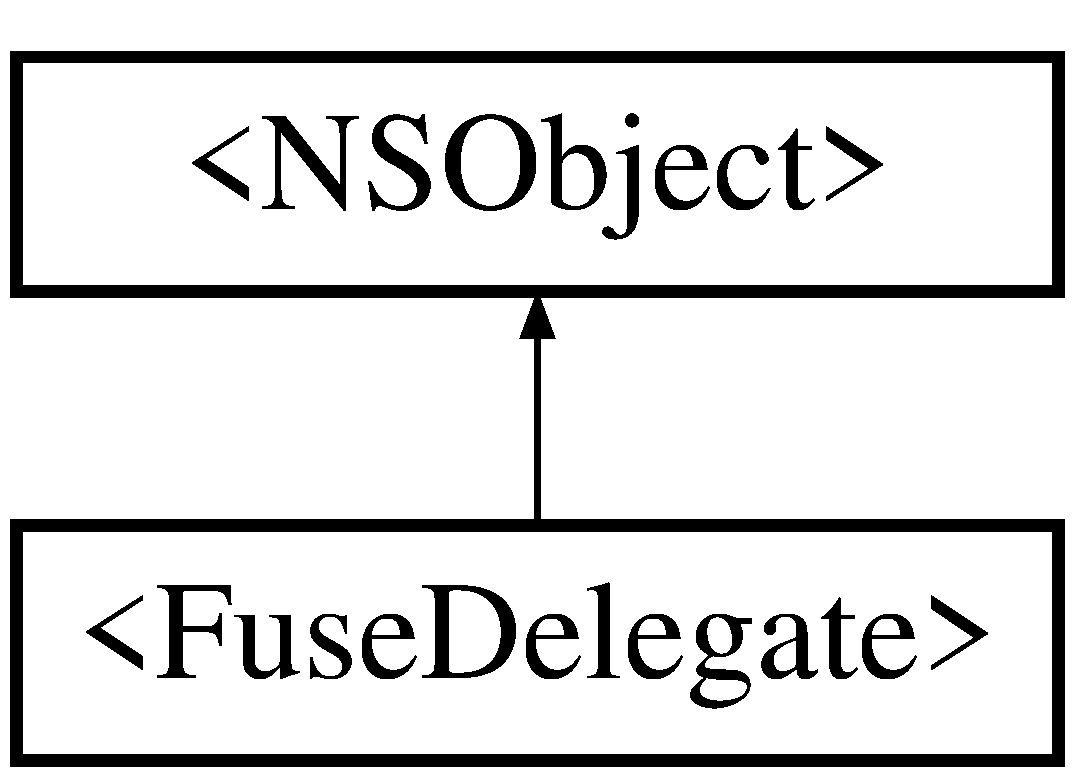
\includegraphics[height=2.000000cm]{protocol_fuse_delegate-p}
\end{center}
\end{figure}
\subsection*{Instance Methods}
\begin{DoxyCompactItemize}
\item 
(void) -\/ \hyperlink{protocol_fuse_delegate-p_a4278f68e73dc20a7a24b331959a1872c}{session\+Start\+Received}
\begin{DoxyCompactList}\small\item\em This method indicates when the server has acknowledged that a session has been established by the client device. \end{DoxyCompactList}\item 
(void) -\/ \hyperlink{protocol_fuse_delegate-p_a24b19ff8cc73955c5cc3b84428b302b0}{session\+Login\+Error\+:}
\begin{DoxyCompactList}\small\item\em This method is invoked when an error has occurred when trying to start a session. \end{DoxyCompactList}\item 
(void) -\/ \hyperlink{protocol_fuse_delegate-p_a85c5468cf940315584698956edcbbdfd}{time\+Updated\+:}
\begin{DoxyCompactList}\small\item\em This method indicates that the server U\+T\+C time has been received by the client device. \end{DoxyCompactList}\item 
(void) -\/ \hyperlink{protocol_fuse_delegate-p_a54a18530604a7ceeb0e9419fc7fa3345}{account\+Login\+Complete\+:\+Account\+:}
\begin{DoxyCompactList}\small\item\em This method notifies the device that an account login request has been received by the server. \end{DoxyCompactList}\item 
(void) -\/ \hyperlink{protocol_fuse_delegate-p_a1c8b10d8ec200c9d2aed94c494109a86}{account\+:login\+Error\+:}
\begin{DoxyCompactList}\small\item\em This method notifies the device that an account login request has failed. \end{DoxyCompactList}\item 
(void) -\/ \hyperlink{protocol_fuse_delegate-p_afc6afbdf6a149756eb2dca5e0fd64b77}{notification\+Action\+:}
\begin{DoxyCompactList}\small\item\em This method indicates that an action should be taken as a result of a notification being closed. \end{DoxyCompactList}\item 
(void) -\/ \hyperlink{protocol_fuse_delegate-p_ac493f7599268adadcc22e7c508b4ba61}{notfication\+Will\+Close}
\begin{DoxyCompactList}\small\item\em This method indicates that a visible notification is being closed. \end{DoxyCompactList}\item 
(void) -\/ \hyperlink{protocol_fuse_delegate-p_a1da152418e0a5dc2c1b108f501c6e627}{game\+Configuration\+Received}
\begin{DoxyCompactList}\small\item\em This method indicates that the game configuration values have been received by the client. \end{DoxyCompactList}\item 
(void) -\/ \hyperlink{protocol_fuse_delegate-p_a5c1b86ecfdc9518f976d5ea96156b408}{friend\+Added\+:\+Error\+:}
\begin{DoxyCompactList}\small\item\em This method indicates the result of an addition of a friend to the Fuse friends list system. \end{DoxyCompactList}\item 
(void) -\/ \hyperlink{protocol_fuse_delegate-p_a94ed7e39378bb2ae24ecc9c941dd0218}{friend\+Removed\+:\+Error\+:}
\begin{DoxyCompactList}\small\item\em This method indicates the result of a removal of a friend to the Fuse friends list system. \end{DoxyCompactList}\item 
(void) -\/ \hyperlink{protocol_fuse_delegate-p_ab48f8ef85f4f32654af102c5fa09c4c1}{friend\+Accepted\+:\+Error\+:}
\begin{DoxyCompactList}\small\item\em This method indicates the result of a acceptance of a friend to the Fuse friends list system. \end{DoxyCompactList}\item 
(void) -\/ \hyperlink{protocol_fuse_delegate-p_a2bc3be54c0a0a4f3cee3e9e96501c5ce}{friend\+Rejected\+:\+Error\+:}
\begin{DoxyCompactList}\small\item\em This method indicates the result of a rejection of a friend to the Fuse friends list system. \end{DoxyCompactList}\item 
(void) -\/ \hyperlink{protocol_fuse_delegate-p_adb2a01d8912d54c4a05a675e10901f6e}{friends\+Migrated\+:\+Error\+:}
\begin{DoxyCompactList}\small\item\em This method indicates the result of a rejection of a request to migrate friends from one account to another. \end{DoxyCompactList}\item 
(void) -\/ \hyperlink{protocol_fuse_delegate-p_a4b29ca96b491f3ac8548a85983aa0cff}{friends\+List\+Updated\+:}
\begin{DoxyCompactList}\small\item\em This method indicates when the friends list on the client has been updated from the server. \end{DoxyCompactList}\item 
(void) -\/ \hyperlink{protocol_fuse_delegate-p_a071433b93b221cbab7c0f112903e4718}{friends\+List\+Error\+:}
\begin{DoxyCompactList}\small\item\em This method indicates when an error has occurred in fetching the friends list from the server. \end{DoxyCompactList}\item 
(void) -\/ \hyperlink{protocol_fuse_delegate-p_a74e3e8647db995888bdf94c64d5ad26b}{purchase\+Verification\+:\+Transaction\+I\+D\+:\+Original\+Transaction\+I\+D\+:}
\begin{DoxyCompactList}\small\item\em This method indicates whether the registered in-\/app purchase has been validated by Apple's servers. \end{DoxyCompactList}\item 
(void) -\/ \hyperlink{protocol_fuse_delegate-p_ad9af5fda0a2199ba2a9a2bafab2f4a82}{ad\+Availability\+Response\+:\+Error\+:}
\begin{DoxyCompactList}\small\item\em Callback response to a request to load for an ad in the Fuse system. \end{DoxyCompactList}\item 
(void) -\/ \hyperlink{protocol_fuse_delegate-p_a3e81f123e745af07c58156c154c13cdc}{rewarded\+Ad\+Complete\+With\+Object\+:}
\begin{DoxyCompactList}\small\item\em Callback to acknowledge a successful rewarded Video Watch. \end{DoxyCompactList}\item 
(void) -\/ \hyperlink{protocol_fuse_delegate-p_ad46a55d7852f92e7615ce5168141bc7a}{I\+A\+P\+Offer\+Accepted\+With\+Object\+:}
\begin{DoxyCompactList}\small\item\em Callback to acknowledge an iap offer was accepted. \end{DoxyCompactList}\item 
(void) -\/ \hyperlink{protocol_fuse_delegate-p_a9577824db67c469466bd720d0193273d}{virtual\+Goods\+Offer\+Accepted\+With\+Object\+:}
\begin{DoxyCompactList}\small\item\em Callback to acknowledge an virtual goods offer was accepted. \end{DoxyCompactList}\item 
(void) -\/ \hyperlink{protocol_fuse_delegate-p_a1513d7db889fcaa54d7248f441b74072}{ad\+Failed\+To\+Display}
\begin{DoxyCompactList}\small\item\em Callback to inform no ad was displayed from show\+Ad\+For\+Zone\+I\+D\+:with\+Options\+: call. \end{DoxyCompactList}\item 
(void) -\/ \hyperlink{protocol_fuse_delegate-p_a2d725902d1f6c4c19d3ce3b65d60052b}{handle\+Ad\+Click\+With\+U\+R\+L\+:}
\begin{DoxyCompactList}\small\item\em If implemented, Ad\+Rally ads will pass this callback including the click-\/through U\+R\+L back to the application. It is then the application's responsibility to present an age gate and continue with the click-\/through if appropriate. \end{DoxyCompactList}\item 
(void) -\/ \hyperlink{protocol_fuse_delegate-p_a88bd02eb971260468ac6f6052bdda28f}{ad\+Did\+Show\+:media\+Type\+:}
\begin{DoxyCompactList}\small\item\em Callback to inform ad Did show. \end{DoxyCompactList}\item 
(void) -\/ \hyperlink{protocol_fuse_delegate-p_aafc293cd46be3bd70eeb60971b961a51}{ad\+Will\+Close}
\begin{DoxyCompactList}\small\item\em Callback to indicates when control is being returned to the application. \end{DoxyCompactList}\end{DoxyCompactItemize}


\subsection{Detailed Description}
This is the Fuse S\+D\+K delegate. 

This delegate is optional. However, relevant information might be passed to an object registered as a \hyperlink{interface_fuse_s_d_k}{Fuse\+S\+D\+K} delegate (application specific). A $<$\hyperlink{protocol_fuse_delegate-p}{Fuse\+Delegate}$>$ is registered in \hyperlink{interface_fuse_s_d_k_adf7ed64a02b9540c9ded4b931ea4e400}{start\+Session\+:delegate\+:with\+Options\+: (\+Fuse\+S\+D\+K)}. 

\subsection{Method Documentation}
\hypertarget{protocol_fuse_delegate-p_a1c8b10d8ec200c9d2aed94c494109a86}{}\index{Fuse\+Delegate-\/p@{Fuse\+Delegate-\/p}!account\+:login\+Error\+:@{account\+:login\+Error\+:}}
\index{account\+:login\+Error\+:@{account\+:login\+Error\+:}!Fuse\+Delegate-\/p@{Fuse\+Delegate-\/p}}
\subsubsection[{account\+:login\+Error\+:}]{\setlength{\rightskip}{0pt plus 5cm}-\/ (void) account\+: 
\begin{DoxyParamCaption}
\item[{(N\+S\+String $\ast$)}]{\+\_\+account\+\_\+id}
\item[{loginError:(N\+S\+Error $\ast$)}]{\+\_\+error}
\end{DoxyParamCaption}
\hspace{0.3cm}{\ttfamily [optional]}}\label{protocol_fuse_delegate-p_a1c8b10d8ec200c9d2aed94c494109a86}


This method notifies the device that an account login request has failed. 

When a user logs in using one of the available \hyperlink{interface_fuse_s_d_k}{Fuse\+S\+D\+K} account method, for instance \hyperlink{interface_fuse_s_d_k_a02a3bc5562d4f6e50bac5339f4ac4046}{game\+Center\+Login\+: (\+Fuse\+S\+D\+K)}, the server will send the client a notification if there is any errors encountered. 
\begin{DoxyParams}{Parameters}
{\em \+\_\+error} & \mbox{[}N\+S\+Error$\ast$\mbox{]} The error value corresponding to a value in E\+Fuse\+Error \\
\hline
{\em \+\_\+account\+\_\+id} & \mbox{[}N\+S\+String$\ast$\mbox{]} The account I\+D of the user attempted to log in \\
\hline
\end{DoxyParams}
\begin{DoxySeeAlso}{See also}
\hyperlink{interface_fuse_s_d_k_a02a3bc5562d4f6e50bac5339f4ac4046}{+ game\+Center\+Login\+: (\+Fuse\+S\+D\+K)} for a sample login method 
\end{DoxySeeAlso}
\begin{DoxySince}{Since}
Fuse S\+D\+K version 1.\+29 
\end{DoxySince}
\hypertarget{protocol_fuse_delegate-p_a54a18530604a7ceeb0e9419fc7fa3345}{}\index{Fuse\+Delegate-\/p@{Fuse\+Delegate-\/p}!account\+Login\+Complete\+:\+Account\+:@{account\+Login\+Complete\+:\+Account\+:}}
\index{account\+Login\+Complete\+:\+Account\+:@{account\+Login\+Complete\+:\+Account\+:}!Fuse\+Delegate-\/p@{Fuse\+Delegate-\/p}}
\subsubsection[{account\+Login\+Complete\+:\+Account\+:}]{\setlength{\rightskip}{0pt plus 5cm}-\/ (void) account\+Login\+Complete\+: 
\begin{DoxyParamCaption}
\item[{(N\+S\+Number $\ast$)}]{\+\_\+type}
\item[{Account:(N\+S\+String $\ast$)}]{\+\_\+account\+\_\+id}
\end{DoxyParamCaption}
\hspace{0.3cm}{\ttfamily [optional]}}\label{protocol_fuse_delegate-p_a54a18530604a7ceeb0e9419fc7fa3345}


This method notifies the device that an account login request has been received by the server. 

When a user logs in using one of the available \hyperlink{interface_fuse_s_d_k}{Fuse\+S\+D\+K} account method, for instance \hyperlink{interface_fuse_s_d_k_a02a3bc5562d4f6e50bac5339f4ac4046}{game\+Center\+Login\+: (\+Fuse\+S\+D\+K)}, the server will send the client a notification once received. This is to prevent any action being taken by the client before this has been received. 
\begin{DoxyParams}{Parameters}
{\em \+\_\+type} & \mbox{[}(N\+S\+Number$\ast$\mbox{]} Account type \\
\hline
{\em \+\_\+account\+\_\+id} & \mbox{[}N\+S\+String$\ast$\mbox{]} The account I\+D of the user logged in \\
\hline
\end{DoxyParams}
\begin{DoxySeeAlso}{See also}
\hyperlink{interface_fuse_s_d_k_a02a3bc5562d4f6e50bac5339f4ac4046}{+ game\+Center\+Login\+: (\+Fuse\+S\+D\+K)} for a sample login method 
\end{DoxySeeAlso}
\hypertarget{protocol_fuse_delegate-p_ad9af5fda0a2199ba2a9a2bafab2f4a82}{}\index{Fuse\+Delegate-\/p@{Fuse\+Delegate-\/p}!ad\+Availability\+Response\+:\+Error\+:@{ad\+Availability\+Response\+:\+Error\+:}}
\index{ad\+Availability\+Response\+:\+Error\+:@{ad\+Availability\+Response\+:\+Error\+:}!Fuse\+Delegate-\/p@{Fuse\+Delegate-\/p}}
\subsubsection[{ad\+Availability\+Response\+:\+Error\+:}]{\setlength{\rightskip}{0pt plus 5cm}-\/ (void) ad\+Availability\+Response\+: 
\begin{DoxyParamCaption}
\item[{(N\+S\+Number $\ast$)}]{\+\_\+available}
\item[{Error:(N\+S\+Error $\ast$)}]{\+\_\+error}
\end{DoxyParamCaption}
\hspace{0.3cm}{\ttfamily [optional]}}\label{protocol_fuse_delegate-p_ad9af5fda0a2199ba2a9a2bafab2f4a82}


Callback response to a request to load for an ad in the Fuse system. 

As a result of the preload\+Ad\+For\+Zone\+I\+D\+: method, this method is invoked when the status of whether an ad is available is known. To handle this response\+:


\begin{DoxyCode}
-(void) adAvailabilityResponse:(NSNumber*)\_available Error:(NSError*)\_error
\{
   BOOL isAvailable = [\_available boolValue];
   \textcolor{keywordtype}{int} error = [\_error code];

   \textcolor{keywordflow}{if} (error != FUSE\_AD\_NO\_ERROR)
   \{
       \textcolor{comment}{// An error has occurred checking for the ad}
   \}
   \textcolor{keywordflow}{else}
   \{
       \textcolor{keywordflow}{if} (isAvailable)
       \{
           \textcolor{comment}{// An ad is available}
       \}
       \textcolor{keywordflow}{else}
       \{
           \textcolor{comment}{// An ad is not available}
       \}
   \}
\}
\end{DoxyCode}



\begin{DoxyParams}{Parameters}
{\em \+\_\+available} & \mbox{[}N\+S\+Error $\ast$\mbox{]} This indicates whether an ad is available (boolean) \\
\hline
{\em \+\_\+error} & \mbox{[}N\+S\+Error $\ast$\mbox{]} This indicates whether an error has occurred and corresponds to values in E\+Fuse\+Error \\
\hline
\end{DoxyParams}
\begin{DoxySeeAlso}{See also}
preload\+Ad\+For\+Zone\+I\+D for more information on how to invoke the process of loading an ad zone. 
\end{DoxySeeAlso}
\begin{DoxySince}{Since}
Fuse S\+D\+K version 1.\+26 
\end{DoxySince}
\hypertarget{protocol_fuse_delegate-p_a88bd02eb971260468ac6f6052bdda28f}{}\index{Fuse\+Delegate-\/p@{Fuse\+Delegate-\/p}!ad\+Did\+Show\+:media\+Type\+:@{ad\+Did\+Show\+:media\+Type\+:}}
\index{ad\+Did\+Show\+:media\+Type\+:@{ad\+Did\+Show\+:media\+Type\+:}!Fuse\+Delegate-\/p@{Fuse\+Delegate-\/p}}
\subsubsection[{ad\+Did\+Show\+:media\+Type\+:}]{\setlength{\rightskip}{0pt plus 5cm}-\/ (void) ad\+Did\+Show\+: 
\begin{DoxyParamCaption}
\item[{(N\+S\+Number $\ast$)}]{\+\_\+network\+I\+D}
\item[{mediaType:(N\+S\+Number $\ast$)}]{\+\_\+media\+Type}
\end{DoxyParamCaption}
\hspace{0.3cm}{\ttfamily [optional]}}\label{protocol_fuse_delegate-p_a88bd02eb971260468ac6f6052bdda28f}


Callback to inform ad Did show. 

\begin{DoxySeeAlso}{See also}
Fuse\+S\+D\+K\+::show\+Ad\+For\+Zone\+I\+D\+:with\+Options\+: 
\end{DoxySeeAlso}
\begin{DoxySince}{Since}
Fuse S\+D\+K version 2.\+2.\+1 
\end{DoxySince}
\hypertarget{protocol_fuse_delegate-p_a1513d7db889fcaa54d7248f441b74072}{}\index{Fuse\+Delegate-\/p@{Fuse\+Delegate-\/p}!ad\+Failed\+To\+Display@{ad\+Failed\+To\+Display}}
\index{ad\+Failed\+To\+Display@{ad\+Failed\+To\+Display}!Fuse\+Delegate-\/p@{Fuse\+Delegate-\/p}}
\subsubsection[{ad\+Failed\+To\+Display}]{\setlength{\rightskip}{0pt plus 5cm}-\/ (void) ad\+Failed\+To\+Display 
\begin{DoxyParamCaption}
{}
\end{DoxyParamCaption}
\hspace{0.3cm}{\ttfamily [optional]}}\label{protocol_fuse_delegate-p_a1513d7db889fcaa54d7248f441b74072}


Callback to inform no ad was displayed from show\+Ad\+For\+Zone\+I\+D\+:with\+Options\+: call. 

\begin{DoxySeeAlso}{See also}
Fshow\+Ad\+For\+Zone\+I\+D\+:with\+Options\+: 
\end{DoxySeeAlso}
\begin{DoxySince}{Since}
Fuse S\+D\+K version 2.\+0.\+0 
\end{DoxySince}
\hypertarget{protocol_fuse_delegate-p_aafc293cd46be3bd70eeb60971b961a51}{}\index{Fuse\+Delegate-\/p@{Fuse\+Delegate-\/p}!ad\+Will\+Close@{ad\+Will\+Close}}
\index{ad\+Will\+Close@{ad\+Will\+Close}!Fuse\+Delegate-\/p@{Fuse\+Delegate-\/p}}
\subsubsection[{ad\+Will\+Close}]{\setlength{\rightskip}{0pt plus 5cm}-\/ (void) ad\+Will\+Close 
\begin{DoxyParamCaption}
{}
\end{DoxyParamCaption}
\hspace{0.3cm}{\ttfamily [required]}}\label{protocol_fuse_delegate-p_aafc293cd46be3bd70eeb60971b961a51}


Callback to indicates when control is being returned to the application. 

When an ad is being dismissed by the user and control is to be returned to the application, this method will be called. Once called, the application can continue execution of the user flow or application. \begin{DoxySeeAlso}{See also}
Fuse\+S\+D\+K\+::show\+Ad\+For\+Zone\+I\+D\+:with\+Options\+: for more information on displaying an ad with a $<$\hyperlink{protocol_fuse_delegate-p}{Fuse\+Delegate}$>$ 
\end{DoxySeeAlso}
\begin{DoxySince}{Since}
\hyperlink{interface_fuse_s_d_k}{Fuse\+S\+D\+K} version 1.\+12 
\end{DoxySince}
\hypertarget{protocol_fuse_delegate-p_ab48f8ef85f4f32654af102c5fa09c4c1}{}\index{Fuse\+Delegate-\/p@{Fuse\+Delegate-\/p}!friend\+Accepted\+:\+Error\+:@{friend\+Accepted\+:\+Error\+:}}
\index{friend\+Accepted\+:\+Error\+:@{friend\+Accepted\+:\+Error\+:}!Fuse\+Delegate-\/p@{Fuse\+Delegate-\/p}}
\subsubsection[{friend\+Accepted\+:\+Error\+:}]{\setlength{\rightskip}{0pt plus 5cm}-\/ (void) friend\+Accepted\+: 
\begin{DoxyParamCaption}
\item[{(N\+S\+String $\ast$)}]{\+\_\+fuse\+\_\+id}
\item[{Error:(N\+S\+Error $\ast$)}]{\+\_\+error}
\end{DoxyParamCaption}
\hspace{0.3cm}{\ttfamily [optional]}}\label{protocol_fuse_delegate-p_ab48f8ef85f4f32654af102c5fa09c4c1}


This method indicates the result of a acceptance of a friend to the Fuse friends list system. 

This method is optional, and only needs to be handled if the application needs to respond to errors in accepting friends. An example implementation would be\+:


\begin{DoxyCode}
-(void) friendAccepted:(NSString*)\_fuse\_id Error:(NSError*)\_error
\{
   \textcolor{keywordflow}{if} ([\_error intValue] == FUSE\_ACCEPT\_FRIEND\_NO\_ERROR)
   \{
       \textcolor{comment}{// no error has occurred in accepting a friend}
   \}
   \textcolor{keywordflow}{else}
   \{
       \textcolor{comment}{// an error has occurred}
   \}
\}
\end{DoxyCode}



\begin{DoxyParams}{Parameters}
{\em \+\_\+fuse\+\_\+id} & \mbox{[}N\+S\+String$\ast$\mbox{]} The fuse I\+D of the account for which the friend was accepted \\
\hline
{\em \+\_\+error} & \mbox{[}int\mbox{]} The error value corresponding to the a value in E\+Fuse\+Error \\
\hline
\end{DoxyParams}
\begin{DoxySeeAlso}{See also}
E\+Fuse\+Error for all possible error codes 

\hyperlink{interface_fuse_s_d_k_ae93cfa17f5b00ab1d28c53a8577c1af0}{+ accept\+Friend\+: (\+Fuse\+S\+D\+K)} for more information on accepting a friend 
\end{DoxySeeAlso}
\begin{DoxySince}{Since}
Fuse S\+D\+K version 1.\+22 
\end{DoxySince}
\hypertarget{protocol_fuse_delegate-p_a5c1b86ecfdc9518f976d5ea96156b408}{}\index{Fuse\+Delegate-\/p@{Fuse\+Delegate-\/p}!friend\+Added\+:\+Error\+:@{friend\+Added\+:\+Error\+:}}
\index{friend\+Added\+:\+Error\+:@{friend\+Added\+:\+Error\+:}!Fuse\+Delegate-\/p@{Fuse\+Delegate-\/p}}
\subsubsection[{friend\+Added\+:\+Error\+:}]{\setlength{\rightskip}{0pt plus 5cm}-\/ (void) friend\+Added\+: 
\begin{DoxyParamCaption}
\item[{(N\+S\+String $\ast$)}]{\+\_\+fuse\+\_\+id}
\item[{Error:(N\+S\+Error $\ast$)}]{\+\_\+error}
\end{DoxyParamCaption}
\hspace{0.3cm}{\ttfamily [optional]}}\label{protocol_fuse_delegate-p_a5c1b86ecfdc9518f976d5ea96156b408}


This method indicates the result of an addition of a friend to the Fuse friends list system. 

This method is optional, and only needs to be handled if the application needs to respond to errors in inviting friends. An example implementation would be\+:


\begin{DoxyCode}
-(void) friendAdded:(NSString*)\_fuse\_id Error:(NSError*)\_error
\{
   \textcolor{keywordflow}{if} (\_error == nil)
   \{
       \textcolor{comment}{// no error has occurred in adding a friend}
   \}
   \textcolor{keywordflow}{else}
   \{
       \textcolor{comment}{// an error has occurred}
   \}
\}
\end{DoxyCode}



\begin{DoxyParams}{Parameters}
{\em \+\_\+fuse\+\_\+id} & \mbox{[}N\+S\+String$\ast$\mbox{]} The fuse I\+D of the account for which the friend was added to \\
\hline
{\em \+\_\+error} & \mbox{[}int\mbox{]} The error value corresponding to the a value in E\+Fuse\+Error \\
\hline
\end{DoxyParams}
\begin{DoxySeeAlso}{See also}
E\+Fuse\+Error for all possible error codes 

\hyperlink{interface_fuse_s_d_k_a92b5888d1e5dafe2ab2a76fda44be4d8}{+ add\+Friend\+: (\+Fuse\+S\+D\+K)} for more information on adding a friend 
\end{DoxySeeAlso}
\begin{DoxySince}{Since}
Fuse S\+D\+K version 1.\+22 
\end{DoxySince}
\hypertarget{protocol_fuse_delegate-p_a2bc3be54c0a0a4f3cee3e9e96501c5ce}{}\index{Fuse\+Delegate-\/p@{Fuse\+Delegate-\/p}!friend\+Rejected\+:\+Error\+:@{friend\+Rejected\+:\+Error\+:}}
\index{friend\+Rejected\+:\+Error\+:@{friend\+Rejected\+:\+Error\+:}!Fuse\+Delegate-\/p@{Fuse\+Delegate-\/p}}
\subsubsection[{friend\+Rejected\+:\+Error\+:}]{\setlength{\rightskip}{0pt plus 5cm}-\/ (void) friend\+Rejected\+: 
\begin{DoxyParamCaption}
\item[{(N\+S\+String $\ast$)}]{\+\_\+fuse\+\_\+id}
\item[{Error:(N\+S\+Error $\ast$)}]{\+\_\+error}
\end{DoxyParamCaption}
\hspace{0.3cm}{\ttfamily [optional]}}\label{protocol_fuse_delegate-p_a2bc3be54c0a0a4f3cee3e9e96501c5ce}


This method indicates the result of a rejection of a friend to the Fuse friends list system. 

This method is optional, and only needs to be handled if the application needs to respond to errors in rejecting friends. An example implementation would be\+:


\begin{DoxyCode}
-(void) friendRejected:(NSString*)\_fuse\_id Error:(NSError*)\_error
\{
   \textcolor{keywordflow}{if} ([\_error intValue] == FUSE\_REJECT\_FRIEND\_NO\_ERROR)
   \{
       \textcolor{comment}{// no error has occurred in accepting a friend}
   \}
   \textcolor{keywordflow}{else}
   \{
       \textcolor{comment}{// an error has occurred}
   \}
\}
\end{DoxyCode}



\begin{DoxyParams}{Parameters}
{\em \+\_\+fuse\+\_\+id} & \mbox{[}N\+S\+String$\ast$\mbox{]} The fuse I\+D of the account for which the friend was rejected \\
\hline
{\em \+\_\+error} & \mbox{[}int\mbox{]} The error value corresponding to the a value in E\+Fuse\+Error \\
\hline
\end{DoxyParams}
\begin{DoxySeeAlso}{See also}
E\+Fuse\+Error for all possible error codes 

\hyperlink{interface_fuse_s_d_k_a8af1416799fd2922db49ed1de406f537}{+ reject\+Friend\+: (\+Fuse\+S\+D\+K)} for more information on rejecting a friend 
\end{DoxySeeAlso}
\begin{DoxySince}{Since}
Fuse S\+D\+K version 1.\+22 
\end{DoxySince}
\hypertarget{protocol_fuse_delegate-p_a94ed7e39378bb2ae24ecc9c941dd0218}{}\index{Fuse\+Delegate-\/p@{Fuse\+Delegate-\/p}!friend\+Removed\+:\+Error\+:@{friend\+Removed\+:\+Error\+:}}
\index{friend\+Removed\+:\+Error\+:@{friend\+Removed\+:\+Error\+:}!Fuse\+Delegate-\/p@{Fuse\+Delegate-\/p}}
\subsubsection[{friend\+Removed\+:\+Error\+:}]{\setlength{\rightskip}{0pt plus 5cm}-\/ (void) friend\+Removed\+: 
\begin{DoxyParamCaption}
\item[{(N\+S\+String $\ast$)}]{\+\_\+fuse\+\_\+id}
\item[{Error:(N\+S\+Error $\ast$)}]{\+\_\+error}
\end{DoxyParamCaption}
\hspace{0.3cm}{\ttfamily [optional]}}\label{protocol_fuse_delegate-p_a94ed7e39378bb2ae24ecc9c941dd0218}


This method indicates the result of a removal of a friend to the Fuse friends list system. 

This method is optional, and only needs to be handled if the application needs to respond to errors in removing friends. An example implementation would be\+:


\begin{DoxyCode}
-(void) friendRemoved:(NSString*)\_fuse\_id Error:(NSError*)\_error
\{
   \textcolor{keywordflow}{if} ([\_error intValue] == FUSE\_REMOVE\_FRIEND\_NO\_ERROR)
   \{
       \textcolor{comment}{// no error has occurred in removing a friend}
   \}
   \textcolor{keywordflow}{else}
   \{
       \textcolor{comment}{// an error has occurred}
   \}
\}
\end{DoxyCode}



\begin{DoxyParams}{Parameters}
{\em \+\_\+fuse\+\_\+id} & \mbox{[}N\+S\+String$\ast$\mbox{]} The fuse I\+D of the account for which the friend was removed \\
\hline
{\em \+\_\+error} & \mbox{[}int\mbox{]} The error value corresponding to the a value in E\+Fuse\+Error \\
\hline
\end{DoxyParams}
\begin{DoxySeeAlso}{See also}
E\+Fuse\+Error for all possible error codes 

\hyperlink{interface_fuse_s_d_k_a1556fd18ab2ae7f062c9d2ebbe2498fc}{+ remove\+Friend\+: (\+Fuse\+S\+D\+K)} for more information on removing a friend 
\end{DoxySeeAlso}
\begin{DoxySince}{Since}
Fuse S\+D\+K version 1.\+22 
\end{DoxySince}
\hypertarget{protocol_fuse_delegate-p_a071433b93b221cbab7c0f112903e4718}{}\index{Fuse\+Delegate-\/p@{Fuse\+Delegate-\/p}!friends\+List\+Error\+:@{friends\+List\+Error\+:}}
\index{friends\+List\+Error\+:@{friends\+List\+Error\+:}!Fuse\+Delegate-\/p@{Fuse\+Delegate-\/p}}
\subsubsection[{friends\+List\+Error\+:}]{\setlength{\rightskip}{0pt plus 5cm}-\/ (void) friends\+List\+Error\+: 
\begin{DoxyParamCaption}
\item[{(N\+S\+Error $\ast$)}]{\+\_\+error}
\end{DoxyParamCaption}
\hspace{0.3cm}{\ttfamily [optional]}}\label{protocol_fuse_delegate-p_a071433b93b221cbab7c0f112903e4718}


This method indicates when an error has occurred in fetching the friends list from the server. 

This method is a result of an error originating from the invocation of \hyperlink{interface_fuse_s_d_k_a11a92658dca5be9d79ca19a66bafb91e}{update\+Friends\+List\+From\+Server (\+Fuse\+S\+D\+K)} and indicates an error has occurred somewhere in the process.


\begin{DoxyCode}
-(void) friendsListError:(NSError*)\_error
\{
   \textcolor{keywordflow}{if} ([\_error intValue] != FUSE\_FRIENDS\_LIST\_NO\_ERROR)
   \{
       \textcolor{comment}{// An error has occurred}
   \}
\}
\end{DoxyCode}



\begin{DoxyParams}{Parameters}
{\em \+\_\+error} & \mbox{[}int\mbox{]} The error value corresponding to the a value in E\+Fuse\+Error \\
\hline
\end{DoxyParams}
\begin{DoxySeeAlso}{See also}
\hyperlink{interface_fuse_s_d_k_a11a92658dca5be9d79ca19a66bafb91e}{+ update\+Friends\+List\+From\+Server (\+Fuse\+S\+D\+K)} or more information on requesting the friends list from the server 
\end{DoxySeeAlso}
\begin{DoxySince}{Since}
Fuse S\+D\+K version 1.\+22 
\end{DoxySince}
\hypertarget{protocol_fuse_delegate-p_a4b29ca96b491f3ac8548a85983aa0cff}{}\index{Fuse\+Delegate-\/p@{Fuse\+Delegate-\/p}!friends\+List\+Updated\+:@{friends\+List\+Updated\+:}}
\index{friends\+List\+Updated\+:@{friends\+List\+Updated\+:}!Fuse\+Delegate-\/p@{Fuse\+Delegate-\/p}}
\subsubsection[{friends\+List\+Updated\+:}]{\setlength{\rightskip}{0pt plus 5cm}-\/ (void) friends\+List\+Updated\+: 
\begin{DoxyParamCaption}
\item[{(N\+S\+Dictionary $\ast$)}]{\+\_\+friends\+List}
\end{DoxyParamCaption}
\hspace{0.3cm}{\ttfamily [optional]}}\label{protocol_fuse_delegate-p_a4b29ca96b491f3ac8548a85983aa0cff}


This method indicates when the friends list on the client has been updated from the server. 

Either on the first fetch or subsequent updates of the friends list, this method is called every time the friends list is updated on the client. A friends list is requested from the server using \hyperlink{interface_fuse_s_d_k_a11a92658dca5be9d79ca19a66bafb91e}{update\+Friends\+List\+From\+Server (\+Fuse\+S\+D\+K)} and the process invokes this method with a dictionary of friends when complete. A sample implementation would be\+:


\begin{DoxyCode}
-(void) friendsListUpdated:(NSDictionary*)\_friendsList
\{
   \textcolor{comment}{// The friends list has returned to the device}

   \textcolor{comment}{// sample code to parse the dictionary}
   NSArray *fuse\_ids = [\_friendsList allKeys];

   \textcolor{keywordflow}{for} (\textcolor{keywordtype}{int} i = 0; i < [fuse\_ids count]; i++)
   \{
       NSString *fuse\_id = [fuse\_ids objectAtIndex:i];

       NSDictionary *friendEntry = (NSDictionary*)[\_friendsList objectForKey:fuse\_id];

       NSLog(\textcolor{stringliteral}{@"Friend is Pending: %d"}, [[friendEntry objectForKey:\textcolor{stringliteral}{@"pending"}] intValue]);
       NSLog(\textcolor{stringliteral}{@"Friend Alias: %@"}, [friendEntry objectForKey:\textcolor{stringliteral}{@"alias"}]);
       NSLog(\textcolor{stringliteral}{@"Friend Fuse ID: %@"}, [friendEntry objectForKey:\textcolor{stringliteral}{@"fuse\_id"}]);
   \}
\}
\end{DoxyCode}



\begin{DoxyParams}{Parameters}
{\em \+\_\+friends\+List} & \\
\hline
\end{DoxyParams}
\begin{DoxySeeAlso}{See also}
\hyperlink{interface_fuse_s_d_k_a11a92658dca5be9d79ca19a66bafb91e}{+ update\+Friends\+List\+From\+Server (\+Fuse\+S\+D\+K)} or more information on requesting the friends list from the server 

\hyperlink{interface_fuse_s_d_k_a31d609ce39be3e6eda04fd32d8036e95}{+ get\+Friends\+List (\+Fuse\+S\+D\+K)} for more information on requesting the local copy of the friends list 

\hyperlink{protocol_fuse_delegate-p_a071433b93b221cbab7c0f112903e4718}{-\/ friends\+List\+Error\+:} to handle errors involved in requesting the friends list from the Fuse server 
\end{DoxySeeAlso}
\begin{DoxySince}{Since}
Fuse S\+D\+K version 1.\+22 
\end{DoxySince}
\hypertarget{protocol_fuse_delegate-p_adb2a01d8912d54c4a05a675e10901f6e}{}\index{Fuse\+Delegate-\/p@{Fuse\+Delegate-\/p}!friends\+Migrated\+:\+Error\+:@{friends\+Migrated\+:\+Error\+:}}
\index{friends\+Migrated\+:\+Error\+:@{friends\+Migrated\+:\+Error\+:}!Fuse\+Delegate-\/p@{Fuse\+Delegate-\/p}}
\subsubsection[{friends\+Migrated\+:\+Error\+:}]{\setlength{\rightskip}{0pt plus 5cm}-\/ (void) friends\+Migrated\+: 
\begin{DoxyParamCaption}
\item[{(N\+S\+String $\ast$)}]{\+\_\+fuse\+\_\+id}
\item[{Error:(N\+S\+Error $\ast$)}]{\+\_\+error}
\end{DoxyParamCaption}
\hspace{0.3cm}{\ttfamily [optional]}}\label{protocol_fuse_delegate-p_adb2a01d8912d54c4a05a675e10901f6e}


This method indicates the result of a rejection of a request to migrate friends from one account to another. 

This method is optional, and only needs to be handled if the application needs to respond to errors in migrating friends. An example implementation would be\+:


\begin{DoxyCode}
-(void) friendsMigrated:(NSString*)\_fuse\_id Error:(NSError*)\_error
\{
    \textcolor{keywordflow}{if} ([\_error intValue] == FUSE\_MIGRATE\_FRIENDS\_NO\_ERROR)
    \{
        \textcolor{comment}{// no error has occurred in accepting a friend}
    \}
    \textcolor{keywordflow}{else}
    \{
        \textcolor{comment}{// an error has occurred}
    \}
\}
\end{DoxyCode}



\begin{DoxyParams}{Parameters}
{\em \+\_\+fuse\+\_\+id} & \mbox{[}N\+S\+String$\ast$\mbox{]} The fuse I\+D of the account for which the friend's are to be migrated from \\
\hline
{\em \+\_\+error} & \mbox{[}int\mbox{]} The error value corresponding to the a value in E\+Fuse\+Error \\
\hline
\end{DoxyParams}
\begin{DoxySeeAlso}{See also}
E\+Fuse\+Error for all possible error codes 

\hyperlink{interface_fuse_s_d_k_a199e36abe741ecdf8062d1afddc6e146}{+ migrate\+Friends\+: (\+Fuse\+S\+D\+K)} for more information on migrating friends 
\end{DoxySeeAlso}
\begin{DoxySince}{Since}
Fuse S\+D\+K version 1.\+34.\+1 
\end{DoxySince}
\hypertarget{protocol_fuse_delegate-p_a1da152418e0a5dc2c1b108f501c6e627}{}\index{Fuse\+Delegate-\/p@{Fuse\+Delegate-\/p}!game\+Configuration\+Received@{game\+Configuration\+Received}}
\index{game\+Configuration\+Received@{game\+Configuration\+Received}!Fuse\+Delegate-\/p@{Fuse\+Delegate-\/p}}
\subsubsection[{game\+Configuration\+Received}]{\setlength{\rightskip}{0pt plus 5cm}-\/ (void) game\+Configuration\+Received 
\begin{DoxyParamCaption}
{}
\end{DoxyParamCaption}
\hspace{0.3cm}{\ttfamily [optional]}}\label{protocol_fuse_delegate-p_a1da152418e0a5dc2c1b108f501c6e627}


This method indicates that the game configuration values have been received by the client. 

To avoid polling values before they are sent from the server, this callback can be used to determine when they are valid. These values are update when a user starts or resumes a session. \begin{DoxySeeAlso}{See also}
\hyperlink{interface_fuse_s_d_k_ab29213306801eba35d922754a5efa1b0}{+ get\+Game\+Configuration\+Value\+: (\+Fuse\+S\+D\+K)} for more information on reading game configuration values once valid 
\end{DoxySeeAlso}
\hypertarget{protocol_fuse_delegate-p_a2d725902d1f6c4c19d3ce3b65d60052b}{}\index{Fuse\+Delegate-\/p@{Fuse\+Delegate-\/p}!handle\+Ad\+Click\+With\+U\+R\+L\+:@{handle\+Ad\+Click\+With\+U\+R\+L\+:}}
\index{handle\+Ad\+Click\+With\+U\+R\+L\+:@{handle\+Ad\+Click\+With\+U\+R\+L\+:}!Fuse\+Delegate-\/p@{Fuse\+Delegate-\/p}}
\subsubsection[{handle\+Ad\+Click\+With\+U\+R\+L\+:}]{\setlength{\rightskip}{0pt plus 5cm}-\/ (void) handle\+Ad\+Click\+With\+U\+R\+L\+: 
\begin{DoxyParamCaption}
\item[{(N\+S\+U\+R\+L $\ast$)}]{\+\_\+url}
\end{DoxyParamCaption}
\hspace{0.3cm}{\ttfamily [optional]}}\label{protocol_fuse_delegate-p_a2d725902d1f6c4c19d3ce3b65d60052b}


If implemented, Ad\+Rally ads will pass this callback including the click-\/through U\+R\+L back to the application. It is then the application's responsibility to present an age gate and continue with the click-\/through if appropriate. 

In Order to use this Delegate Call, The option k\+Fuse\+S\+D\+K\+Option\+Key\+\_\+\+Handle\+Ad\+U\+R\+Ls must be passed with the value  \begin{DoxySince}{Since}
Fuse S\+D\+K version 2.\+1.\+0 
\end{DoxySince}
\hypertarget{protocol_fuse_delegate-p_ad46a55d7852f92e7615ce5168141bc7a}{}\index{Fuse\+Delegate-\/p@{Fuse\+Delegate-\/p}!I\+A\+P\+Offer\+Accepted\+With\+Object\+:@{I\+A\+P\+Offer\+Accepted\+With\+Object\+:}}
\index{I\+A\+P\+Offer\+Accepted\+With\+Object\+:@{I\+A\+P\+Offer\+Accepted\+With\+Object\+:}!Fuse\+Delegate-\/p@{Fuse\+Delegate-\/p}}
\subsubsection[{I\+A\+P\+Offer\+Accepted\+With\+Object\+:}]{\setlength{\rightskip}{0pt plus 5cm}-\/ (void) I\+A\+P\+Offer\+Accepted\+With\+Object\+: 
\begin{DoxyParamCaption}
\item[{({\bf Fuse\+I\+A\+P\+Offer\+Object} $\ast$)}]{\+\_\+offer}
\end{DoxyParamCaption}
\hspace{0.3cm}{\ttfamily [optional]}}\label{protocol_fuse_delegate-p_ad46a55d7852f92e7615ce5168141bc7a}


Callback to acknowledge an iap offer was accepted. 


\begin{DoxyParams}{Parameters}
{\em \+\_\+offer} & (Fuse\+I\+A\+P\+Offer\+Object$\ast$) Object containing offer information \\
\hline
\end{DoxyParams}
\begin{DoxySeeAlso}{See also}
\hyperlink{interface_fuse_i_a_p_offer_object}{Fuse\+I\+A\+P\+Offer\+Object} in Fuse\+S\+D\+K\+Defintions.\+h for more information 
\end{DoxySeeAlso}
\begin{DoxySince}{Since}
Fuse S\+D\+K version 2.\+0.\+0 
\end{DoxySince}
\hypertarget{protocol_fuse_delegate-p_ac493f7599268adadcc22e7c508b4ba61}{}\index{Fuse\+Delegate-\/p@{Fuse\+Delegate-\/p}!notfication\+Will\+Close@{notfication\+Will\+Close}}
\index{notfication\+Will\+Close@{notfication\+Will\+Close}!Fuse\+Delegate-\/p@{Fuse\+Delegate-\/p}}
\subsubsection[{notfication\+Will\+Close}]{\setlength{\rightskip}{0pt plus 5cm}-\/ (void) notfication\+Will\+Close 
\begin{DoxyParamCaption}
{}
\end{DoxyParamCaption}
\hspace{0.3cm}{\ttfamily [optional]}}\label{protocol_fuse_delegate-p_ac493f7599268adadcc22e7c508b4ba61}


This method indicates that a visible notification is being closed. 

\begin{DoxySeeAlso}{See also}
\hyperlink{interface_fuse_s_d_k_a279e4cb8e95a3e78197761156a7de50d}{+ display\+Notifications (\+Fuse\+S\+D\+K)} for more information on displaying in-\/game notifications 
\end{DoxySeeAlso}
\hypertarget{protocol_fuse_delegate-p_afc6afbdf6a149756eb2dca5e0fd64b77}{}\index{Fuse\+Delegate-\/p@{Fuse\+Delegate-\/p}!notification\+Action\+:@{notification\+Action\+:}}
\index{notification\+Action\+:@{notification\+Action\+:}!Fuse\+Delegate-\/p@{Fuse\+Delegate-\/p}}
\subsubsection[{notification\+Action\+:}]{\setlength{\rightskip}{0pt plus 5cm}-\/ (void) notification\+Action\+: 
\begin{DoxyParamCaption}
\item[{(N\+S\+String $\ast$)}]{\+\_\+action}
\end{DoxyParamCaption}
\hspace{0.3cm}{\ttfamily [optional]}}\label{protocol_fuse_delegate-p_afc6afbdf6a149756eb2dca5e0fd64b77}


This method indicates that an action should be taken as a result of a notification being closed. 

To handle any possible action as a result of an in-\/game notification being displayed, a custom string can be configured as a part of the notification setup process in the Fuse dashboard. This string can be any value that is recognized by the application. For instance, a sample of this in action would be\+:


\begin{DoxyCode}
-(void) notificationAction:(NSString*)\_action
\{
   \textcolor{keywordflow}{if} ([\_action isEqualToString:\textcolor{stringliteral}{@"GO\_TO\_LEVEL\_2"}])
   \{
       \textcolor{comment}{// Take the user to level 2 for instance}
   \}
   \textcolor{keywordflow}{else} \textcolor{keywordflow}{if} ([\_action isEqualToString:\textcolor{stringliteral}{@"GO\_TO\_SALE"}])
   \{
       \textcolor{comment}{// Take the user to the sale section of your store}
   \}
\}
\end{DoxyCode}



\begin{DoxyParams}{Parameters}
{\em \+\_\+action} & \mbox{[}N\+S\+String$\ast$\mbox{]} The string value that indicates what action to take. Custom and application specific. \\
\hline
\end{DoxyParams}
\begin{DoxySeeAlso}{See also}
\hyperlink{interface_fuse_s_d_k_a279e4cb8e95a3e78197761156a7de50d}{+ display\+Notifications (\+Fuse\+S\+D\+K)} for more information on displaying in-\/game notifications 
\end{DoxySeeAlso}
\hypertarget{protocol_fuse_delegate-p_a74e3e8647db995888bdf94c64d5ad26b}{}\index{Fuse\+Delegate-\/p@{Fuse\+Delegate-\/p}!purchase\+Verification\+:\+Transaction\+I\+D\+:\+Original\+Transaction\+I\+D\+:@{purchase\+Verification\+:\+Transaction\+I\+D\+:\+Original\+Transaction\+I\+D\+:}}
\index{purchase\+Verification\+:\+Transaction\+I\+D\+:\+Original\+Transaction\+I\+D\+:@{purchase\+Verification\+:\+Transaction\+I\+D\+:\+Original\+Transaction\+I\+D\+:}!Fuse\+Delegate-\/p@{Fuse\+Delegate-\/p}}
\subsubsection[{purchase\+Verification\+:\+Transaction\+I\+D\+:\+Original\+Transaction\+I\+D\+:}]{\setlength{\rightskip}{0pt plus 5cm}-\/ (void) purchase\+Verification\+: 
\begin{DoxyParamCaption}
\item[{(N\+S\+Number $\ast$)}]{\+\_\+verified}
\item[{TransactionID:(N\+S\+String $\ast$)}]{\+\_\+tx\+\_\+id}
\item[{OriginalTransactionID:(N\+S\+String $\ast$)}]{\+\_\+o\+\_\+tx\+\_\+id}
\end{DoxyParamCaption}
\hspace{0.3cm}{\ttfamily [optional]}}\label{protocol_fuse_delegate-p_a74e3e8647db995888bdf94c64d5ad26b}


This method indicates whether the registered in-\/app purchase has been validated by Apple's servers. 

This method is optional can indicates via the \+\_\+verified bit if the in-\/app purchase was valid. The Fuse servers initiate communication with Apple's in-\/app purchase verification servers once a call to \hyperlink{interface_fuse_s_d_k_a2dd50722daab117889c396ff58fe7c27}{register\+In\+App\+Purchase\+: (\+Fuse\+S\+D\+K)} is invoked. This callback is the result of that process. If the \+\_\+validated bit comes back as a '1', it can be safely concluded that the purchase is definitely valid. However, if the bit comes back as '0', the purchase should only be treated as suspect as it is not definitive at this point whether it was invalid or an error occurred in the process.


\begin{DoxyCode}
-(void) purchaseVerification:(NSNumber*)\_verified TransactionID:(NSString*)\_tx\_id OriginalTransactionID:(
      NSString*)\_o\_tx\_id
\{
   BOOL is\_valid = [\_verified boolValue];

   \textcolor{keywordflow}{if} (is\_valid)
   \{
       \textcolor{comment}{// valid transaction}
   \}
   \textcolor{keywordflow}{else}
   \{
       \textcolor{comment}{// suspect transaction}
   \}
\}
\end{DoxyCode}



\begin{DoxyParams}{Parameters}
{\em \+\_\+verified} & \mbox{[}N\+S\+S\+Number$\ast$\mbox{]} This is the \+\_\+verified bit\+: 1 indicates that the transaction was valid. 0 indicates that the transaction should be treated with suspicion. \\
\hline
{\em \+\_\+tx\+\_\+id} & \mbox{[}N\+S\+String$\ast$\mbox{]} The transaction I\+D specified by Apple \\
\hline
{\em \+\_\+o\+\_\+tx\+\_\+id} & \mbox{[}N\+S\+String$\ast$\mbox{]} The original transaction I\+D specified by Apple (can be different than the transaction I\+D because the transaction could be a reinstatement of a previous purchase)\\
\hline
\end{DoxyParams}
\begin{DoxySeeAlso}{See also}
\href{https://developer.apple.com/library/ios/releasenotes/General/ValidateAppStoreReceipt/Chapters/ValidateRemotely.html}{\tt https\+://developer.\+apple.\+com/library/ios/releasenotes/\+General/\+Validate\+App\+Store\+Receipt/\+Chapters/\+Validate\+Remotely.\+html} For information how to collect Receipt when registering in app purchases 

\hyperlink{interface_fuse_s_d_k_a2dd50722daab117889c396ff58fe7c27}{+ register\+In\+App\+Purchase\+: (\+Fuse\+S\+D\+K)} for more information on how to invoke this process 
\end{DoxySeeAlso}
\hypertarget{protocol_fuse_delegate-p_a3e81f123e745af07c58156c154c13cdc}{}\index{Fuse\+Delegate-\/p@{Fuse\+Delegate-\/p}!rewarded\+Ad\+Complete\+With\+Object\+:@{rewarded\+Ad\+Complete\+With\+Object\+:}}
\index{rewarded\+Ad\+Complete\+With\+Object\+:@{rewarded\+Ad\+Complete\+With\+Object\+:}!Fuse\+Delegate-\/p@{Fuse\+Delegate-\/p}}
\subsubsection[{rewarded\+Ad\+Complete\+With\+Object\+:}]{\setlength{\rightskip}{0pt plus 5cm}-\/ (void) rewarded\+Ad\+Complete\+With\+Object\+: 
\begin{DoxyParamCaption}
\item[{({\bf Fuse\+Rewarded\+Object} $\ast$)}]{\+\_\+reward}
\end{DoxyParamCaption}
\hspace{0.3cm}{\ttfamily [optional]}}\label{protocol_fuse_delegate-p_a3e81f123e745af07c58156c154c13cdc}


Callback to acknowledge a successful rewarded Video Watch. 


\begin{DoxyParams}{Parameters}
{\em reward} & (Fuse\+Rewarded\+Object$\ast$) Object containing rewarded information \\
\hline
\end{DoxyParams}
\begin{DoxySeeAlso}{See also}
\hyperlink{interface_fuse_rewarded_object}{Fuse\+Rewarded\+Object} in Fuse\+S\+D\+K\+Defintions.\+h for more information 
\end{DoxySeeAlso}
\begin{DoxySince}{Since}
Fuse S\+D\+K version 2.\+0.\+0 
\end{DoxySince}
\hypertarget{protocol_fuse_delegate-p_a24b19ff8cc73955c5cc3b84428b302b0}{}\index{Fuse\+Delegate-\/p@{Fuse\+Delegate-\/p}!session\+Login\+Error\+:@{session\+Login\+Error\+:}}
\index{session\+Login\+Error\+:@{session\+Login\+Error\+:}!Fuse\+Delegate-\/p@{Fuse\+Delegate-\/p}}
\subsubsection[{session\+Login\+Error\+:}]{\setlength{\rightskip}{0pt plus 5cm}-\/ (void) session\+Login\+Error\+: 
\begin{DoxyParamCaption}
\item[{(N\+S\+Error $\ast$)}]{\+\_\+error}
\end{DoxyParamCaption}
}\label{protocol_fuse_delegate-p_a24b19ff8cc73955c5cc3b84428b302b0}


This method is invoked when an error has occurred when trying to start a session. 

To avoid cases where operations are continuing as if everything was being handled normally by the \hyperlink{interface_fuse_s_d_k}{Fuse\+S\+D\+K}, this can be listened to and actions taken as a result. This method is optional. 
\begin{DoxyParams}{Parameters}
{\em \+\_\+error} & \mbox{[}N\+S\+Error$\ast$\mbox{]} The error value corresponding to a value in E\+Fuse\+Error \\
\hline
\end{DoxyParams}
\begin{DoxySeeAlso}{See also}
\hyperlink{interface_fuse_s_d_k_adf7ed64a02b9540c9ded4b931ea4e400}{+ start\+Session\+:delegate\+:with\+Options\+: (\+Fuse\+S\+D\+K)} for more information on starting a session with a $<$\hyperlink{protocol_fuse_delegate-p}{Fuse\+Delegate}$>$ 

E\+Fuse\+Error for more information on all possible error values 
\end{DoxySeeAlso}
\hypertarget{protocol_fuse_delegate-p_a4278f68e73dc20a7a24b331959a1872c}{}\index{Fuse\+Delegate-\/p@{Fuse\+Delegate-\/p}!session\+Start\+Received@{session\+Start\+Received}}
\index{session\+Start\+Received@{session\+Start\+Received}!Fuse\+Delegate-\/p@{Fuse\+Delegate-\/p}}
\subsubsection[{session\+Start\+Received}]{\setlength{\rightskip}{0pt plus 5cm}-\/ (void) session\+Start\+Received 
\begin{DoxyParamCaption}
{}
\end{DoxyParamCaption}
}\label{protocol_fuse_delegate-p_a4278f68e73dc20a7a24b331959a1872c}


This method indicates when the server has acknowledged that a session has been established by the client device. 

When a delegate is registered with the \hyperlink{interface_fuse_s_d_k_adf7ed64a02b9540c9ded4b931ea4e400}{start\+Session\+:delegate\+:with\+Options\+: (\+Fuse\+S\+D\+K)} method, and the acknowledgement of the connection has been received, this method is invoked. This method is optional and is only intended to help in cases where this information is relevant to the application. \begin{DoxySeeAlso}{See also}
\hyperlink{interface_fuse_s_d_k_adf7ed64a02b9540c9ded4b931ea4e400}{+ start\+Session\+:delegate\+:with\+Options\+: (\+Fuse\+S\+D\+K)} for more information on starting a session with a $<$\hyperlink{protocol_fuse_delegate-p}{Fuse\+Delegate}$>$ 
\end{DoxySeeAlso}
\hypertarget{protocol_fuse_delegate-p_a85c5468cf940315584698956edcbbdfd}{}\index{Fuse\+Delegate-\/p@{Fuse\+Delegate-\/p}!time\+Updated\+:@{time\+Updated\+:}}
\index{time\+Updated\+:@{time\+Updated\+:}!Fuse\+Delegate-\/p@{Fuse\+Delegate-\/p}}
\subsubsection[{time\+Updated\+:}]{\setlength{\rightskip}{0pt plus 5cm}-\/ (void) time\+Updated\+: 
\begin{DoxyParamCaption}
\item[{(N\+S\+Number $\ast$)}]{\+\_\+utc\+Time\+Stamp}
\end{DoxyParamCaption}
\hspace{0.3cm}{\ttfamily [optional]}}\label{protocol_fuse_delegate-p_a85c5468cf940315584698956edcbbdfd}


This method indicates that the server U\+T\+C time has been received by the client device. 

This method can be called both as a result of \hyperlink{interface_fuse_s_d_k_a60de732b9ecb7bce2439517cc2ca1f71}{utc\+Time\+From\+Server (\+Fuse\+S\+D\+K)} or automatically after a time event has been sent from the Fuse system (generally only happens when a session is started or resumed). The time should only be treated a psuedo-\/accurate. There are delays in propagating the time from the server to the device.


\begin{DoxyCode}
-(void) timeUpdated:(NSNumber*)\_utcTimeStamp
\{
   \textcolor{keywordtype}{int} utc\_unix\_timestamp = [utcTimeStamp intValue];
\}
\end{DoxyCode}



\begin{DoxyParams}{Parameters}
{\em \+\_\+utc\+Time\+Stamp} & \mbox{[}int\mbox{]} \\
\hline
\end{DoxyParams}
\begin{DoxySeeAlso}{See also}
\hyperlink{interface_fuse_s_d_k_a60de732b9ecb7bce2439517cc2ca1f71}{+ utc\+Time\+From\+Server (\+Fuse\+S\+D\+K)} for more information on directly requesting the U\+T\+C time from the server 

\href{http://en.wikipedia.org/wiki/Unix_time}{\tt http\+://en.\+wikipedia.\+org/wiki/\+Unix\+\_\+time} for more information on Unix time 

\href{http://en.wikipedia.org/wiki/Coordinated_Universal_Time}{\tt http\+://en.\+wikipedia.\+org/wiki/\+Coordinated\+\_\+\+Universal\+\_\+\+Time} for more information on U\+T\+C time 
\end{DoxySeeAlso}
\hypertarget{protocol_fuse_delegate-p_a9577824db67c469466bd720d0193273d}{}\index{Fuse\+Delegate-\/p@{Fuse\+Delegate-\/p}!virtual\+Goods\+Offer\+Accepted\+With\+Object\+:@{virtual\+Goods\+Offer\+Accepted\+With\+Object\+:}}
\index{virtual\+Goods\+Offer\+Accepted\+With\+Object\+:@{virtual\+Goods\+Offer\+Accepted\+With\+Object\+:}!Fuse\+Delegate-\/p@{Fuse\+Delegate-\/p}}
\subsubsection[{virtual\+Goods\+Offer\+Accepted\+With\+Object\+:}]{\setlength{\rightskip}{0pt plus 5cm}-\/ (void) virtual\+Goods\+Offer\+Accepted\+With\+Object\+: 
\begin{DoxyParamCaption}
\item[{({\bf Fuse\+Virtual\+Goods\+Offer\+Object} $\ast$)}]{\+\_\+offer}
\end{DoxyParamCaption}
\hspace{0.3cm}{\ttfamily [optional]}}\label{protocol_fuse_delegate-p_a9577824db67c469466bd720d0193273d}


Callback to acknowledge an virtual goods offer was accepted. 


\begin{DoxyParams}{Parameters}
{\em \+\_\+offer} & (Fuse\+Virtual\+Goods\+Offer\+Object$\ast$) Object containing offer information \\
\hline
\end{DoxyParams}
\begin{DoxySeeAlso}{See also}
\hyperlink{interface_fuse_virtual_goods_offer_object}{Fuse\+Virtual\+Goods\+Offer\+Object} in Fuse\+S\+D\+K\+Defintions.\+h for more information 
\end{DoxySeeAlso}
\begin{DoxySince}{Since}
Fuse S\+D\+K version 2.\+0.\+0 
\end{DoxySince}


The documentation for this protocol was generated from the following file\+:\begin{DoxyCompactItemize}
\item 
/\+Users/buildmachine/buildmonkey/\+Fuse\+S\+D\+Ki\+O\+S-\/master/\+Code/\+Classes/\+Fuse\+S\+D\+K/Fuse\+S\+D\+K.\+h\end{DoxyCompactItemize}

\hypertarget{protocol_fuse_game_data_delegate-p}{}\section{$<$Fuse\+Game\+Data\+Delegate$>$ Protocol Reference}
\label{protocol_fuse_game_data_delegate-p}\index{$<$\+Fuse\+Game\+Data\+Delegate$>$@{$<$\+Fuse\+Game\+Data\+Delegate$>$}}


This is the game data delegate which receives notifications from getting and setting user data.  




{\ttfamily \#import $<$Fuse\+A\+P\+I.\+h$>$}

Inheritance diagram for $<$Fuse\+Game\+Data\+Delegate$>$\+:\begin{figure}[H]
\begin{center}
\leavevmode
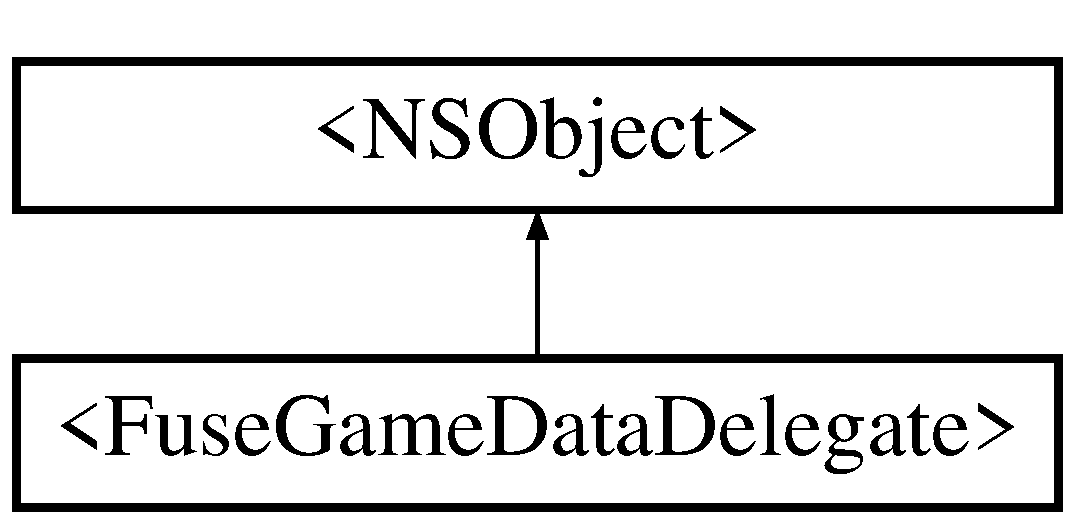
\includegraphics[height=2.000000cm]{protocol_fuse_game_data_delegate-p}
\end{center}
\end{figure}
\subsection*{Instance Methods}
\begin{DoxyCompactItemize}
\item 
(void) -\/ \hyperlink{protocol_fuse_game_data_delegate-p_a779286e74bd187861e72baa22c4a1c90}{game\+Data\+Received\+:\+For\+Key\+:\+Data\+:}
\begin{DoxyCompactList}\small\item\em This method is called when the request for game data has returned to the device. This method does not receieve the request I\+D in the callback, unlike game\+Data\+Received\+:\+For\+Key\+:\+Data\+:\+Request\+I\+D\+: which can be optionally used instead (if required). \end{DoxyCompactList}\item 
(void) -\/ \hyperlink{protocol_fuse_game_data_delegate-p_ad4381e7c5b070343b22d62a337ccd8a8}{game\+Data\+Received\+:\+For\+Key\+:\+Data\+:\+Request\+I\+D\+:}
\begin{DoxyCompactList}\small\item\em This method is called when the request for game data has returned to the device. \end{DoxyCompactList}\item 
(void) -\/ \hyperlink{protocol_fuse_game_data_delegate-p_ae30d8baf6c1114c83a39d1cb4bd8bdd0}{game\+Data\+Error\+:}
\begin{DoxyCompactList}\small\item\em This method indicates when an error has occurred when sending or receiving per-\/user game data information. \end{DoxyCompactList}\item 
(void) -\/ \hyperlink{protocol_fuse_game_data_delegate-p_ab2b869abbcd0fdb1ca5ccf4bddfb6f00}{game\+Data\+Error\+:\+Request\+I\+D\+:}
\begin{DoxyCompactList}\small\item\em This method indicates when an error has occurred when sending or receiving per-\/user game data information. \end{DoxyCompactList}\item 
(void) -\/ \hyperlink{protocol_fuse_game_data_delegate-p_a9888e6aaf263e84a9086e4e80fc01c15}{game\+Data\+Set\+Acknowledged\+:}
\begin{DoxyCompactList}\small\item\em This method indicates the server has acknowledged a save of per-\/user game data. \end{DoxyCompactList}\end{DoxyCompactItemize}


\subsection{Detailed Description}
This is the game data delegate which receives notifications from getting and setting user data. 

Handles all notification events involved in sending and receiving per-\/user game data. This is not required unless the methods \hyperlink{interface_fuse_a_p_i_a3da637831ec4d7dcd4d45cd7c547cd6a}{set\+Game\+Data\+:\+Delegate\+: (\+Fuse\+A\+P\+I)} or \hyperlink{interface_fuse_a_p_i_a45365af9ff3e5defee7e63de10374ad1}{get\+Game\+Data\+:\+Delegate\+: (\+Fuse\+A\+P\+I)} (or others of the same family) are implemented 

\subsection{Method Documentation}
\hypertarget{protocol_fuse_game_data_delegate-p_ae30d8baf6c1114c83a39d1cb4bd8bdd0}{}\index{Fuse\+Game\+Data\+Delegate-\/p@{Fuse\+Game\+Data\+Delegate-\/p}!game\+Data\+Error\+:@{game\+Data\+Error\+:}}
\index{game\+Data\+Error\+:@{game\+Data\+Error\+:}!Fuse\+Game\+Data\+Delegate-\/p@{Fuse\+Game\+Data\+Delegate-\/p}}
\subsubsection[{game\+Data\+Error\+:}]{\setlength{\rightskip}{0pt plus 5cm}-\/ (void) game\+Data\+Error\+: 
\begin{DoxyParamCaption}
\item[{(N\+S\+Number $\ast$)}]{\+\_\+error}
\end{DoxyParamCaption}
\hspace{0.3cm}{\ttfamily [optional]}}\label{protocol_fuse_game_data_delegate-p_ae30d8baf6c1114c83a39d1cb4bd8bdd0}


This method indicates when an error has occurred when sending or receiving per-\/user game data information. 

When an error occurs when trying to set or retrieve game data, this method will be thrown with an error code. Either this method or game\+Data\+Error\+:\+Request\+I\+D\+: should be implemented to catch an error. This method does not provide the request I\+D. 
\begin{DoxyParams}{Parameters}
{\em \+\_\+error} & \mbox{[}N\+S\+Number$\ast$\mbox{]} The error number corresponding to a value in k\+Fuse\+Game\+Data\+Errors \\
\hline
\end{DoxyParams}
\begin{DoxySeeAlso}{See also}
\hyperlink{interface_fuse_a_p_i_a3da637831ec4d7dcd4d45cd7c547cd6a}{+ set\+Game\+Data\+:\+Delegate\+: (\+Fuse\+A\+P\+I)} for more information on setting game data 

\hyperlink{interface_fuse_a_p_i_a45365af9ff3e5defee7e63de10374ad1}{+ get\+Game\+Data\+:\+Delegate\+: (\+Fuse\+A\+P\+I)} for more information on retrieving game data 

k\+Fuse\+Game\+Data\+Errors for information on all of the possible error cases 
\end{DoxySeeAlso}
\hypertarget{protocol_fuse_game_data_delegate-p_ab2b869abbcd0fdb1ca5ccf4bddfb6f00}{}\index{Fuse\+Game\+Data\+Delegate-\/p@{Fuse\+Game\+Data\+Delegate-\/p}!game\+Data\+Error\+:\+Request\+I\+D\+:@{game\+Data\+Error\+:\+Request\+I\+D\+:}}
\index{game\+Data\+Error\+:\+Request\+I\+D\+:@{game\+Data\+Error\+:\+Request\+I\+D\+:}!Fuse\+Game\+Data\+Delegate-\/p@{Fuse\+Game\+Data\+Delegate-\/p}}
\subsubsection[{game\+Data\+Error\+:\+Request\+I\+D\+:}]{\setlength{\rightskip}{0pt plus 5cm}-\/ (void) {\bf game\+Data\+Error\+:} 
\begin{DoxyParamCaption}
\item[{(N\+S\+Number $\ast$)}]{\+\_\+error}
\item[{RequestID:(N\+S\+Number $\ast$)}]{\+\_\+request\+\_\+id}
\end{DoxyParamCaption}
\hspace{0.3cm}{\ttfamily [optional]}}\label{protocol_fuse_game_data_delegate-p_ab2b869abbcd0fdb1ca5ccf4bddfb6f00}


This method indicates when an error has occurred when sending or receiving per-\/user game data information. 

When an error occurs when trying to set or retrieve game data, this method will be thrown with an error code. Either this method or game\+Data\+Error\+:\+Request\+I\+D\+: should be implemented to catch an error. This method provides the request I\+D. 
\begin{DoxyParams}{Parameters}
{\em \+\_\+error} & \mbox{[}N\+S\+Number$\ast$\mbox{]} The error number corresponding to a value in k\+Fuse\+Game\+Data\+Errors \\
\hline
{\em \+\_\+request\+\_\+id} & \mbox{[}N\+S\+Number$\ast$\mbox{]} The request I\+D \\
\hline
\end{DoxyParams}
\begin{DoxySeeAlso}{See also}
\hyperlink{interface_fuse_a_p_i_a3da637831ec4d7dcd4d45cd7c547cd6a}{+ set\+Game\+Data\+:\+Delegate\+: (\+Fuse\+A\+P\+I)} for more information on setting game data 

\hyperlink{interface_fuse_a_p_i_a45365af9ff3e5defee7e63de10374ad1}{+ get\+Game\+Data\+:\+Delegate\+: (\+Fuse\+A\+P\+I)} for more information on retrieving game data 

k\+Fuse\+Game\+Data\+Errors for information on all of the possible error cases 
\end{DoxySeeAlso}
\hypertarget{protocol_fuse_game_data_delegate-p_a779286e74bd187861e72baa22c4a1c90}{}\index{Fuse\+Game\+Data\+Delegate-\/p@{Fuse\+Game\+Data\+Delegate-\/p}!game\+Data\+Received\+:\+For\+Key\+:\+Data\+:@{game\+Data\+Received\+:\+For\+Key\+:\+Data\+:}}
\index{game\+Data\+Received\+:\+For\+Key\+:\+Data\+:@{game\+Data\+Received\+:\+For\+Key\+:\+Data\+:}!Fuse\+Game\+Data\+Delegate-\/p@{Fuse\+Game\+Data\+Delegate-\/p}}
\subsubsection[{game\+Data\+Received\+:\+For\+Key\+:\+Data\+:}]{\setlength{\rightskip}{0pt plus 5cm}-\/ (void) game\+Data\+Received\+: 
\begin{DoxyParamCaption}
\item[{(N\+S\+String $\ast$)}]{\+\_\+fuse\+\_\+id}
\item[{ForKey:(N\+S\+String $\ast$)}]{\+\_\+key}
\item[{Data:(N\+S\+Mutable\+Dictionary $\ast$)}]{\+\_\+data}
\end{DoxyParamCaption}
\hspace{0.3cm}{\ttfamily [required]}}\label{protocol_fuse_game_data_delegate-p_a779286e74bd187861e72baa22c4a1c90}


This method is called when the request for game data has returned to the device. This method does not receieve the request I\+D in the callback, unlike game\+Data\+Received\+:\+For\+Key\+:\+Data\+:\+Request\+I\+D\+: which can be optionally used instead (if required). 

The requested data is given as an input to the method. This 
\begin{DoxyParams}{Parameters}
{\em \+\_\+fuse\+\_\+id} & \mbox{[}N\+S\+String$\ast$\mbox{]} The Fuse I\+D of the user for which the data was requested. Can be different that the user signed in on the device if the data requested was for a friend or other user. \\
\hline
{\em \+\_\+key} & \mbox{[}N\+S\+String$\ast$\mbox{]} The master object key (if specified) for the data returning. Can be 'nil'. \\
\hline
{\em \+\_\+data} & \mbox{[}N\+S\+Mutable\+Dictionary$\ast$\mbox{]} The data payload. \\
\hline
\end{DoxyParams}
\begin{DoxySeeAlso}{See also}
\hyperlink{interface_fuse_a_p_i_a45365af9ff3e5defee7e63de10374ad1}{+ get\+Game\+Data\+:\+Delegate\+: (\+Fuse\+A\+P\+I)} for more information on retrieving game data 

\hyperlink{protocol_fuse_game_data_delegate-p_ae30d8baf6c1114c83a39d1cb4bd8bdd0}{-\/ game\+Data\+Error\+:} for more information on error cases involved with retrieving game data 
\end{DoxySeeAlso}
\hypertarget{protocol_fuse_game_data_delegate-p_ad4381e7c5b070343b22d62a337ccd8a8}{}\index{Fuse\+Game\+Data\+Delegate-\/p@{Fuse\+Game\+Data\+Delegate-\/p}!game\+Data\+Received\+:\+For\+Key\+:\+Data\+:\+Request\+I\+D\+:@{game\+Data\+Received\+:\+For\+Key\+:\+Data\+:\+Request\+I\+D\+:}}
\index{game\+Data\+Received\+:\+For\+Key\+:\+Data\+:\+Request\+I\+D\+:@{game\+Data\+Received\+:\+For\+Key\+:\+Data\+:\+Request\+I\+D\+:}!Fuse\+Game\+Data\+Delegate-\/p@{Fuse\+Game\+Data\+Delegate-\/p}}
\subsubsection[{game\+Data\+Received\+:\+For\+Key\+:\+Data\+:\+Request\+I\+D\+:}]{\setlength{\rightskip}{0pt plus 5cm}-\/ (void) game\+Data\+Received\+: 
\begin{DoxyParamCaption}
\item[{(N\+S\+String $\ast$)}]{\+\_\+fuse\+\_\+id}
\item[{ForKey:(N\+S\+String $\ast$)}]{\+\_\+key}
\item[{Data:(N\+S\+Mutable\+Dictionary $\ast$)}]{\+\_\+data}
\item[{RequestID:(N\+S\+Number $\ast$)}]{\+\_\+request\+\_\+id}
\end{DoxyParamCaption}
\hspace{0.3cm}{\ttfamily [optional]}}\label{protocol_fuse_game_data_delegate-p_ad4381e7c5b070343b22d62a337ccd8a8}


This method is called when the request for game data has returned to the device. 

The requested data is given as an input to the method. This method is the same as game\+Data\+Received\+:\+For\+Key\+:\+Data\+: except that it also passes back the request I\+D that was given to the client when the request was made. You can optionally use this method or game\+Data\+Received\+:\+For\+Key\+:\+Data\+:. 
\begin{DoxyParams}{Parameters}
{\em \+\_\+fuse\+\_\+id} & \mbox{[}N\+S\+String$\ast$\mbox{]} The Fuse I\+D of the user for which the data was requested. Can be different that the user signed in on the device if the data requested was for a friend or other user. \\
\hline
{\em \+\_\+key} & \mbox{[}N\+S\+String$\ast$\mbox{]} The master object key (if specified) for the data returning. Can be 'nil'. \\
\hline
{\em \+\_\+data} & \mbox{[}N\+S\+Mutable\+Dictionary$\ast$\mbox{]} The data payload. \\
\hline
{\em \+\_\+request\+\_\+id} & \mbox{[}N\+S\+Nubmber$\ast$\mbox{]} The request I\+D \\
\hline
\end{DoxyParams}
\begin{DoxySeeAlso}{See also}
\hyperlink{interface_fuse_a_p_i_a45365af9ff3e5defee7e63de10374ad1}{+ get\+Game\+Data\+:\+Delegate\+: (\+Fuse\+A\+P\+I)} for more information on retrieving game data 

\hyperlink{protocol_fuse_game_data_delegate-p_ae30d8baf6c1114c83a39d1cb4bd8bdd0}{-\/ game\+Data\+Error\+:} for more information on error cases involved with retrieving game data 
\end{DoxySeeAlso}
\hypertarget{protocol_fuse_game_data_delegate-p_a9888e6aaf263e84a9086e4e80fc01c15}{}\index{Fuse\+Game\+Data\+Delegate-\/p@{Fuse\+Game\+Data\+Delegate-\/p}!game\+Data\+Set\+Acknowledged\+:@{game\+Data\+Set\+Acknowledged\+:}}
\index{game\+Data\+Set\+Acknowledged\+:@{game\+Data\+Set\+Acknowledged\+:}!Fuse\+Game\+Data\+Delegate-\/p@{Fuse\+Game\+Data\+Delegate-\/p}}
\subsubsection[{game\+Data\+Set\+Acknowledged\+:}]{\setlength{\rightskip}{0pt plus 5cm}-\/ (void) game\+Data\+Set\+Acknowledged\+: 
\begin{DoxyParamCaption}
\item[{(N\+S\+Number $\ast$)}]{\+\_\+request\+\_\+id}
\end{DoxyParamCaption}
\hspace{0.3cm}{\ttfamily [optional]}}\label{protocol_fuse_game_data_delegate-p_a9888e6aaf263e84a9086e4e80fc01c15}


This method indicates the server has acknowledged a save of per-\/user game data. 

When this method is called, it indicates that the server has successfully saved data sent from the client device. 
\begin{DoxyParams}{Parameters}
{\em \+\_\+request\+\_\+id} & \mbox{[}int\mbox{]} The request I\+D that corresponds to the I\+D returned by a \hyperlink{interface_fuse_a_p_i_a3da637831ec4d7dcd4d45cd7c547cd6a}{set\+Game\+Data\+:\+Delegate\+: (\+Fuse\+A\+P\+I)} method variant. \\
\hline
\end{DoxyParams}
\begin{DoxySeeAlso}{See also}
\hyperlink{interface_fuse_a_p_i_a3da637831ec4d7dcd4d45cd7c547cd6a}{+ set\+Game\+Data\+:\+Delegate\+: (\+Fuse\+A\+P\+I)} for more information on setting game data 
\end{DoxySeeAlso}


The documentation for this protocol was generated from the following file\+:\begin{DoxyCompactItemize}
\item 
/\+Users/buildmachine/buildmonkey/\+Fuse\+S\+D\+Ki\+O\+S-\/master/\+Code/\+Classes/\+Fuse\+A\+P\+I/Fuse\+A\+P\+I.\+h\end{DoxyCompactItemize}

\hypertarget{protocol_fuse_overlay_delegate-p}{}\section{$<$Fuse\+Overlay\+Delegate$>$ Protocol Reference}
\label{protocol_fuse_overlay_delegate-p}\index{$<$\+Fuse\+Overlay\+Delegate$>$@{$<$\+Fuse\+Overlay\+Delegate$>$}}


This is Fuse A\+P\+I overlay delegate.  




{\ttfamily \#import $<$Fuse\+A\+P\+I.\+h$>$}

Inheritance diagram for $<$Fuse\+Overlay\+Delegate$>$\+:\begin{figure}[H]
\begin{center}
\leavevmode
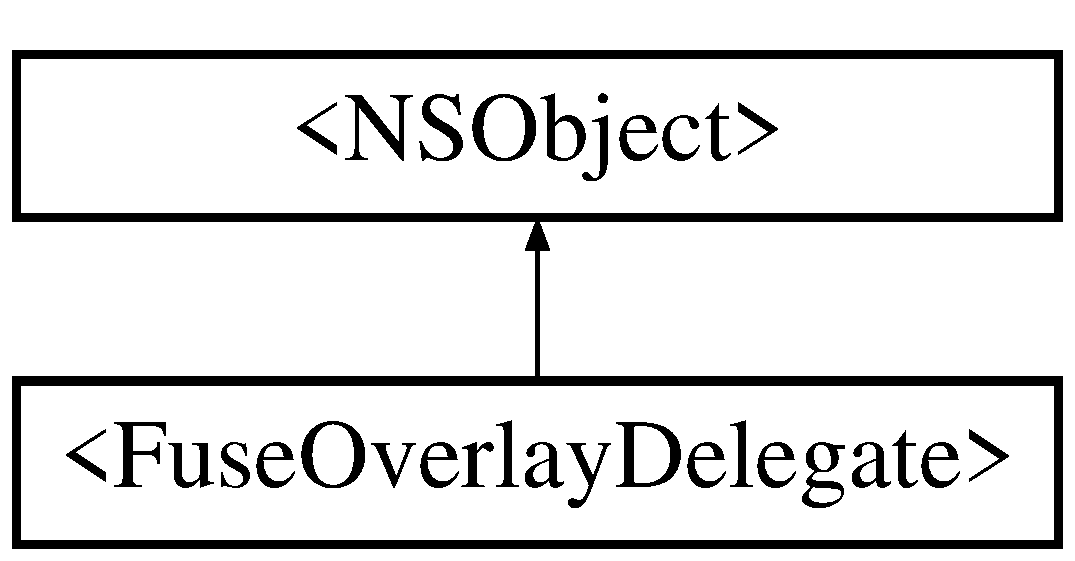
\includegraphics[height=2.000000cm]{protocol_fuse_overlay_delegate-p}
\end{center}
\end{figure}
\subsection*{Instance Methods}
\begin{DoxyCompactItemize}
\item 
(void) -\/ \hyperlink{protocol_fuse_overlay_delegate-p_a45f598193363390e2d50f9cec694be35}{overlay\+Will\+Close}
\begin{DoxyCompactList}\small\item\em This method indicates when a Fuse overlay will close. \end{DoxyCompactList}\end{DoxyCompactItemize}


\subsection{Detailed Description}
This is Fuse A\+P\+I overlay delegate. 

This delegate handles any event from a fuse overlay. Most commonly, an overlay will occur in the form of the \char`\"{}\+More Games\char`\"{} section. 

\subsection{Method Documentation}
\hypertarget{protocol_fuse_overlay_delegate-p_a45f598193363390e2d50f9cec694be35}{}\index{Fuse\+Overlay\+Delegate-\/p@{Fuse\+Overlay\+Delegate-\/p}!overlay\+Will\+Close@{overlay\+Will\+Close}}
\index{overlay\+Will\+Close@{overlay\+Will\+Close}!Fuse\+Overlay\+Delegate-\/p@{Fuse\+Overlay\+Delegate-\/p}}
\subsubsection[{overlay\+Will\+Close}]{\setlength{\rightskip}{0pt plus 5cm}-\/ (void) overlay\+Will\+Close 
\begin{DoxyParamCaption}
{}
\end{DoxyParamCaption}
\hspace{0.3cm}{\ttfamily [optional]}}\label{protocol_fuse_overlay_delegate-p_a45f598193363390e2d50f9cec694be35}


This method indicates when a Fuse overlay will close. 

When an overlay is being displayed by the application, most commonly the \char`\"{}\+More Games\char`\"{} overlay, and has been dismissed by the user, this method will be called to indicate that the application can continue execution of the user flow or application (if applicable). Often, the \char`\"{}\+More Games\char`\"{} section will be displayed over a menu, so the when the overlay is dismissed the menu will still be showing, thus not requiring the implementation of this method. \begin{DoxySeeAlso}{See also}
\hyperlink{interface_fuse_a_p_i_aced6aa0cc51278b431c664c3f5f9fc30}{+ display\+More\+Games\+: (\+Fuse\+A\+P\+I)} for more information on calling the More Games overlay 
\end{DoxySeeAlso}


The documentation for this protocol was generated from the following file\+:\begin{DoxyCompactItemize}
\item 
/\+Users/buildmachine/buildmonkey/\+Fuse\+S\+D\+Ki\+O\+S-\/master/\+Code/\+Classes/\+Fuse\+A\+P\+I/Fuse\+A\+P\+I.\+h\end{DoxyCompactItemize}

%--- End generated contents ---

% Index
\backmatter
\newpage
\phantomsection
\clearemptydoublepage
\addcontentsline{toc}{chapter}{Index}
\printindex

\end{document}
